\ifx\wholebook\relax \else
\documentclass[b5paper]{ctexart}
\usepackage[nomarginpar
  %, margin=.5in
]{geometry}

\addtolength{\oddsidemargin}{-0.05in}
\addtolength{\evensidemargin}{-0.05in}
\addtolength{\textwidth}{0.1in}
\usepackage[cn]{../prelude}

\setcounter{page}{1}

\begin{document}

\title{搜索}

\author{刘新宇
\thanks{{\bfseries 刘新宇 } \newline
  Email: liuxinyu95@gmail.com \newline}
  }

\maketitle
\fi

\markboth{搜索}{基本算法}

\ifx\wholebook\relax
\chapter{搜索}
\numberwithin{Exercise}{chapter}
\fi

\def\includetikz{}

现代计算机系统使很多困难的搜索问题得以实现。工业机器人可以从堆在生产线旁的零件中找出正确的进行组装,带有卫星导航系统的汽车可以在地图中找到前往目的地的最佳路线,智能手机还能搜索出最便宜的购物方案。本章介绍最基本的查找、匹配、图搜索算法。

\section{$k$选择问题}
\index{$k$选择}

这一问题是说如何在$n$个元素中寻找第$k$大(或小)的元素。这里大小的含义是抽象的序关系。我们先用$\leq$关系找出第$k$小的元素,然后再推广到其它一般情况。最简单的方法是先找到最小的,然后在剩余元素中寻找第二小的。进行$k$次就可以找到第$k$小的元素。在$n$个元素中寻找最小元素是线性时间$O(n)$的。因此总时间为$O(kn)$。我们也可以利用堆。这样可以在$O(\lg n)$时间内更新、获取顶部,重复$k$次可以在$O(k \lg n)$时间内获得答案。

\be
top\ k\ xs = find\ k\ (\textit{heapify}\ xs)
\ee

或写成柯里化形式:

\be
top\ k\ = (find\ k) \circ \textit{heapify}
\label{eq:kth-heap1}
\ee

其中:

\be
\begin{array}{rcl}
find\ 0 & = & top \\
find\ k & = & (find\ (k - 1)) \circ pop
\end{array}
\label{eq:kth-heap2}
\ee

我们还能找到更好的方法。使用分治策略将元素划分为$A$、$B$,使得$A$中元素都不大于($\leq$)$B$中元素。令$m = |A|$为$A$的大小,比较$m$和$k$:

\begin{enumerate}
\item 若$k < m$,则第$k$小的元素在$A$中,我们丢弃$B$,然后在$A$中递归查找;
\item 若$m < k$,则第$k$小的元素在$B$中,我们丢弃$A$,然后在$B$中递归查找第$(k-m)$小的元素。
\end{enumerate}

理想情况下划分是平衡的,$A$、$B$大小相当,每次问题规模减半,复杂度为$O(n + n/2 + n/4 +...) = O(n)$。我们利用上一章快速排序中的划分方法\textit{part},随机选择一个元素(如第一个)作为基准$p$。将所有$\leq p$的元素放入$A$,剩余元素放入$B$。这样若$m = k - 1$,则$p$就是第$k$小的元素,否则我们递归在$A$或$B$中查找。

\be
top\ k\ (x \cons xs) = \begin{cases}
  m = k - 1: & x, \text{其中}: m = |A|, (A, B) = part\ (\leq x)\ xs \\
  m < k - 1: & top\ (k - m - 1)\ B \\
  \text{否则}: & top\ k\ A \\
\end{cases}
\ee

和快速排序一样,最差情况下划分结果总不平衡,性能退化为$O(kn)$或$O((n-k)n)$。平均情况下可以在线性时间内找到答案。我们也可以应用快速排序划分中各种改进,如三点中值法\footnote{Blum、Floyd、Pratt、Rivest和Tarjan在1973年给出了一个线性时间方法\cite{CLRS}\cite{median-of-median}。将列表划分为若干组,每组最多5个元素,总共选出$n/5$个中值。重复这一步骤选出中值的中值。}和随机划分法:

\begin{algorithmic}[1]
\Function{Top}{$k, A, l, u$}
  \State \textproc{Exchange} $A[l] \leftrightarrow A[$ \Call{Random}{$l, u$} $]$ \Comment{随机在$[l, u]$内选择}
  \State $p \gets$ \Call{Partition}{$A, l, u$}
  \If{$p - l + 1 = k$}
    \State \Return $A[p]$
  \EndIf
  \If{$k < p - l + 1$}
    \State \Return \Call{Top}{$k, A, l, p-1$}
  \EndIf
  \State \Return \Call{Top}{$k - p + l - 1, A, p + 1, u$}
\EndFunction
\end{algorithmic}

我们可以调整这一方法获取全部的前$k$个值($k$个值间的顺序是任意的),如下面的例子程序:

\lstset{frame = single}
\begin{Haskell}
tops _ [] = []
tops 0 _  = []
tops n (x:xs) | len == n = as
              | len <  n = as ++ [x] ++ tops (n - len - 1) bs
              | otherwise = tops n as
    where
      (as, bs) = partition (<= x) xs
      len = length as
\end{Haskell}

\section{二分查找}
\index{二分查找}

中学时候老师表演过一个“数学魔术”:学生随便想一个1000以内的数,老师问十个问题,学生回答是或否。然后老师就能猜出这个数。例如:是偶数么?是素数么?所有位上的数字都相同么?能被3整除么?等等。神奇的是,老师总能猜到答案。在1000以内,如果每次通过问答排除一半数字,10次内就能找出答案。因为$2^{10} = 1024 > 1000$。“是偶数么?”就是一个非常好的问题,它能去掉一半的数字\footnote{社交网络上曾有一个“读心术”游戏。玩家暗想世界上任何一个人,人工智能机器人提16个问题,玩家回答是或否,最后机器人能说出玩家暗想的人是谁。}。设计奇偶性这样的问题需要一定的技巧,但存在着简单的方法每次淘汰掉一半。我们经常在电视里看到这样的竞猜节目。主持人展示一件商品,然后让观众猜价格。并告之是猜高了还是低了。如果能够在30秒内猜对,就获得奖励。例如:1000元,高了;500元,低了;750元,低了;890元,低了;990元,正确!这位观众使用了“二分查找”策略。为了在已序序列$A$中寻找$x$,我们找到位于序列中点上的$y$,和$x$比较。如果$x = y$,查找结束;如果$x < y$,由于$A$是已序的,我们只需要在前半部分继续查找;否则在后半部分查找。这样不断缩小$A$的规模,如果当$A = [\ ]$时仍未找到,则$x$不存在。二分查找要求$A$是已序的,我曾经看到有人试图对未排序的数组二分查找,深陷其中却得不到答案。高德纳说:“虽然二分查找的基本思想相对直观,具体细节却复杂得不可思议……”。本特利发现大多数二分查找的实现中含有错误。有趣的是他本人在《编程珠玑》第一版中给出的实现也包含了一个错误,直到20多年后才被发现\cite{Bentley}。下面给出了二分查找的实现,令数组$A$的上下界为$l$、$u$(不含$u$)。

\be
\textit{bsearch}\ x\ A\ (l, u) = \begin{cases}
  u < l: & \textit{Nothing} \\
  x = A[m]: & m, \text{其中}: m =  l + \lfloor \dfrac{u - l}{2} \rfloor \\
  x < A[m]: & \textit{bsearch}\ x\ A\ (l, m - 1) \\
  \text{否则}: & \textit{bsearch}\ x\ A\ (m + 1, u) \\
\end{cases}
\ee

我们也可以消除递归,通过更新边界实现二分查找:

\begin{algorithmic}[1]
\Function{Binary-Search}{$x, A, l, u$}
  \While{$l < u$}
    \State $m \gets l + \lfloor \dfrac{u - l}{2} \rfloor$ \Comment{避免$\lfloor \dfrac{l+u}{2} \rfloor$溢出}
    \If{$A[m] = x$}
      \State \Return $m$
    \EndIf
    \If{$x < A[m]$}
      \State $u \gets m - 1$
    \Else
      \State $l \gets m + 1$
    \EndIf
  \EndWhile
  \State Not found
\EndFunction
\end{algorithmic}

由于每次将数组减半,二分查找的复杂度为$O(\lg n)$。二分查找还可以搜索单调函数的解。例如方程$a^x = y$,其中$a \leq y$,$a$、$y$都是自然数,我们寻找$x$的整数解。我们可以穷举:从0开始依次尝试$a^0, a^1, a^2, ...$,直到发现某个$a^i = y$,或者$a^i < y < a^{i+1}$,表示方程无整数解。对很大的$a$和$x$,如果需要保持精度,则计算$a^x$会消耗一定的时间\footnote{当然,我们可以复用$a^n$的结果来计算$a^{n+1} = a a^n$。这里我们考虑一般意义下的单调函数$f(n)$。}。我们可以用二分查找来进行改进。首先估计解的上限。由于$a^y \geq y$,我们可以在区间$[0, 1, ..., y]$内搜索。由于函数$f(x) = a^x$是非减函数,对于自变量$x$,我们先检查区间中点$x_m = \lfloor \dfrac{0 + y}{2} \rfloor$,如果$a^{x_m} = y$,则$x_m$是方程的解;如果$a^{m} < y$,我们丢弃$x_m$前的部分;否则丢弃$x_m$后的部分;两种情况下都将搜索范围减半,直到找到解或查找范围变成空,表示无整数解。下面是二分查找解的定义。我们将单调函数抽象为一个参数$f$,调用$bsearch\ f\ y\ (0, y)$,其中$f(x) = a^x$。我们只需要计算$O(\lg y)$次$f(x)$,好于穷举法。

\be
\textit{bsearch}\ f\ y\ (l, u) = \begin{cases}
  u < l: & \textit{Nothing}  \\
  f(m) = y: & m, \text{其中}: m = \lfloor \dfrac{l + u}{2} \rfloor \\
  f(m) < y: & \textit{bsearch}\ f\ y\ (m + 1, u) \\
  f(m) > y: & \textit{bsearch}\ f\ y\ (l, m - 1) \\
  \end{cases}
\label{eq:bsearch}
\ee

\subsection{二维查找}

考虑把二分查找从一维扩展到二维或更高维。令矩阵$M$的大小为$m \times n$。每行、每列的元素都是单调增加的自然数。如\cref{fig:matrix-eg}所示。如何快速地在矩阵中找到所有等于$z$的元素呢?我们需要给出一个算法,返回一组位置$(i, j)$的列表,使得所有的$M_{i,j} = z$

\be
[(x, y) | x \gets [1, 2,..., m], y \gets [1, 2,..., n], M_{x, y} = z]
\label{eq:bsearch-brute}
\ee

\begin{figure}[htbp]
 \centering
\[
\left [
  \begin{array}{ccccc}
    1 & 2 & 3 & 4 & ... \\
    2 & 4 & 5 & 6 & ... \\
    3 & 5 & 7 & 8 & ... \\
    4 & 6 & 8 & 9 & ... \\
    ... \\
  \end{array}
\right ]
\]
\caption{每行、每列都单调增加}
\label{fig:matrix-eg}
\end{figure}

理查德$\cdot$伯德曾用这一问题面试学生\cite{fp-pearls}。那些在中学就接触编程的学生往往尝试二分查找来解题,但却很容易陷入困境。按照二分查找的思路,通常先检查位于$M_{\frac{m}{2}, \frac{n}{2}}$上的元素。如果它小于$z$,我们丢弃左上区域;如果大于$z$,丢弃右下区域,如\cref{fig:bsearch-2D}所示,灰色的区域表示可丢弃。两种情况下,搜索区域都从一个矩形变成了一个L形,无法直接递归。我们把这类二维搜索问题抽象为:已知函数$f(x, y)$,在某一范围内寻找整数解$(x, y)$,使得$f(x, y) = z$。矩阵搜索可以特化为下面的函数:

\begin{figure}[htbp]
 \centering
 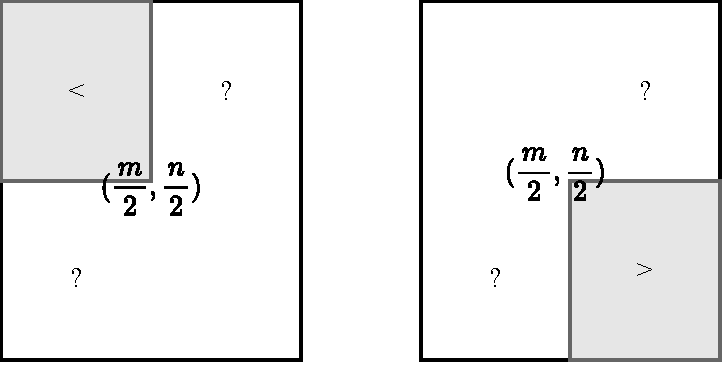
\includegraphics[scale=0.5]{img/binary-search-2d}
 \caption{左:中点元素小于$z$,灰色区域都小于$z$;右:中点元素大于$z$。灰色区域都大于$z$。}
 \label{fig:bsearch-2D}
\end{figure}

\[
f(x, y) = \begin{cases}
  1 \leq x \leq m, 1 \leq y \leq n: & M_{x, y} \\
  \text{其它}: & -1 \\
  \end{cases}
\]

\index{马鞍搜索}
如果$f(x, y)$是单调增函数,例如$f(x, y) = x^a + y^b$,$a$、$b$是自然数,有效解法不是从左下角出发,而是从左上角出发开始查找\cite{saddle-back}。如\cref{fig:saddleback-1}所示,搜索从$(0, z)$开始,对于每个点$(p, q)$,我们比较$f(p, q)$和$z$的关系:

\begin{enumerate}
\item 如果$f(p, q) < z$:由于$f$单调增,所有的$0 \leq y < q$,有$f(p, y) < z$。我们丢弃垂直线段上的所有点(红色线段);
\item 如果$f(p, q) > z$:所有的$p < x \leq z$,有$f(x, q) > z$。我们丢弃水平线段上的所有点(蓝色线段);
\item 如果$f(p, q) = z$:$(p, q)$是一个解,两条线段上的点都可以丢弃。
\end{enumerate}

这样,我们就可以逐步缩小矩形搜索区域。每次要么丢弃一行,要么丢弃一列,或者同时丢弃行、列。

\begin{figure}[htbp]
 \centering
 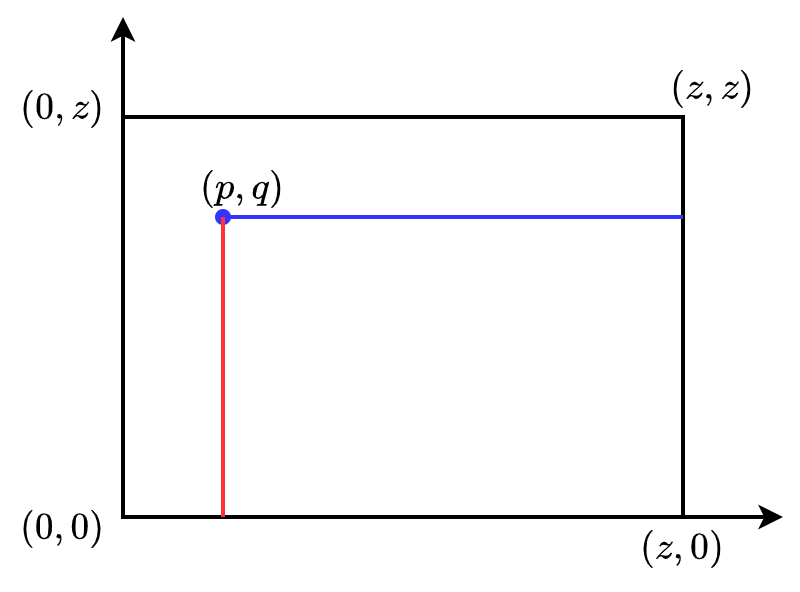
\includegraphics[scale=0.2]{img/saddle-back-start}
 \caption{从左上角搜索}
 \label{fig:saddleback-1}
\end{figure}

定义\textit{search}函数,并传入左上角开始搜索:$search(f, z, 0, z)$。

\be
\textit{search}\ f\ z\ p\ q\ =  \begin{cases}
  p > z \text{或} q < 0: & [\ ]   \\
  f(p, q) < z: & \textit{search}\ f\ z\ (p + 1)\ q  \\
  f(p, q) > z: & \textit{search}\ f\ z\ p\ (q - 1)  \\
  f(p, q) = z: & (p, q) : \textit{search}\ f\ z\ (p + 1)\ (q - 1) \\
  \end{cases}
\ee

每次查找后,$p$、$q$至少有一个会向右、下前进一步。最多需要$2(z+1)$次查找完成搜索。最好情况有三种:(1)每次$p$、$q$同时前进一步,只要$z+1$步就完成搜索;(2)不断水平向右前进,最后$p$超过$z$;(3)不断垂直向下前进,最终$q$变为负。\cref{fig:saddleback-1-cases}描述了最好和最坏的情况。\cref{fig:saddleback-1-cases} (a)中,对角线上的每个点$(x, z-x)$都满足$f(x, z-x) = z$,总共需要$z+1$步到达$(z, 0)$;(b)中,上方水平线的每个点$(x, z)$都使得$f(x, z) < z$,$z+1$步后,搜索结束;(c)中,左侧垂线的每个点$(0, x)$都使得$f(0, x) > z$,$z+1$步后,搜索结束;(d)描述的是最差情况。如果我们将搜索路径上的所有水平线段投射$x$轴上,所有垂直线段投射到$y$轴上,就可以得到总共的搜索步数为$2(z+1)$。和复杂度为$O(z^2)$的穷举法相比,这一改进将复杂度提高到线性时间$O(z)$。

\begin{figure}[htbp]
 \centering
 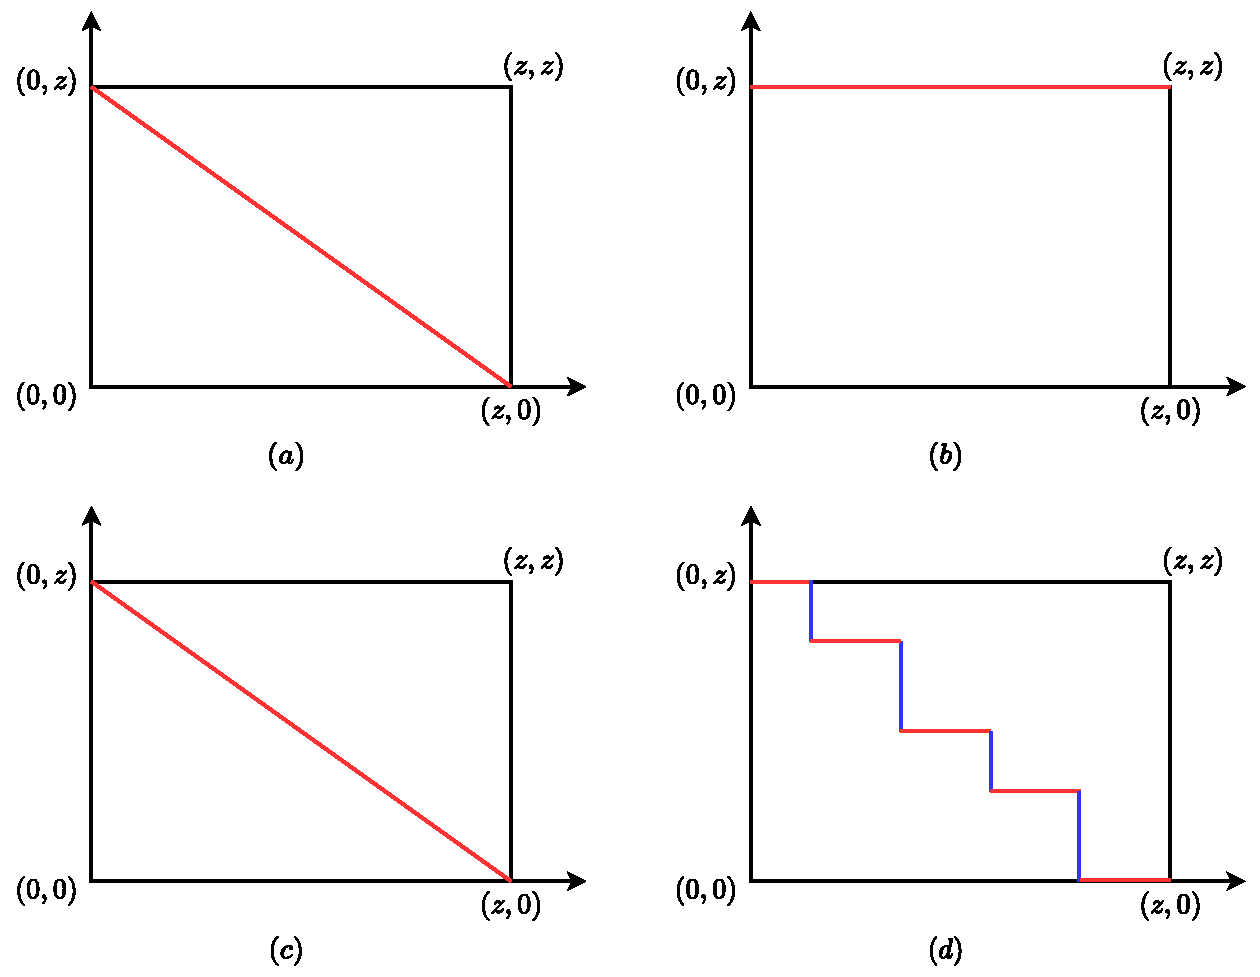
\includegraphics[scale=0.15]{img/saddle-back-paths}
 \caption{最好和最差情况}
 \label{fig:saddleback-1-cases}
\end{figure}

这一方法叫做“马鞍搜索”。函数$f$的三维图像中,左下部的最小值和右上部的最大值,以及两侧的翼形图像,合起来像一个马鞍。如\cref{fig:saddleback-frame}所示。马鞍搜索从左上角$(0, z)$向右下角$(z, 0)$搜索。这一范围可进一步缩小。$f$单调增,我们可以沿$y$轴找到最大$m$,使得$f(0, m) \leq z$;沿$x$轴找到最大$n$,使得$f(n, 0) \leq z$;这样搜索区域就从$(0, z) - (z, 0)$缩小到$(0, m) - (n, 0)$,如\cref{fig:saddleback-2}所示。

\begin{figure}[htbp]
 \centering
 \includegraphics[scale=0.8]{img/saddleback-xx-yy}
 \caption{$f(x, y) = x^2 + y^2$的图像}
 \label{fig:saddleback-frame}
\end{figure}

\begin{figure}[htbp]
 \centering
 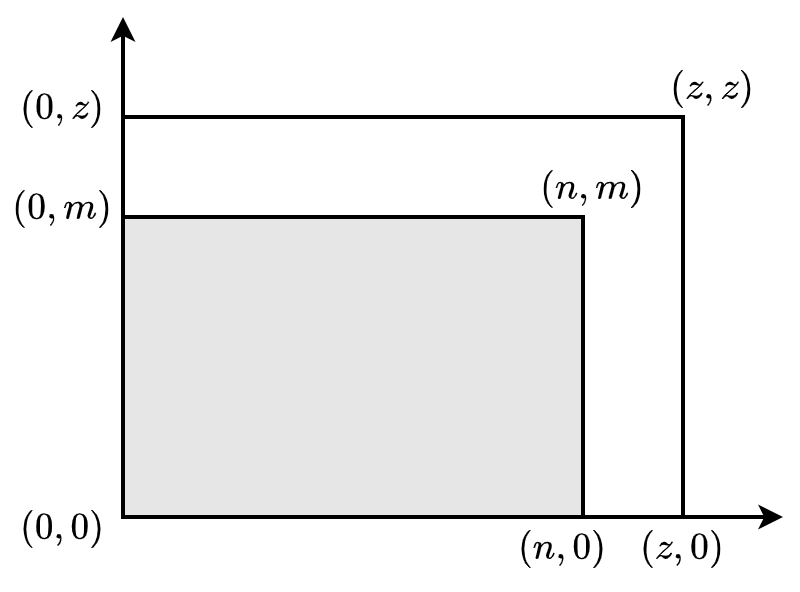
\includegraphics[scale=0.2]{img/saddle-back-area}
 \caption{缩小的灰色搜索区域}
 \label{fig:saddleback-2}
\end{figure}

\be
\begin{cases}
m & = \max\ [y | 0 \leq y \leq z, f(0, y) \leq z] \\
n & = \max\ [x | 0 \leq x \leq z, f(x, 0) \leq z]
\end{cases}
\ee

我们可以用二分查找搜索$m$、$n$(固定$x = 0$查找$m$,固定$y = 0$查找$n$)。改动\cref{eq:bsearch}的定义,给定$y$,寻找$l \leq x \leq u$满足$f(x) \leq y < f(x+1)$

\be
\textit{bsearch}\ f\ y\ (l, u) = \begin{cases}
  u \leq l: & l \\
  f(m) \leq y < f(m + 1): & m, \text{其中}: m = \lfloor \dfrac{l + u}{2} \rfloor \\
  f(m) \leq y: & \textit{bsearch}\ f\ y\ (m + 1, u) \\
  f(m) > y : & \textit{bsearch}\ f\ y\ (l, m - 1)  \\
  \end{cases}
\label{eq:bsearch-general}
\ee

这样就可以二分查找$m$、$n$:

\be
\begin{cases}
m & = \textit{bsearch}\ (y \mapsto f(0, y))\ z\ (0, z) \\
n & = \textit{bsearch}\ (x \mapsto f(x, 0))\ z\ (0, z) \\
\end{cases}
\label{eq:bsearch-boundaries}
\ee

接下来在缩小的矩形内进行马鞍搜索:$solve(f, z) = search(f, z, 0, \pmb{m})$

\be
\textit{search}\ f\ z\ p\ q\ =  \begin{cases}
  p > \pmb{n} \text{或} q < 0: & [\ ]   \\
  f(p, q) < z: & \textit{search}\ f\ z\ (p + 1)\ q  \\
  f(p, q) > z: & \textit{search}\ f\ z\ p\ (q - 1)  \\
  f(p, q) = z: & (p, q) : \textit{search}\ f\ z\ (p + 1)\ (q - 1) \\
  \end{cases}
\ee

这一改进首先用两轮二分查找得到$m$和$n$,每轮计算了$O(\lg z)$次$f$;马鞍搜索在最坏情况下计算$O(m+n)$次$f$;最好情况下计算$O(\min(m, n))$次。总体复杂度如下表。某些函数如$f(x, y) = x^a + y^b$,对于自然数$a$、$b$,边界$m$、$n$很小,整体性能接近$O(\lg z)$。

\btab{|l|l|}
\hline
 & 计算$f$的次数 \\
\hline
最坏情况 & $2 \log z + m + n$ \\
最好情况 & $2 \log z + \min(m, n)$ \\
\hline
\etab

如\cref{fig:saddleback-drop},考虑搜索区域$(a, b) - (c, d)$中的一点$(p, q)$,若$f(p, q) \neq z$,只能丢弃灰色部分($\leq 1/4$)。如果$f(p, q) = z$,由于$f$单调增,我们可同时丢弃左下、右上部分,和$p$列、$q$行上的其它点。这样只剩下1/2的区域,可以快速缩小搜索范围。为了找到$f(p, q) = z$的点,我们沿着矩形中心水平线或中心垂直线应用二分查找。在线段$L$上二分查找的复杂度为$O(\lg |L|)$,我们选取较短的中线搜索,如\cref{fig:saddleback-centerline}所示。

\begin{figure}[htbp]
 \centering
 \subcaptionbox{如果$f(p, q) \neq z$,只能丢弃左下或右上的灰色区域,剩余区域变成了L形。}{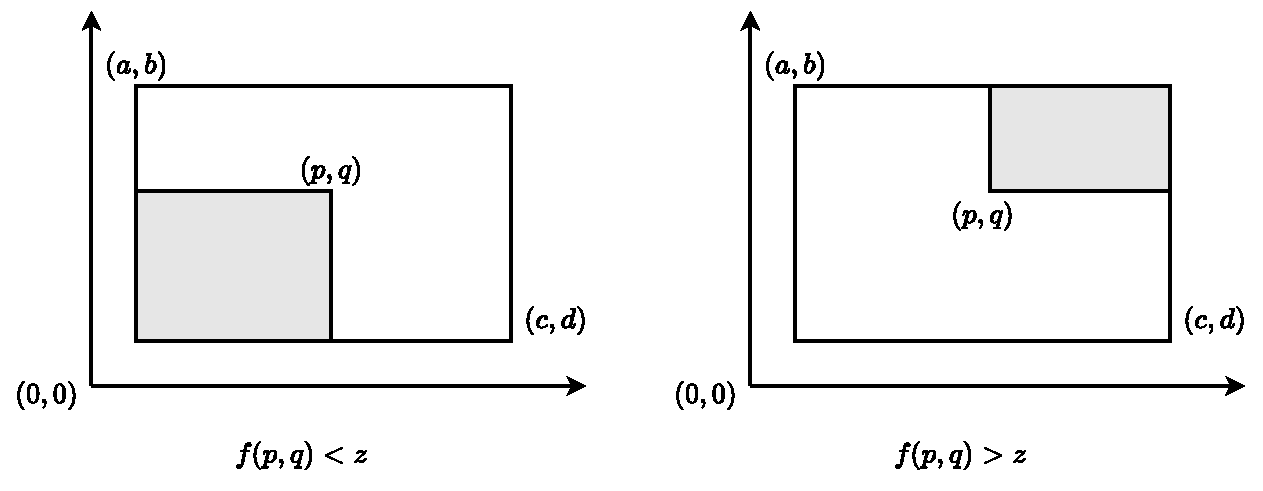
\includegraphics[scale=0.2]{img/saddleback-l-area}} \\
 \subcaptionbox{如果$f(p, q) = z$,可同时丢弃两个灰色部分,搜索区域减半。}{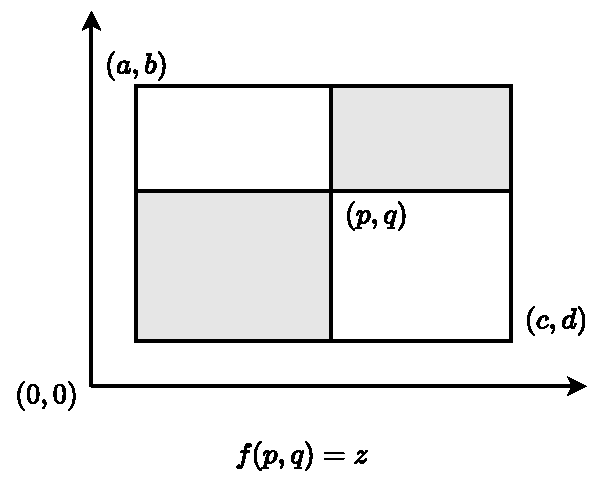
\includegraphics[scale=0.2]{img/saddleback-half-area}}
 \caption{缩小搜索区域}
 \label{fig:saddleback-drop}
\end{figure}

\begin{figure}[htbp]
 \centering
 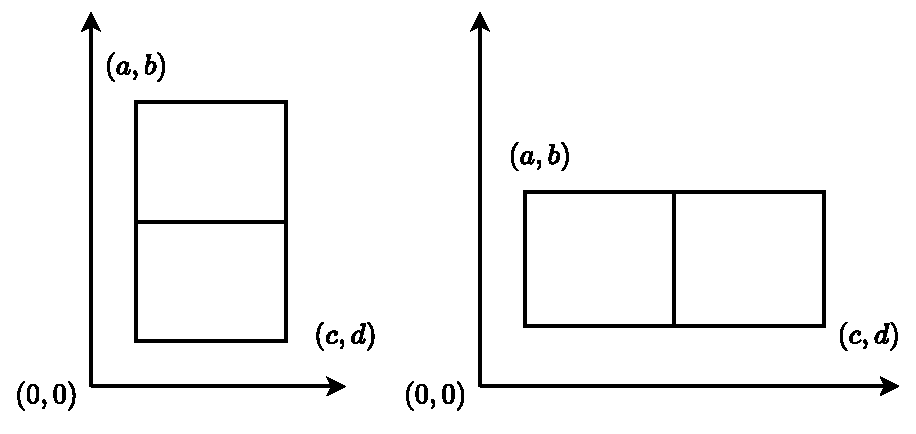
\includegraphics[scale=0.2]{img/saddleback-mid-line}
 \caption{沿较短的中线二分查找}
 \label{fig:saddleback-centerline}
\end{figure}

如果中线上不存$f(p, q) = z$的点,我们寻找满足$f(p, q) < z < f(p + 1, q)$的点(水平中线,对于垂直中线为$f(p, q) < z < f(p, q + 1)$)。此时我们不能将$p$列、$q$行上的点完全丢弃。综合起来,我们用二分查找搜索水平中线上满足$f(p, q) \leq z < f(p + 1, q)$的点,或中垂直线上满足$f(p, q) \leq z < f(p, q + 1)$的点。如果线段上所有点都使得$f(p, q) < z$,则返回上界;如果所有点都使得$f(p, q) > z$,则返回下界。此时,我们丢弃中线一侧的区域。下面是改进的马鞍搜索:

\begin{enumerate}
\item 沿$x$、$y$轴二分搜索,确定搜索区域$(0, m) - (n, 0)$;
\item 若搜索区域$(a, b) - (c, d)$高大于宽,沿水平中线二分查找;否则沿中垂线二分查找,结果为点$(p, q)$;
\item 若$f(p, q) = z$,$(p, q)$为一个解。递归搜索子区域$(a, b) - (p-1, q+1)$和$(p+1, q-1) - (c, d)$;
\item 若$f(p, q) \neq z$,递归搜索两个子区域外和一条线段。线段为$(p, q+1) - (p, b)$,如\cref{fig:include-line} (a);或$(p+1, q) - (c, q)$,如\cref{fig:include-line} (b)。
\end{enumerate}

\begin{figure}[htbp]
 \centering
 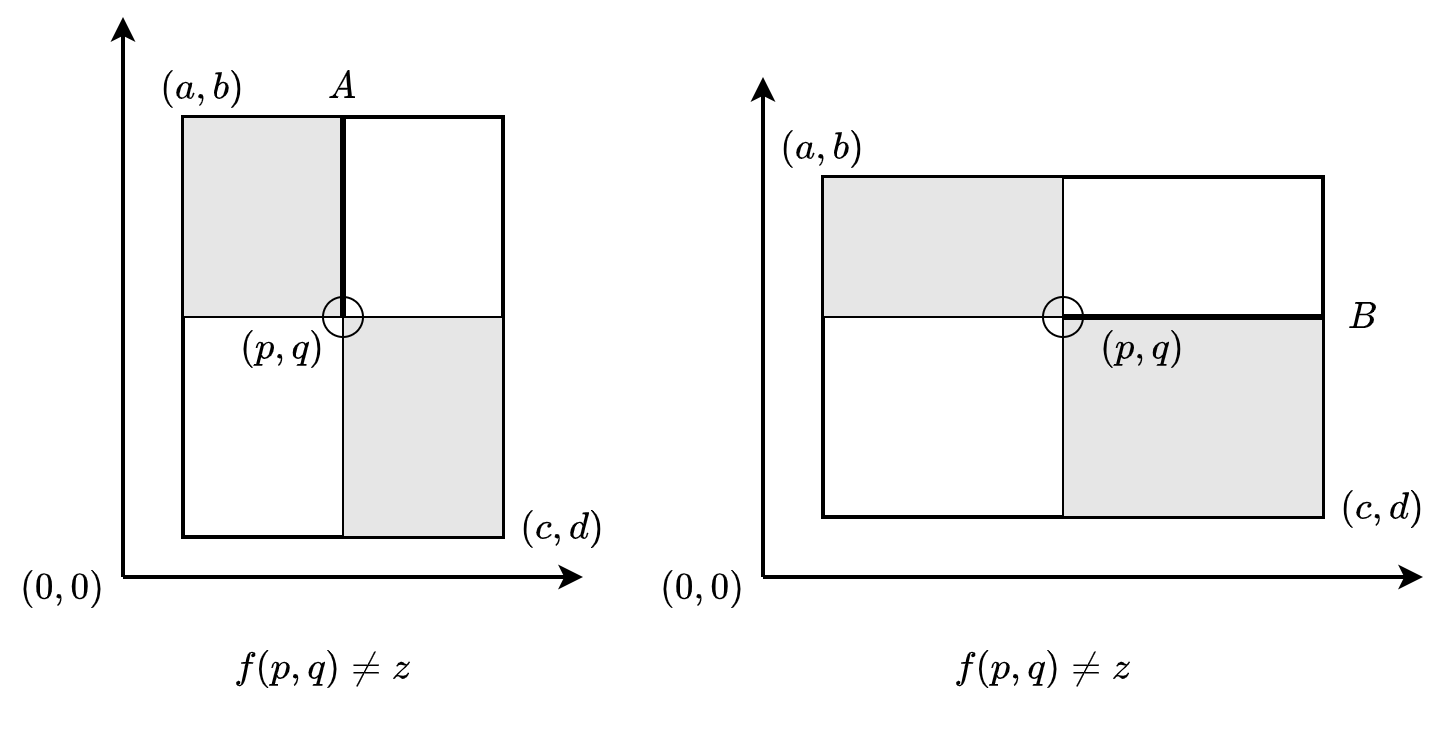
\includegraphics[scale=0.2]{img/saddleback-mid-line-inc}
 \caption{递归搜索灰色的区域,如果$f(p, q) \neq z$,还需要搜索加粗的线段。}
 \label{fig:include-line}
\end{figure}

\be
\textit{search}\ (a, b)\ (c, d) = \begin{cases}
  c < a \text{或} d < b: & [\ ] \\
  c - a < b - d: & \textit{csearch}  \\
  \text{否则}: & \textit{rsearch} \\
  \end{cases}
\ee

其中\textit{csearch}在水平中线上二分查找$(p, q)$使得$f(p, q) \leq z < f(p+1, q)$,如\cref{fig:include-line} (a)所示。如果中线上所有函数值大于$z$,返回下界$(a, \lfloor \dfrac{b + d}{2} \rfloor)$。丢弃中线上侧(含中线),如\cref{fig:saddleback-edge-cases} (a)所示。

\begin{figure}[htbp]
 \centering
 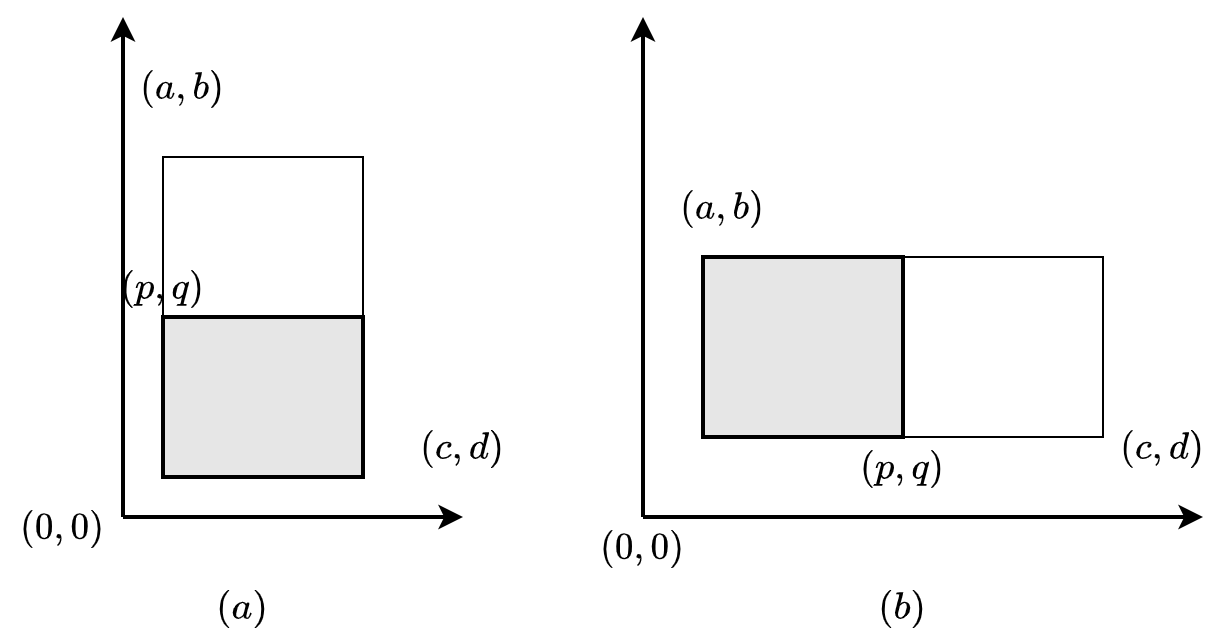
\includegraphics[scale=0.2]{img/saddleback-halve}
 \caption{沿中线二分查找时的特殊情况}
 \label{fig:saddleback-edge-cases}
\end{figure}

令:

\[
\begin{cases}
q = \lfloor \dfrac{b + d}{2} \rfloor \\
p = \textit{bsearch}\ (x \mapsto f(x, q))\ z\ (a, c) \\
\end{cases}
\]

\be
\resizebox{\textwidth}{!}{\ensuremath{
\textit{csearch} = \begin{cases}
  f(p, q) > z: & \textit{search}\ (p, q - 1)\ (c, d)  \\
  f(p, q) = z: & \textit{search}\ (a, b)\ (p - 1, q + 1) \doubleplus [(p, q)] \doubleplus \textit{search}\ (p + 1, q - 1)\ (c, d) \\
  f(p, q) < z: & \textit{search}\ (a, b)\ (p, q + 1) \doubleplus \textit{search}\ (p + 1, q - 1)\ (c, d) \\
  \end{cases}
}}
\ee

$rsearch$与此类似,沿中垂线搜索。下面的例子程序实现了改进的马鞍搜索:

\begin{Haskell}
solve f z = search f z (0, m) (n, 0) where
  m = bsearch (f 0) z (0, z)
  n = bsearch (\x -> f x 0) z (0, z)

search f z (a, b) (c, d)
       | c < a || b < d = []
       | c - a < b - d = let q = (b + d) `div` 2 in
           csearch (bsearch (\x -> f x q) z (a, c), q)
       | otherwise = let p = (a + c) `div` 2 in
           rsearch (p, bsearch (f p) z (d, b))
  where
    csearch (p, q)
        | z < f p q = search f z (p, q - 1) (c, d)
        | f p q == z = search f z (a, b) (p - 1, q + 1) ++
                 (p, q) : search f z (p + 1, q - 1) (c, d)
        | otherwise = search f z (a, b) (p, q + 1) ++
                 search f z (p + 1, q - 1) (c, d)
    rsearch (p, q)
        | z < f p q = search f z (a, b) (p - 1, q)
        | f p q == z = search f z (a, b) (p - 1, q + 1) ++
                 (p, q) : search f z (p + 1, q - 1) (c, d)
        | otherwise = search f z (a, b) (p - 1, q + 1) ++
                 search f z (p + 1, q) (c, d)
\end{Haskell}

搜索区域每次减半,总共搜索$O(\lg (mn))$轮。沿中线二分查找$(p, q)$,需要计算$f$共$O(\lg (\min(m, n)))$次。令在$m \times n$区域搜索时间为$T(m, n)$,有如下的递归关系:

\be
T(m, n) = \lg(\min(m, n)) + 2 T(\dfrac{m}{2}, \dfrac{n}{2})
\ee

不妨设$m = 2^i > n = 2^j$,使用裂项求和法:

\be
\begin{array}{rl}
T(2^i, 2^j) & = j + 2 T(2^{i-1}, 2^{j-1}) \\
            & = \displaystyle \sum_{k=0}^{i-1} 2^k(j - k) \\
            & = O(2^i(j-i)) \\
            & = O(m \lg (n/m))
\end{array}
\ee

伯德证明了这是在$m \times n$区域内搜索的最优下界\cite{fp-pearls}。

\begin{Exercise}\label{ex:binary-search}
\Question{证明$k$选择的平均复杂度为$O(n)$。}
\Question{为了查找$A$中的前$k$小元素,我们可以获取$x = \max\ (take\ k\ A), y = \min\ (drop\ k\ A)$。如果$x < y$,则$A$的前$k$个元素就是答案;否则我们用$x$划分前$k$个元素,用$y$划分剩余元素,然后在子序列$[a | a \gets A, x < a < y]$中递归查找前$k'$个元素,其中$k' = k - |[a | a \gets A, a \leq x]|$。请实现这一算法,并分析复杂度。
}
\Question{查找两个已序数组$A$和$B$的“简化中值”,满足时间复杂度$O(\lg (m + n))$,其中$m = |A|, n = |B|$,分别为两个数组的长度。数组下标从0开始。简化中值定义为: $median(A, B) = C[\lfloor \dfrac{m + n}{2} \rfloor]$,其中$C = merge(A, B)$为合并后的已序数组\footnote{简化定义与常见的统计学定义不同。后者对于含有$n$个元素升序序列$x$的中值定义为:
\[
median(x) = \begin{cases}
odd(n): & x[\frac{n + 1}{2}] \\
even(n): & \dfrac{1}{2}(x[\dfrac{n}{2}] + x[\dfrac{n}{2}+1]) \\
\end{cases}
\]
}
。}
\Question{消除递归,通过更新搜索边界实现马鞍查找。}
\Question{实现二维搜索算法并分析复杂度:矩形搜索区域的左下角是最小值,右上角是最大值。若搜索值$z$小于最小值或者大于最大值无解;否则从中心划一个十字,分割成4个小矩形,然后递归搜索。}
\end{Exercise}

\begin{Answer}[ref = {ex:binary-search}]
\Question{证明$k$选择的平均复杂度为$O(n)$。

参考快速排序的复杂度分析\cref{sec:quick-sort-big-o}。}

\Question{为了查找$A$中的前$k$小元素,我们可以获取$x = \max\ (take\ k\ A), y = \min\ (drop\ k\ A)$。如果$x < y$,则$A$的前$k$个元素就是答案;否则我们用$x$划分前$k$个元素,用$y$划分剩余元素,然后在子序列$[a | a \gets A, x < a < y]$中递归查找前$k'$个元素,其中$k' = k - |[a | a \gets A, a \leq x]|$。请实现这一算法,并分析复杂度。

\begin{algorithmic}[1]
\Procedure{Tops}{$k, A$}
  \State $l \gets 1$
  \State $u \gets |A|$
  \Loop
    \State $i \gets$ \Call{Max-At}{$A[l..k]$}
    \State $j \gets$ \Call{Min-At}{$A[k+1..u]$}
    \If{$A[i] < A[j]$}
      \State break
    \EndIf
    \State \textproc{Exchange} $A[l] \leftrightarrow A[j]$
    \State \textproc{Exchange} $A[k+1] \leftrightarrow A[i]$
    \State $l \gets$ \Call{Partition}{$A, l, k$}
    \State $u \gets$ \Call{Partition}{$A, k+1, u$}
  \EndLoop
\EndProcedure
\end{algorithmic}

平均情况下的复杂度是$O(n)$。分析思路大致为:每轮循环用线性时间找到最大、最小值$i, j$,然后执行两轮线性时间的划分。如果划分平衡,分摊下来每次平均丢弃一半元素。这样总时间为$O(n + n/2 + n/4...) = O(n)$。
}

\Question{查找两个已序数组$A$和$B$的“简化中值”,满足时间复杂度$O(\lg (m + n))$,其中$m = |A|, n = |B|$,分别为两个数组的长度。数组下标从0开始。简化中值定义为: $median(A, B) = C[\lfloor \dfrac{m + n}{2} \rfloor]$,其中$C = merge(A, B)$为合并后的已序数组\footnote{简化定义与常见的统计学定义不同。后者对于含有$n$个元素升序序列$x$的中值定义为:
\[
median(x) = \begin{cases}
odd(n): & x[\frac{n + 1}{2}] \\
even(n): & \dfrac{1}{2}(x[\dfrac{n}{2}] + x[\dfrac{n}{2}+1]) \\
\end{cases}
\]
}。

我们给出两个方法。第一个方法在两个数组中分别进行二分查找。令$l = 0$、$u = m$,我们猜测中值在$A$中的索引为:$i = \lfloor \frac{l + u}{2} \rfloor$。根据简化中值的定义,共有$h = \lfloor \frac{m + n}{2} \rfloor$个元素在它之前。其中,$A$中有$i$个元素在$A[i]$之前,如果猜测正确,则在$B$中应有$j = h - i$个元素在$A[i]$之前。检查不等式$B[j] \leq A[i] \leq B[j + 1]$。如果成立,说明猜测的$A[i]$就是中值。否则根据偏大或偏小调整$l$、$u$重新二分查找。下面的例子程序实现了这一方法:

\begin{Bourbaki}
K median([K] a, [K] b) {
    if a == [] then return b[length(b) / 2]
    if b == [] then return a[length(a) / 2]
    Int i = medianOf(a, b)
    return if i == -1 then return median(b, a) else a[i]
}

Int medianOf([K] a, [K] b) {
    Int l = 0, u = length(a)
    while l < u {
        var i = (l + u) / 2
        var j = (length(a) + length(b)) / 2  - i
        if j < 1 or j >= len(b) {
            if (j == 0 and a[i] <= b[0]) or
               (j == len(b) and b[j - 1] <= a[i]) then return i
            if j >= len(b) then l = i + 1 else u = i
        } else {
            if b[j - 1]  <= a[i] and a[i] <= b[j] then return i
            if a[i] < b[j - 1] then l = i + 1 else u = i
        }
    }
    return -1
}
\end{Bourbaki}

第二种方法是利用一个通用的查找第$k$个元素的函数。假设$m \geq n$(否则交换$A$、$B$),如果任一数组为空,则返回另外一个的第$k$个元素。如果$k = 1$,返回$A[0]$、$B[0]$中较小的一个。否则猜测$j = min(k/2, n)$,$i = k - j$,然后比较$A[i]$和$B[j]$。如果$A[i] < B[j]$,我们丢弃所有$A[i]$前和$B[j]$后的元素,然后递归在剩余元素中寻找第$k-i$大的;否则丢弃所有$B[j]$前和$A[i]$后的,然后递归寻找第$k-j$大的元素。

\begin{Bourbaki}
K median([K] xs, [K] ys) {
    Int n = length(xs), m = length(ys)
    return kth(xs, 0, n, ys, 0, m, (m + n) / 2 + 1)
}

K kth([K] xs, Int x0, Int x1, [K] ys, Int y0, Int y1, Int k) {
    if x1 - x0 < y1 - y0 then return kth(ys, y0, y1, xs, x0, x1, k)
    if x1 <= x0 then return ys[y0 + k - 1]
    if y1 <= y0 then return xs[x0 + k - 1]
    if k == 1 then return min(xs[x0], ys[y0])
    var j = min(k / 2, y1 - y0), i = k - j
    i = x0 + i, j = y0 + j
    if xs[i - 1] < ys[j - 1] then
        return kth(xs, i, x1, ys, y0, j, k - i + x0)
    else
        return kth(xs, x0, i, ys, j, y1, k - j + y0)
}
\end{Bourbaki}

另外,我们不能这样定义简化中值:$m \in A \doubleplus B$,使得:
\[
|[y \gets A \doubleplus B, y < m]| - |[y \gets A \doubleplus B, y > m]| = 0, \pm 1
\]
考虑这样的反例:$[0, 1, 2, 3, 3, 3, 3, 3, 5]$,即使用小于等于、大于等于也会有问题。
}

\Question{消除递归,通过更新搜索边界实现马鞍查找。

\begin{algorithmic}[1]
\Function{Solve}{$f, z$}
  \State $p \gets 0, q \gets z$
  \State $S \gets \phi$
  \While{$p \leq z$ 且 $q \geq 0$}
    \State $z' \gets f(p, q)$
    \If{$z' < z$}
      \State $p \gets p + 1$
    \ElsIf{$z' > z$}
      \State $q \gets q - 1$
    \Else
      \State $S \gets S \cup \{(p, q)\}$
      \State $p \gets p + 1, q \gets q - 1$
    \EndIf
  \EndWhile
  \State \Return $S$
\EndFunction
\end{algorithmic}
}

\Question{实现二维搜索算法并分析复杂度:矩形搜索区域的左下角是最小值,右上角是最大值。若搜索值$z$小于最小值或者大于最大值无解;否则从中心划一个十字,分割成4个小矩形,然后递归搜索。

\begin{algorithmic}[1]
\Procedure{Search}{$f, z, a, b, c, d$} \Comment{$(a, b)$:左下角 $(c, d)$:右上角}
  \If {$z \leq f(a, b)$ 或 $f(c, d) \geq z$}
    \If{$z = f(a, b)$}
      \State record $(a, b)$ as a solution
    \EndIf
    \If{$z = f(c, d)$}
      \State record $(c, d)$ as a solution
    \EndIf
    \State \Return
  \EndIf
  \State $p \gets \lfloor \frac{a + c}{2} \rfloor$
  \State $q \gets \lfloor \frac{b + d}{2} \rfloor$
  \State \Call{Search}{$f, z, a, q, p, d$}
  \State \Call{Search}{$f, z, p, q, c, d$}
  \State \Call{Search}{$f, z, a, b, p, q$}
  \State \Call{Search}{$f, z, p, b, c, q$}
\EndProcedure
\end{algorithmic}

我们可以利用主定理进行递归复杂度分析:设在面积为$A$的矩形内搜索的时间为$T(A)$。我们用$O(1)$时间检查$z \leq f(a, b)$或$f(c, d) \geq z$是否成立,然后分割为4个小矩形递归:$T(A) = 4 T(A/4) + O(c)$。根据主定理复杂度为$O(A) = O(m n)$,和矩形的面积,即边长的乘积成正比。
}
\end{Answer}

\section{众数问题}
\index{Boyer-Moore众数问题}

人们常常投票并用计算机统计结果。某个小岛正在选举总统,只有赢得半数以上选票的候选人才可当选。从投票结果序列,如A, B, A, C, B, B, D, ...统计结果。能否高效找出当选总统?可以利用字典数据结构遍历选票来解决(见第2章)\footnote{2004年,人们发现了一种概率算法,称为Count-min sketch算法,使用sub-linear空间进行计数\cite{count-min-sketch}。}:

\begin{Bourbaki}
Optional<T> majority([T] xs) {
    Map<T, Int> m
    for var x in xs {
        if x in m then m[x]++ else mx[x] = 0
    }
    var (r, v) = (Optional<T>.Nothing, length(xs) / 2 - 1)
    for var (x, c) in m {
      if c > v then (r, v) = (Optional.of(x), c)
    }
    return r
}
\end{Bourbaki}

可以用红黑树或散列表实现的字典数据结构,如果有$m$名候选人$n$张选票,这一实现的复杂度如下表:

\btab{|l|l|l|}
\hline
字典 & 时间 & 空间 \\
\hline
红黑树 & $O(n \lg m)$ & $O(m)$ \\
\hline
散列表 & $O(n)$ & 最少$O(m)$ \\
\hline
\etab

超过一半的元素叫做“众数”。鲍耶和摩尔在1980年给出了一种方法,可以扫描一遍找出众数(如果存在)。算法的时间复杂度为$O(n)$,空间复杂度为$O(1)$,被称做鲍耶——摩尔众数算法\cite{boyer-moore-majority}。它建立在这样的想法上:众数最多只有1个,我们不断删掉两个不同的元素,直到最后剩下的元素都相等。如果众数存在,最后剩下的一定是众数。设第一张选票上的候选人为目前的获胜者,赢得的票数为1。依次检查后继选票,若选票还投给目前的获胜者,则获胜者的得票加1,否则获胜者得票减1。若得票减到0则不再是获胜者了。选择下一张选票上的候选人为新获胜者并继续,如下表所示。若存在众数$m$,则$m$不可能被其它元素超过落选。但如果众数不存在(选举无效,未决出优胜),则最后记录的“获胜者”并无意义。需要再扫描一轮进行验证。

\btab{|l|l|l|}
\hline
获胜者 & 得票 & 扫描位置 \\
\hline
A & 1 & \textbf{A}, B, C, B, B, C, A, B, A, B, B, D, B \\
A & 0 & A, \textbf{B}, C, B, B, C, A, B, A, B, B, D, B \\
C & 1 & A, B, \textbf{C}, B, B, C, A, B, A, B, B, D, B \\
C & 0 & A, B, C, \textbf{B}, B, C, A, B, A, B, B, D, B \\
B & 1 & A, B, C, B, \textbf{B}, C, A, B, A, B, B, D, B \\
B & 0 & A, B, C, B, B, \textbf{C}, A, B, A, B, B, D, B \\
A & 1 & A, B, C, B, B, C, \textbf{A}, B, A, B, B, D, B \\
A & 0 & A, B, C, B, B, C, A, \textbf{B}, A, B, B, D, B \\
A & 1 & A, B, C, B, B, C, A, B, \textbf{A}, B, B, D, B \\
A & 0 & A, B, C, B, B, C, A, B, A, \textbf{B}, B, D, B \\
B & 1 & A, B, C, B, B, C, A, B, A, B, \textbf{B}, D, B \\
B & 0 & A, B, C, B, B, C, A, B, A, B, B, \textbf{D}, B \\
B & 1 & A, B, C, B, B, C, A, B, A, B, B, D, \textbf{B} \\
\hline
\etab

\be
\begin{array}{rcl}
maj\ [\ ] & = & \nil \\
maj\ (x \cons xs) & = & scan\ (x, 1)\ xs \\
\end{array}
\ee

其中$scan$定义为:

\be
\begin{array}{rcl}
scan\ (m, v)\ [\ ] & = & m \\
scan\ (m, v)\ (x \cons xs) & = & \begin{cases}
  m = x: & scan\ (m, v + 1)\ xs \\
  v = 0: & scan\ (x, 1)\ xs \\
  \text{否则}: & scan\ (m, v - 1)\ xs \\
  \end{cases}
\end{array}
\ee

或者利用叠加实现:$maj = foldr\ f\ (\nil, 0)$,其中:

\be
f\ x\ (m, v) = \begin{cases}
  x = m: & (m, v + 1) \\
  v = 0: & (x, 1) \\
  \text{否则}: & (m, v - 1) \\
\end{cases}
\ee

最后还需要验证是否过半数:

\be
\textit{verify}\ m = \text{if}\ 2|filter\ (= m)\ xs| > |xs|\ \text{then}\ \textit{Just}\ m\ \text{else}\ \nil
\ee

下面是对应的迭代实现:
\begin{algorithmic}[1]
\Function{Majority}{$A$}
  \State $c \gets 0, m \gets \nil$
  \For{each $a$ in $A$}
    \If{$c = 0$}
      \State $m \gets a$
    \EndIf
    \If{$a = m$}
      \State $c \gets c + 1$
    \Else
      \State $c \gets c - 1$
    \EndIf
  \EndFor
  \State $c \gets 0$
  \For{each $a$ in $A$}
    \If{$a = m$}
      \State $c \gets c + 1$
    \EndIf
  \EndFor
  \If{$c > \%50|A|$}
    \State \Return $x$
  \Else
    \State \Return $\nil$
  \EndIf
\EndFunction
\end{algorithmic}

\begin{Exercise}\label{ex:majority-problem}
\Question{扩展众数算法,在$A$中寻找出现次数超过$\lfloor n/k \rfloor$的$k$个众数,其中$n = |A|$。提示:每次删掉$k$个不同元素,直到最后剩下的元素种类不足$k$个。如果某个元素是$k$-众数(多于$\lfloor n/k \rfloor$个),则一定会剩下来。}
\end{Exercise}

\begin{Answer}[ref = {ex:majority-problem}]
\Question{扩展众数算法,在$A$中寻找出现次数超过$\lfloor n/k \rfloor$的$k$个众数,其中$n = |A|$。提示:每次删掉$k$个不同元素,直到最后剩下的元素种类不足$k$个。如果某个元素是$k$-众数(多于$\lfloor n/k \rfloor$个),则一定会剩下来。

\vspace{3mm}
我们建立一个字典$Map: T \mapsto Int$,其中$T$是$A$中的元素类型。这个字典记录了候选者$a$的净胜票数。最开始字典为空$\nil$。我们一边扫描$A$一边更新字典:$foldr\ maj\ \nil\ A$,其中$maj$定义为:

\be
maj\ a\ m = \begin{cases}
  a \in m: & m[a] \gets m[a] + 1 \\
  |m| < k: & m[a] \gets 1 \\
  \text{否则}: & filter\ (b \mapsto m[b] \neq 0)\ \{b \mapsto m[b] - 1 | b \in m\}
  \end{cases}
\ee
对于$A$中每个元素$a$,如果$a \notin m$不在字典中,并且字典中的候选者不足$k$个,我们将$a$加入字典,并记录为1票$m[a] \gets 1$;如果$a \in m$,我们将票数加一$m[a] \gets m[a] + 1$;否则如果字典中已有$k$个候选,我们把每个候选者的得票减1,如果票数为0则剔除。

最后,我们还需把$m$中最后剩余的候选者验证一下,看看它们的票数是否超过了$n/k$,令$m' = \{(a, 0) | a \in m\}$,然后再遍历一次$A$:$foldr\ cnt\ m'\ A$,其中$cnt$定义为:

\be
cnt\ a\ m' = \text{if}\ a \in m'\ \text{then}\ m'[a] \gets m'[a] + 1\ \text{else}\ m'
\ee

这样$m'$中记录了这些候选者的票数,我们留下超过$n/k$的:$keys\ (filter\ (> n/k)\ m')$。下面的例子程序实现了这一方法:

\begin{Haskell}
majorities k xs = verify $ foldr maj Map.empty xs where
  maj x m | x `Map.member` m = Map.adjust (1+) x m
          | Map.size m < k = Map.insert x 1 m
          | otherwise = Map.filter (/=0) $ Map.map (-1 +) m
  verify m = Map.keys $ Map.filter (> th) $ foldr cnt m' xs where
    m' = Map.map (const 0) m
    cnt x m = if x `Map.member` m then Map.adjust (1+) x m else m
    th = (length xs) `div` k
\end{Haskell}

对应的迭代实现如下:

\begin{algorithmic}[1]
\Function{Maj}{$k, A$}
\State $m \gets \{\}$
\For{each $a$ in $A$}
  \If{$a \in m$}
    \State $m[a] \gets m[a] + 1$
  \ElsIf{$|m| < k$}
    \State $m[a] \gets 1$
  \Else
    \For{each $c$ in $m$}
      \State $m[c] \gets m[c] - 1$
      \If{$m[c] = 0$}
        \State \Call{Remove}{$c, m$}
      \EndIf
    \EndFor
  \EndIf
\EndFor
\For{each $c$ in $m$}
  \State $m[c] \gets 0$
\EndFor
\For{each $a$ in $A$} \Comment{验证}
  \If{$a \in m$}
    \State $m[a] \gets m[a] + 1$
  \EndIf
\EndFor
\State $r = [\ ], n \gets |A|$
\For{each $c$ in $m$}
  \If{$m[c] > \dfrac{n}{k}$}
    \State \Call{Add}{$c, r$}
  \EndIf
\EndFor
\State \Return $r$
\EndFunction
\end{algorithmic}
}
\end{Answer}

\section{最大子序列和}
\index{最大和问题}

序列$V$中的一段连续的部分$V[i...j]$叫做子序列。定义子序列和$S = V[i] + V[i+1] + ... + V[j]$,空序列$[\ ]$是任何序列的子序列,它的和是0。如何找到$V$的最大的子序列和\cite{Bentley}?例如[3, -13, 19, -12, 1, 9, 18, -16, 15, -15]中,子序列[19, -12, 1, 9, 18]的和最大,为35。如果序列中的元素都是正数,最大和就是全部元素和。如果所有元素都是负数,则空序列的和最大,为0。显然可以通过穷举找出答案:

\begin{algorithmic}[1]
\Function{Max-Sum}{$V$}
  \State $m \gets 0, n \gets |V|$
  \For{$i \gets 1$ to $n$}
    \State $s \gets 0$
    \For{$j \gets i$ to $n$}
      \State $s \gets s + V[j]$
      \State $m \gets $ \Call{Max}{$m, s$}
    \EndFor
  \EndFor
  \State \Return $m$
\EndFunction
\end{algorithmic}

穷举法的复杂度为$O(n^2)$,其中$n$是序列长度。我们可以借鉴众数算法的思想,一边扫描一边记录下以当前位置$i$结尾的子序列的和$A$,同时记录下目前所找到的最大子序列和$B$,如\cref{fig:max-sum-invariant}所示。$A$、$B$不一定相等。总保持$B \leq A$的关系。当$B$和下一个元素$V[i]$相加后超过$A$时,我们就用更大的$B$替换$A$。当$B + V[i] < 0$时,将$B$重置为0。下表给出了扫描处理$[3, -13, 19, -12, 1, 9, 18, -16, 15, -15]$时的步骤。

\begin{figure}[htbp]
 \centering
 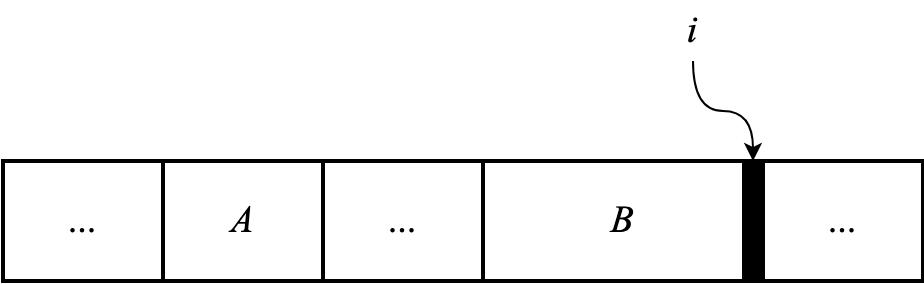
\includegraphics[scale=0.2]{img/max-sum}
%%       \begin{tikzpicture}[scale=0.8]
%%       \draw (0, 0) rectangle (1, 1) node [pos=.5] {...}
%%             (1, 0) rectangle (2, 1) node [pos=.5] {$A$}
%%             (2, 0) rectangle (3, 1) node [pos=.5] {...}
%%             (3, 0) rectangle (6, 1) node (rest) [pos=.5] {$B$}
%%             (6, 0) rectangle (7, 1) node [pos=.5] {...};
%%       \fill [black] (6, 0) rectangle (6.1, 1) node (ibar) [pos=.5] {};
%%       \draw (6, 2) node (i) {i};
%%       \draw[thick, ->] (i) edge [bend right] (ibar);
%%       \end{tikzpicture}
 \caption{$A$是目前找到的最大子序列和,$B$是以$i$结尾的子序列和。}
 \label{fig:max-sum-invariant}
\end{figure}

\btab{|l|l|r|}
\hline
最大和 & 以$i$结尾的子序列和 & 尚未扫描部分 \\
\hline
0 & 0 & $[3, -13, 19, -12, 1, 9, 18, -16, 15, -15]$ \\
3 & 3 & $[-13, 19, -12, 1, 9, 18, -16, 15, -15]$ \\
3 & 0 & $[19, -12, 1, 9, 18, -16, 15, -15]$ \\
19 & 19 & $[-12, 1, 9, 18, -16, 15, -15]$ \\
19 & 7 & $[1, 9, 18, -16, 15, -15]$ \\
19 & 8 & $[9, 18, -16, 15, -15]$ \\
19 & 17 & $[18, -16, 15, -15]$ \\
35 & 35 & $[-16, 15, -15]$ \\
35 & 19 & $[15, -15]$ \\
35 & 34 & $[-15]$ \\
35 & 19 & $[\ ]$\\
\hline
\etab

\begin{algorithmic}[1]
\Function{Max-Sum}{$V$}
  \State $A \gets 0, B \gets 0, n \gets |V|$
  \For{$i \gets 1$ to  $n$}
    \State $B \gets $ \Call{Max}{$B + V[i], 0$}
    \State $A \gets $ \Call{Max}{$A, B$}
  \EndFor
  \State \Return $A$
\EndFunction
\end{algorithmic}

我们也可以用叠加查找子序列最大和:$S_{max} = fst \circ foldr\ f\ (0, 0)$,其中$f$更新最大和:

\be
f\ x\ (S_m, S) = (S_m' = \max(S_m, S'), S' = \max(0, x + S))
\ee

\begin{Exercise}\label{ex:max-subsum}
\Question{修改最大子序列和的实现,返回对应最大和的子序列。}
\Question{本特利\cite{Bentley}给出了一个分而治之的方法求子数组最大和。复杂度为$O(n \log n)$。思路是将列表在中点分成两份。我们可以递归地找出前半部分的最大和,和后半部分的最大和,和跨越中点部分的最大和。实现这一方法。
}
\Question{在$m \times n$的二维整数矩阵中寻找子矩阵,使得各元素相加后的和最大。}
\end{Exercise}

\begin{Answer}[ref = {ex:max-subsum}]
\Question{修改最大子序列和的实现,返回对应最大和的子序列。

如果除了最大子序列和,还希望返回子序列,我们可以在fold过程中使用两对值$P_m$和$P$,每对值都包括子序列的和与子序列本身$(S, L)$。

\blre
max_s & = & fst \cdot foldr\ f\ ((0, [\ ]), (0, [\ ])) \\
\text{其中}: & & f\ x\ (P_m, (S, L)) = (P_m', P') \\
& & \text{在$f$中}:  P' = max((0, [\ ]), (x + S, x \cons L)), P_m' = max(P_m, P') \\
\elre
}
\Question{本特利\cite{Bentley}给出了一个分而治之的方法求子数组最大和。复杂度为$O(n \log n)$。思路是将列表在中点分成两份。我们可以递归地找出前半部分的最大和,和后半部分的最大和,和跨越中点部分的最大和。实现这一方法。

\begin{algorithmic}[1]
\Function{Max-Sum}{$A$}
  \If{$A = \phi$}
    \State \Return 0
  \ElsIf{$|A| = 1$}
    \State \Return \Call{Max}{$0, A[1]$}
  \Else
    \State $m \gets \lfloor \frac{|A|}{2} \rfloor$
    \State $a \gets$ \textproc{Max-From}(\Call{Reverse}{$A[1...m]$})
    \State $b \gets$ \Call{Max-From}{$A[m+1...|A|]$}
    \State $c \gets$ \Call{Max-Sum}{$A[1...m]$}
    \State $d \gets$ \Call{Max-Sum}{$A[m+1...|A|$}
    \State \Return \textproc{Max}($a+b, c, d$)
  \EndIf
\EndFunction
\Statex
\Function{Max-From}{$A$}
  \State $sum \gets 0, m \gets 0$
  \For{$i \gets 1$ to $|A|$}
    \State $sum \gets sum + A[i]$
    \State $m \gets $ \Call{Max}{$m, sum$}
  \EndFor
  \State \Return $m$
\EndFunction
\end{algorithmic}
复杂度存在递归关系$T(n) = 2T(n/2) + O(n)$。利用主定理可知复杂度为$O(n)$。
}

\Question{在$m \times n$的二维整数矩阵中寻找子矩阵,使得各元素相加后的和最大。

我们从矩阵中的第一行开始,每轮增加一行$[M[1, *], M[2, *], ..., M[i, *]]$。然后沿列把各行中的值加起来转换成一维向量:

\[
V = \left [ \sum_{j=1}^i M[1, j], \sum_{j=1}^i M[2, j], ..., \sum_{j=1}^i M[n, j] \right ]
\]

再使用本节中介绍的$maxsum$求出向量$V$中的最大和,并记录全局最大和。

\begin{Haskell}
maxSum = maximum . (map maxS) . acc . rows where
    rows = init . tails              -- exclude the empty row
    acc = concatMap (scanl1 (zipWith (+))) -- accumulated sum along columns
    maxS = snd . (foldl f (0, 0))    -- max sum in a vector
    f (m, s) x = let m' = max (m + x) 0
                     s' = max m' s in (m', s')
\end{Haskell}

其中\texttt{tails}的定义见\cref{ex:list-tails},\texttt{zipWith}的定义见\cref{sec:list-zipwith},\texttt{concatMap}的定义见\cref{sec:list-concatmap}。$scanl$和$foldl$类似,但它每次把结果都保存到一个列表中。$scanl1$是$scanl$的一个特殊情况,初始值是列表的第一个元素。

\[
\begin{array}{rcl}
scanl1\ f [\ ] & = & [\ ] \\
scanl1\ f (x \cons xs) & = & scanl\ f\ x\ xs \\
\end{array}
\]
其中:
\[
\begin{array}{rcl}
scanl\ f\ q\ [\ ] & = & [q] \\
scanl\ f\ (x \cons xs) & = & q : scanl\ f\ (f\ q\ x)\ xs \\
\end{array}
\]

对应的命令式例子程序如下:
\begin{Bourbaki}
K maxsum2([[K]] m) {
    Int n = length(m), k = length(m[0]) // number of row, col
    K maxs = 0            // max so far
    for i = 0 to n - 1 {
        xs = [0] * k
        for j = i to n - 1 {
            xs = [x + y for (x, y) in zip(xs, m[j])]
            maxs = max(maxs, maxsum1(xs))
        }
    }
    return maxs
}

K maxsum1([K] xs) {
    K s = 0 // max so far
    K m = 0 // max end here
    for x in xs {
        m = max(m + x, 0)
        s = max(m, s)
    }
    return s
}
\end{Bourbaki}
}
\end{Answer}

\section{字符串搜索}
字符串搜索是一类实用问题。所有文本编辑软件都带有字符串搜索功能。在基数树、前缀树中(第6章),我们利用特殊的数据结构进行搜索。我们也可以直接在字符串序列中进行搜索,如\cref{fig:strstr}所示\footnote{编程环境一般会提供一些逐一搜索工具,如C标准库中的\texttt{strstr},C++标准库中的\texttt{find},以及Java标准库中的\texttt{indexOf}。}。

\begin{figure}[htbp]
 \centering
 \subcaptionbox{偏移量$s = 4$,连续$q=4$个字符相同,但第5个字符不同。}{\input{img/strstr.tex}} \\
 \subcaptionbox{偏移到$s = 4 + 2 = 6$。}{\input{img/kmp.tex}}
 \caption{在文本“any ananthous ananym flower”中寻找“ananym”}
 \label{fig:strstr}
\end{figure}

%% \subsection{KMP算法}
\index{KMP} \index{Knuth-Morris-Pratt算法}

在文本$T$中搜索字符串$P$。如\cref{fig:strstr} (a)所示,在偏移量$s=4$时,逐一检查$P$和$T$中的字符。前4个相等,第5个在$P$中是y,但在$T$中是t。此时逐一比较立即终止,将$s$加1($P$向右移动1个位置)然后重新比较ananym和nantho……我们发现$s$的增量可以超过1。前两个字符an恰好是anan的后缀。我们可以将$s$增加2($P$向右移动2),如\cref{fig:strstr} (b)所示。我们复用了此前已经比较过4个字符的信息,跳过了无需比较的位置。高德纳、莫里斯、普拉特根据这一想法给出了一个高效的字符串匹配算法\cite{kmp},人们把三人名字的首字母合在一起,称作KMP算法。

记文本$T$中前$k$个字符组成的串为$T_k$($T$的$k$个字符前缀)。为了尽可能多地把$P$向右移动$s$个位置,我们需要利用已成功匹配的$q$个字符。如\cref{fig:kmp-fallback}所示,若$P$可向右移动,则一定存在某个$k$,使得$P$中的前$k$个字符和前缀$P_q$的最后$k$个字符相同。也就是说,前缀$P_k$同时是$P_q$的后缀。定义空串“”是任何串的前缀和后缀,则总存在最小的$k=0$。我们要找到同时既是前缀又是后缀的最大$k$。定义\textbf{前缀函数}$\pi(q)$,它告诉我们当第$q+1$个字符不匹配时应该回退的位置\cite{CLRS}。

\begin{figure}[htbp]
 \centering
 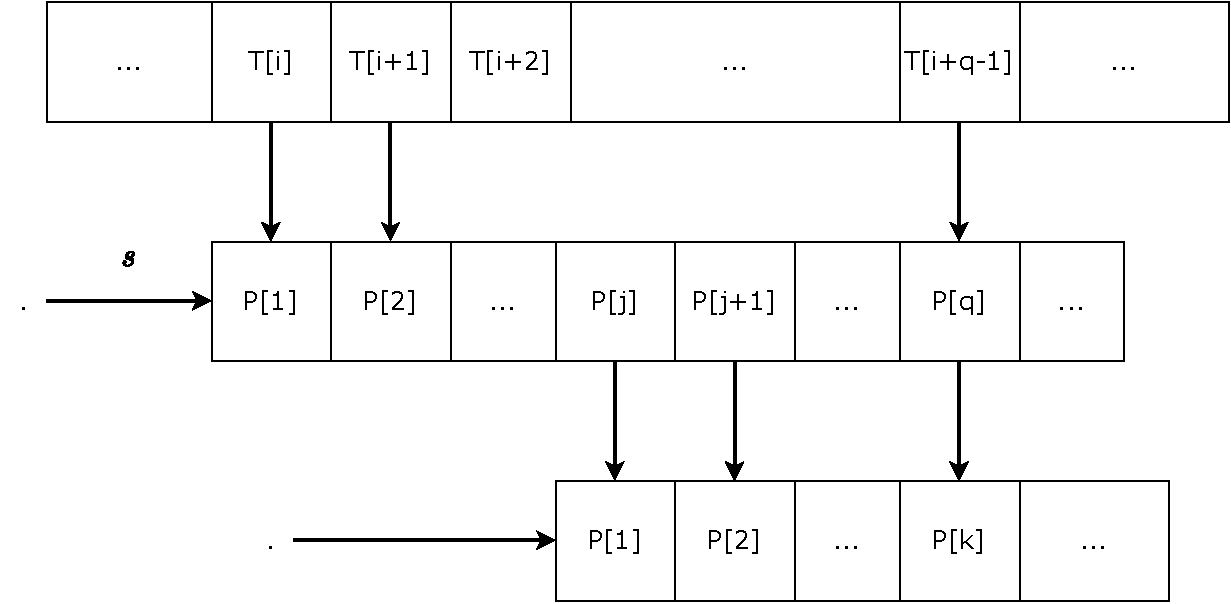
\includegraphics[scale=0.5]{img/kmp-fallback}
 \caption{$P_k$同时是$P_q$的前缀和后缀}
 \label{fig:kmp-fallback}
\end{figure}

\be
\pi(q) = \max \{ k | 0 \leq k < q, \text{且} P_k \text{是} P_q \text{的后缀}\}
\label{eq:prefix-function}
\ee

当在文本$T$中偏移$s$匹配$P$时,若前$q$个字符相同,而下一个不同,我们通过$q' = \pi(q)$找到一个回退的位置$q'$。重新比较$P[q']$和文本:

\begin{algorithmic}[1]
\Function{KMP}{$T, P$}
  \State $\pi \gets $ \Call{Build-Prefixes}{$P$}
  \State $n \gets |T|, m \gets |P|, q \gets 0$
  \For{$i \gets 1$ to $n$}
    \While{$q > 0$ 且 $P[q+1] \neq T[i]$}
      \State $q \gets \pi(q)$
    \EndWhile
    \If{$P[q+1] = T[i]$}
      \State $q \gets q + 1$
    \EndIf
    \If{$q = m$}
      \State 位置$i - m$是一个解
      \State $q \gets \pi(q)$ \Comment{寻找更多的匹配位置}
    \EndIf
  \EndFor
\EndFunction
\end{algorithmic}

直接利用\cref{eq:prefix-function}构造$\pi(q)$并不实用,我们进一步复用信息,构造前缀函数。如果第一个字符就不匹配,此时最长前缀同时也是后缀的显然是空串:$\pi(1) = 0$。即:$P_k = P_0 = [\ ]$。当扫描到$P$中第$q$个字符时,前缀函数值$\pi(i)$,$i = 1, 2, ..., q-1$都已算好,并且目前最长的前缀$P_k$同时也是$P_{q-1}$的后缀。如\cref{fig:kmp-prefix-func}所示,若$P[q] = P[k+1]$,则找到了一个更大的$k$,我们将$k$的最大值加一;否则$P[q] \neq P[k + 1]$,我们利用$\pi(k)$回退到一个较短的$P_{k'}$,其中$k' = \pi(k)$,然后比较这个新前缀的下一个字符是否和第$q$个字符相等。重复这一步骤,直到$k$变成0(空串),或者和第$q$个字符相等。下表给出了ananym的前缀函数值,$k$列是满足\cref{eq:prefix-function}的最大值。

\begin{figure}[htbp]
 \centering
 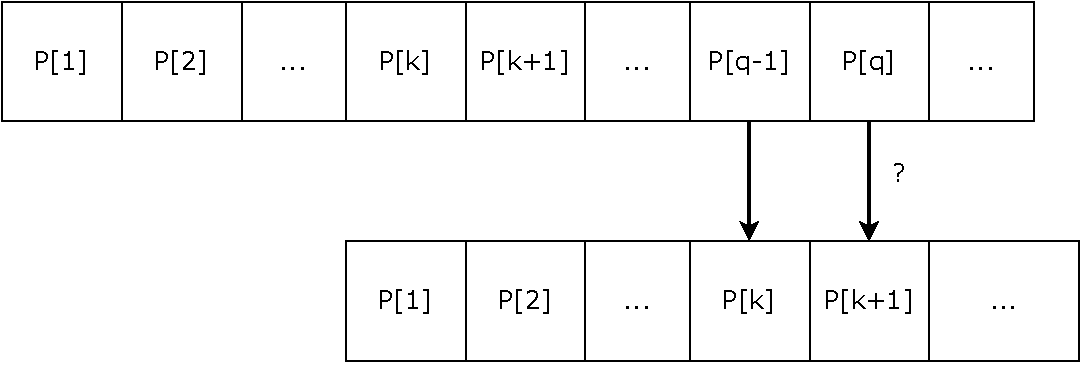
\includegraphics[scale=0.5]{img/kmp-prefix-func}
 \caption{$P_k$是$P_{q-1}$的后缀,比较$P[q]$和$P[k+1]$}
 \label{fig:kmp-prefix-func}
\end{figure}

\btab{|c|r|c|l|}
\hline
$q$ & $P_q$ & $k$ & $P_k$ \\
\hline
1 & a & 0 & ``'' \\
2 & an & 0 & ``'' \\
3 & ana & 1 & a \\
4 & anan & 2 & an  \\
5 & anany & 0 & ``'' \\
6 & ananym & 0 & ``'' \\
\hline
\etab

\begin{algorithmic}[1]
\Function{Build-Prefixes}{$P$}
  \State $m \gets |P|, k \gets 0$
  \State $\pi(1) \gets 0$
  \For{$q \gets 2$ to $m$}
    \While{$k > 0$ 且 $P[q] \neq P[k+1]$}
      \State $k \gets \pi(k)$
    \EndWhile
    \If{$P[q] = P[k+1]$}
      \State $k \gets k + 1$
    \EndIf
    \State $\pi(q) \gets k$
  \EndFor
  \State \Return $\pi$
\EndFunction
\end{algorithmic}

KMP对待搜索串预处理,构建前缀函数的分摊复杂度为$O(m)$\cite{CLRS}。搜索本身的分摊复杂度是$O(n)$。总体分摊复杂度为$O(m + n)$,并需要$O(m)$空间记录前缀函数值。待搜索串的形式并不影响KMP算法的性能。考虑在“aaa...a”($n$个)中搜索长为$m$的子串“aaa...ab”。第$m$个字符不匹配,我们只能回退一个字符,并且此后不断回退1个字符。即使在这种情况下,KMP算法依旧是线性时间的。

% 伯德给出了一个纯函数式的KMP算法(\cite{fp-pearls}第17章)。

%% \subsection{鲍耶-摩尔算法}
%% \index{Boyer-Moore算法}

%% 鲍耶-摩尔在1977年给出了一种字符串匹配算法\cite{boyer-moore}。如\cref{fig:bad-char}所示,即使按照KMP算法向右平移2仍然匹配失败。待查找字符串ananym长度为6,最后一个字符对应文本中的h。而h根本没有出现在待搜索串中。我们据此可以直接向右平移6。这一规则叫做\textbf{不良字符规则}:对$P$进行预处理。设字符集为$\Sigma$,找到所有不在$P$中的不良字符$B = {c | c \in \Sigma, c \notin P}$。扫描时遇到不良字符就向右移动距离$|P|$。如果不匹配的字符$c \in P$,为了避免漏掉解,我们只能向右移动较短的距离重新搜索,如\cref{fig:good-char}所示。字符$c$可能在$P$中出现多次,从左向右位于$p_1, p_2, ..., p_i$。为避免遗漏,我们用最后一个位置$p_i$计算平移的距离:

%% \begin{figure}[htbp]
%%  \centering
%%  \includegraphics[scale=0.6]{img/strstr}
%%  \caption{h没有出现在$P$中,应向右侧至少平移6。}
%%  \label{fig:bad-char}
%% \end{figure}

%% \be
%% s = |P| - p_i
%% \label{eqn:BMH-shift}
%% \ee

%% \begin{figure}[htbp]
%%  \centering
%%  \subcaptionbox{e $\neq$ p,但p $\in P$。}{\includegraphics[scale=0.5]{img/good-char}} \\
%%  \subcaptionbox{向右平移2。}{\includegraphics[scale=0.5]{img/good-char-2}}
%%  \caption{不匹配的字符$c \in P$。}
%%  \label{fig:good-char}
%% \end{figure}

%% 我们跳过$c$出现在$P$末尾的情况,此时$p_i = |P|$,平移$s = 0$。由于$s$是相对$P$末尾计算的,从右向左扫描时,一旦匹配失败,我们需要检查待末尾字符$r$在文本中的对应的字符是在不良字符集$B$中,如\cref{fig:good-char-2}。

%% \begin{figure}[htbp]
%%  \centering
%%  \subcaptionbox{}{\includegraphics[scale=0.5]{img/good-char-3}}
%%  \subcaptionbox{}{\includegraphics[scale=0.5]{img/good-char-4}}
%%  \caption{从右向左检查到i $\neq$ a,用末尾字符e计算平移$s = 6$(e在$P$中出现两次,第二次在末尾,此时$s=0$,需要跳过)。}
%%  \label{fig:good-char-2}
%% \end{figure}

%% 仅使用不良字符规则就可得到简单快速的查找算法,称为鲍耶-摩尔-霍斯普尔算法\cite{boyer-moore-horspool}:

%% \begin{algorithmic}[1]
%% \Procedure{Boyer-Moore-Horspool}{$T, P$}
%%   \State $m \gets |P|, n \gets |T|$
%%   \For{each $c \in \Sigma$}
%%     \State $\pi[c] \gets m$ \Comment{初始化所有平移距离为$m = |P|$}
%%   \EndFor
%%   \For{$i \gets 1$ to $m - 1$} \Comment{跳过末尾位置}
%%     \State $\pi[P[i]] \gets m - i$ \Comment{定义\cref{eqn:BMH-shift}}
%%   \EndFor
%%   \State $s \gets 0$
%%   \While{$s + m \leq n$}
%%     \State $i \gets m$
%%     \While{$i \geq 1$ 且 $P[i] = T[s+i]$} \Comment{从右向左扫描}
%%       \State $i \gets i - 1$
%%     \EndWhile
%%     \If{$i < 1$}
%%       \State 位置$s$是一个解
%%       \State $s \gets s + 1$ \Comment{寻找下一个解}
%%     \Else
%%       \State $s \gets s + \pi[T[s + m]]$
%%     \EndIf
%%   \EndWhile
%% \EndProcedure
%% \end{algorithmic}

%% 首先将平移表$\pi$的所有值都初始化为$m = |P|$。然后从左向右处理$P$,更新平移距离$\pi(P[i]) = m - i$。如果某个字符出现多次,后面值将覆盖此前的值。将文本和$P$的左侧对齐开始查找。但每个对齐位置$s$,我们都从右向左扫描,如果不匹配就查找$\pi$并移动相应的距离。我们首先用$O(|\Sigma| + |P|)$的时间构造平移表$\pi$。如果字符集不大,复杂度主要由$P$和文本长度决定。最坏情况下,文本和$P$中的字符相同,例如在文本“aa......a”($n$个)中搜索“aa...a”($m$个)。复杂度为$O(mn)$。当$P$较长并且有常数个解时,复杂度为线性时间。

%% 考虑在文本bbbababbabab...中搜索abbabab,如\cref{fig:bad-char-2}所示。根据不良字符规则,应向右侧平移2。我们可以平移更长的距离。考虑已从右向左成功匹配了6个字符bbabab,由于ab既是$P$的前缀也是已匹配部分的后缀,我们向右平移对齐这个后缀,如\cref{fig:good-suffix-case1-1}所示。这类似于KMP中的预处理。但并不能总跳过这样多的字符。考虑如\cref{fig:good-suffix-case2-1}所示的例子,已匹配了bab。虽然前缀ab也是bab的后缀,但却不能平移这么远。因为bab也在其它位置出现过($P$中第3个字符的位置)。为了避免漏掉解,只能向右平移2。

%% \begin{figure}[htbp]
%%  \centering
%%  \subcaptionbox{}{\includegraphics[scale=0.5]{img/bad-char-1}}
%%  \subcaptionbox{}{\includegraphics[scale=0.5]{img/bad-char-2}}
%%  \caption{不良字符规则:向右平移2,对齐字符b。}
%%  \label{fig:bad-char-2}
%% \end{figure}

%% \begin{figure}[htbp]
%%  \centering
%%  \includegraphics[scale=0.5]{img/good-suffix-case1-1}
%%  \caption{由于前缀ab也是已匹配部分的后缀,向右平移对齐ab}
%%  \label{fig:good-suffix-case1-1}
%% \end{figure}

%% \begin{figure}[htbp]
%%  \centering
%%  \subcaptionbox{}{\includegraphics[scale=0.5]{img/good-suffix-case2-1}}
%%  \subcaptionbox{}{\includegraphics[scale=0.5]{img/good-suffix-case2-2}}
%%  \caption{bab也在$P$中其它位置出现(第3~5个字符)。只能向右平移2。}
%%  \label{fig:good-suffix-case2-1}
%% \end{figure}

%% 以上两种情况组成了\textbf{良好后缀规则},如\cref{fig:good-suffix-cases}所示。下面两种情况之一可向右平移。我们优先使用规则2然后再应用规则1。

%% \begin{enumerate}
%% \item 如果已匹配部分的某个后缀也是$P$的前缀,并且这一后缀不出现在$P$的其它位置,将$P$向右平移对齐这一前缀;
%% \item 如果已匹配部分的某个后缀也出现在$P$的其它位置,将$P$向右侧平移,对齐最右侧出现的位置。
%% \end{enumerate}

%% \begin{figure}[htbp]
%%  \centering
%%  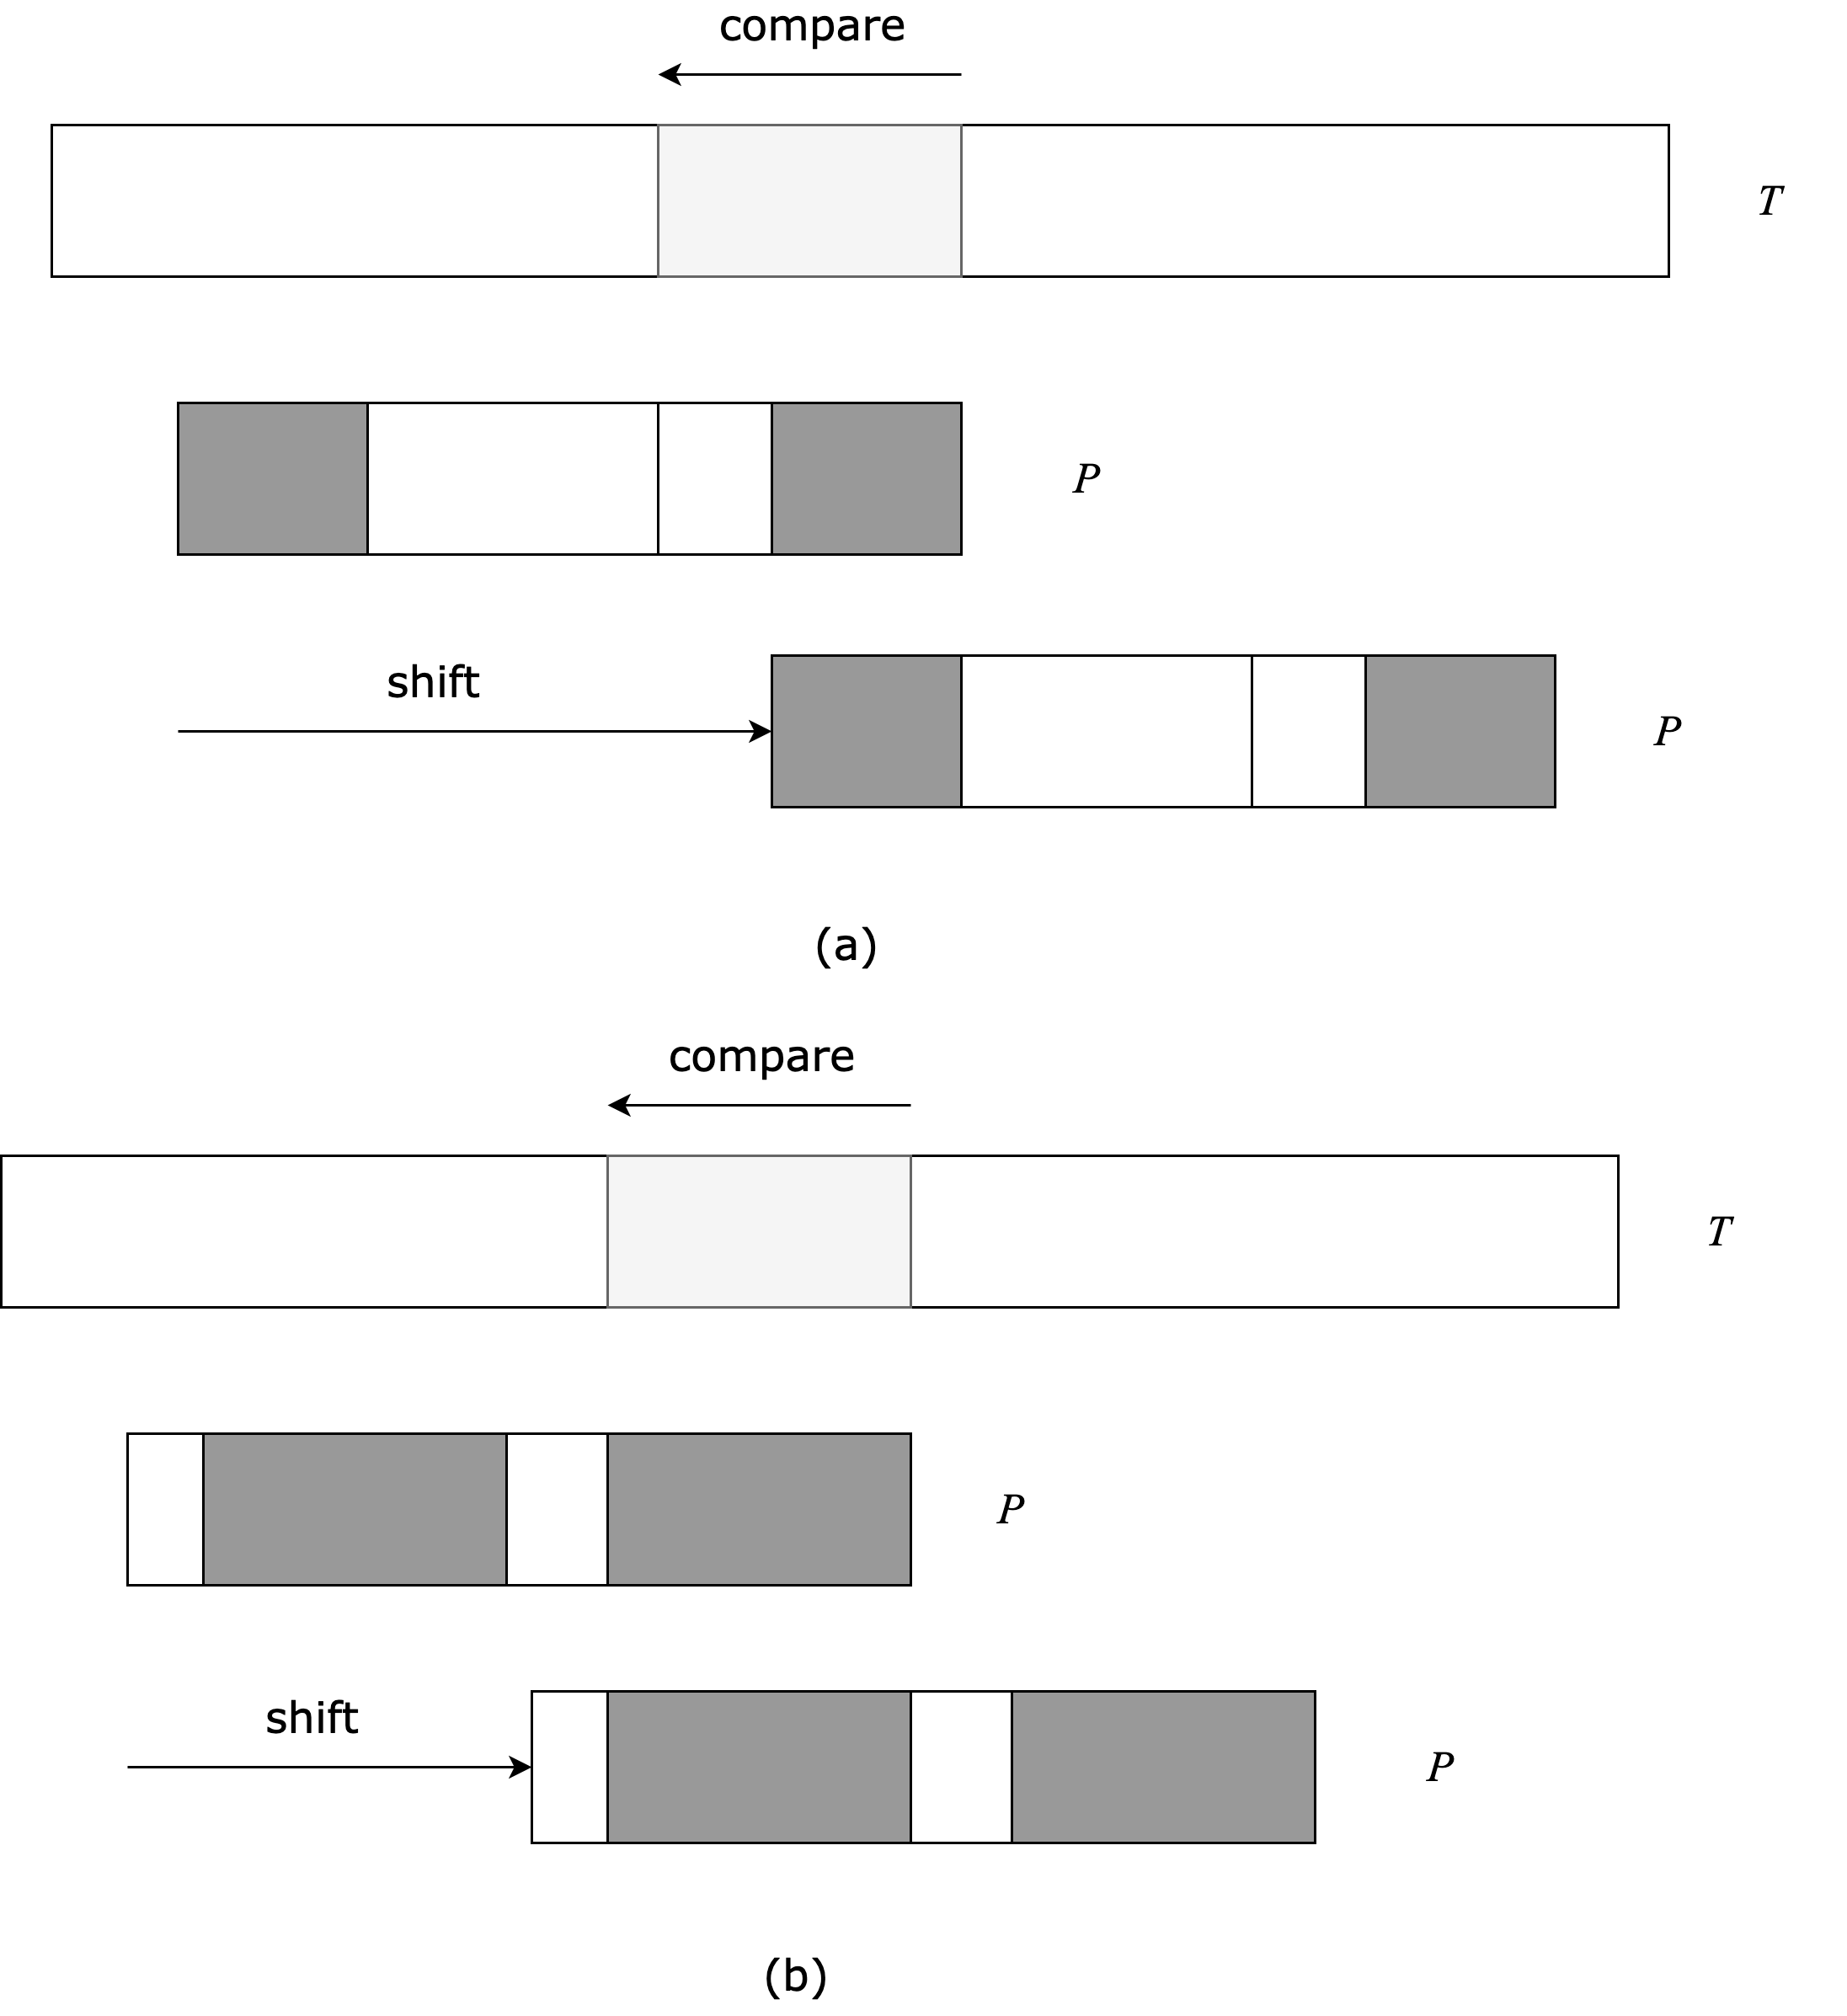
\includegraphics[scale=0.5]{img/BM-good-suffix-rule}
%%  \caption{$T$中浅灰色是已匹配部分,和$P$中深灰色的部分相同。(a) 情况1,已匹配子串中有一部分也是$P$的前缀;(b) 情况2,匹配部分的后缀,也出现在$P$中其它位置。}
%%  \label{fig:good-suffix-cases}
%% \end{figure}

%% 良好后缀规则仅依赖于$P$,可以在搜索前预处理。记$P$中从第$i$个字符开始的后缀为$\overline{P_i} = P[i...m]$,其中$m = |P|$。对规则1,从右向左扫描检查$P$的每个后缀:$\overline{P_m}$, $\overline{P_{m-1}}$, ...,  $\overline{P_2}$是否是$P$的前缀。对规则2,从左向右扫描$P$的每个前缀:$P_1$, $P_2$, ..., $P_{m-1}$,检查它的最长后缀是否也是$P$的后缀:

%% \begin{algorithmic}[1]
%% \Function{Good-Suffix}{$P$}
%%   \State $m \gets |P|$
%%   \State $\pi_s \gets [0, 0, ..., 0]$ \Comment{$m$个}
%%   \State $l \gets 0$                  \Comment{空串}
%%   \For{$i \gets m-1$ down-to $1$}     \Comment{从右向左扫描规则1}
%%     \If{$\overline{P_i} \sqsubset P$} \Comment{$A \sqsubset B$:$A$是$B$的前缀}
%%       \State $l \gets i$
%%     \EndIf
%%     \State $\pi_s[i] \gets l$
%%   \EndFor
%%   \For{$i \gets 1$ to $m$} \Comment{从左向右扫描规则2}
%%     \State $s \gets$ \Call{Suffix-Length}{$P_i$}
%%     \If{$s \neq 0$ 且 $P[i - s] \neq P[m - s]$}
%%       \State $\pi_s[m - s] \gets m - i$
%%     \EndIf
%%   \EndFor
%%   \State \Return $\pi_s$
%% \EndFunction
%% \end{algorithmic}

%% 为了构造良好后缀规则表$\pi_s$,首先从右向左检查$P$的每个后缀$\overline{P_i}$是否是$P$的前缀并记录。然后从左向右检查$P$的每个前缀,调用函数\textproc{Suffix-Length}($P_i$)找出同时是$P$前缀的后缀的最长长度$s$,若$s \neq 0$,则修改表格$\pi_s$中倒数第$s$项的值。为避免重复找到已匹配的后缀,需要检查$P[i - s]$和$P[m - s]$是否相等。\textproc{Suffix-Length}的实现如下:

%% \begin{algorithmic}[1]
%% \Function{Suffix-Length}{$P_i$}
%%   \State $m \gets |P|, j \gets 0$
%%   \While{$P[m - j] = P[i - j]$ 且 $j < i$}
%%     \State $j \gets j + 1$
%%   \EndWhile
%%   \State \Return $j$
%% \EndFunction
%% \end{algorithmic}

%% 可以同时应用不良字符规则和良好后缀规则,比较并选择较大的平移值:

%% \begin{algorithmic}[1]
%% \Function{Boyer-Moore}{$T, P$}
%%   \State $n \gets |T|, m \gets |P|$
%%   \State $\pi_b \gets$ \Call{Bad-Character}{$P$}
%%   \State $\pi_s \gets$ \Call{Good-Suffix}{$P$}
%%   \State $s \gets 0$
%%   \While{$s + m \leq n$}
%%     \State $i \gets m$
%%     \While{$i \geq 1$ 且 $P[i] = T[s + i]$}
%%       \State $i \gets i - 1$
%%     \EndWhile
%%     \If{$i < 1$}
%%       \State 位置$s$是一个解
%%       \State $s \gets s + 1$ \Comment{继续寻找下一个解}
%%     \Else
%%       \State $s \gets s + max(\pi_b[T[s + m]], \pi_s[i])$
%%     \EndIf
%%   \EndWhile
%% \EndFunction
%% \end{algorithmic}

%% 在最坏的情况下,只有当$P$不出现在文本中时复杂度才是$O(n+m)$\cite{boyer-moore}。如果$P$出现,则复杂度为$O(nm)$。伯德给出了算法的一种纯函数式实现(\cite{fp-pearls}第16章)。

\section{解的搜索}

在早期人工智能阶段,人们发展出了许多方法搜索解。不同于字符串匹配,解并不一定直接存在于一个候选答案集中。往往需要一边构造解一边尝试。某些问题可解,某些问题无解。也可能存在多个解。例如存在多条走出迷宫的路线。人们还需要求出某种意义下的最优解。

\subsection{深度优先和广度优先搜索}
\index{DFS} \index{深度优先搜索}
深度优先搜索(DFS)和广度优先搜索(BFS)常被叫做“图搜索”算法。我们简单介绍这两种搜索算法而略过图的概念。

\subsubsection{迷宫}
\index{迷宫问题}
走迷宫是一类历史悠久的趣题。有窍门说:当遇到分叉时总向右转。这个方法有缺陷,如\cref{fig:maze-loop}所示,不断向右会绕着中心的大方块转圈。存在多个选项时,决策直接影响到最终的解。童话故事提供了一种思路:携带一块面包进入迷宫。遇到岔路时任选一条道路,并留下一小块面包屑记录下这次尝试。遇到了死胡同就沿着留下的面包屑向回走到上次做出选择的地方,然后换一条路。一旦发现地上已经有面包屑了,就说明我们进入了循环,必须回退并重新尝试。不断这样的“尝试——检查”,我们要么最终走出迷宫,要么退回起点(无解)。我们用$m \times n$的矩阵$M$描述迷宫,元素值为0、1,表示是否有路。\cref{fig:maze-loop}的迷宫可以用下面的矩阵定义:

\begin{figure}[htbp]
 \centering
 \subcaptionbox{迷宫}{\includegraphics[scale=0.3]{img/maze}}
 \subcaptionbox{一直右转陷入循环}{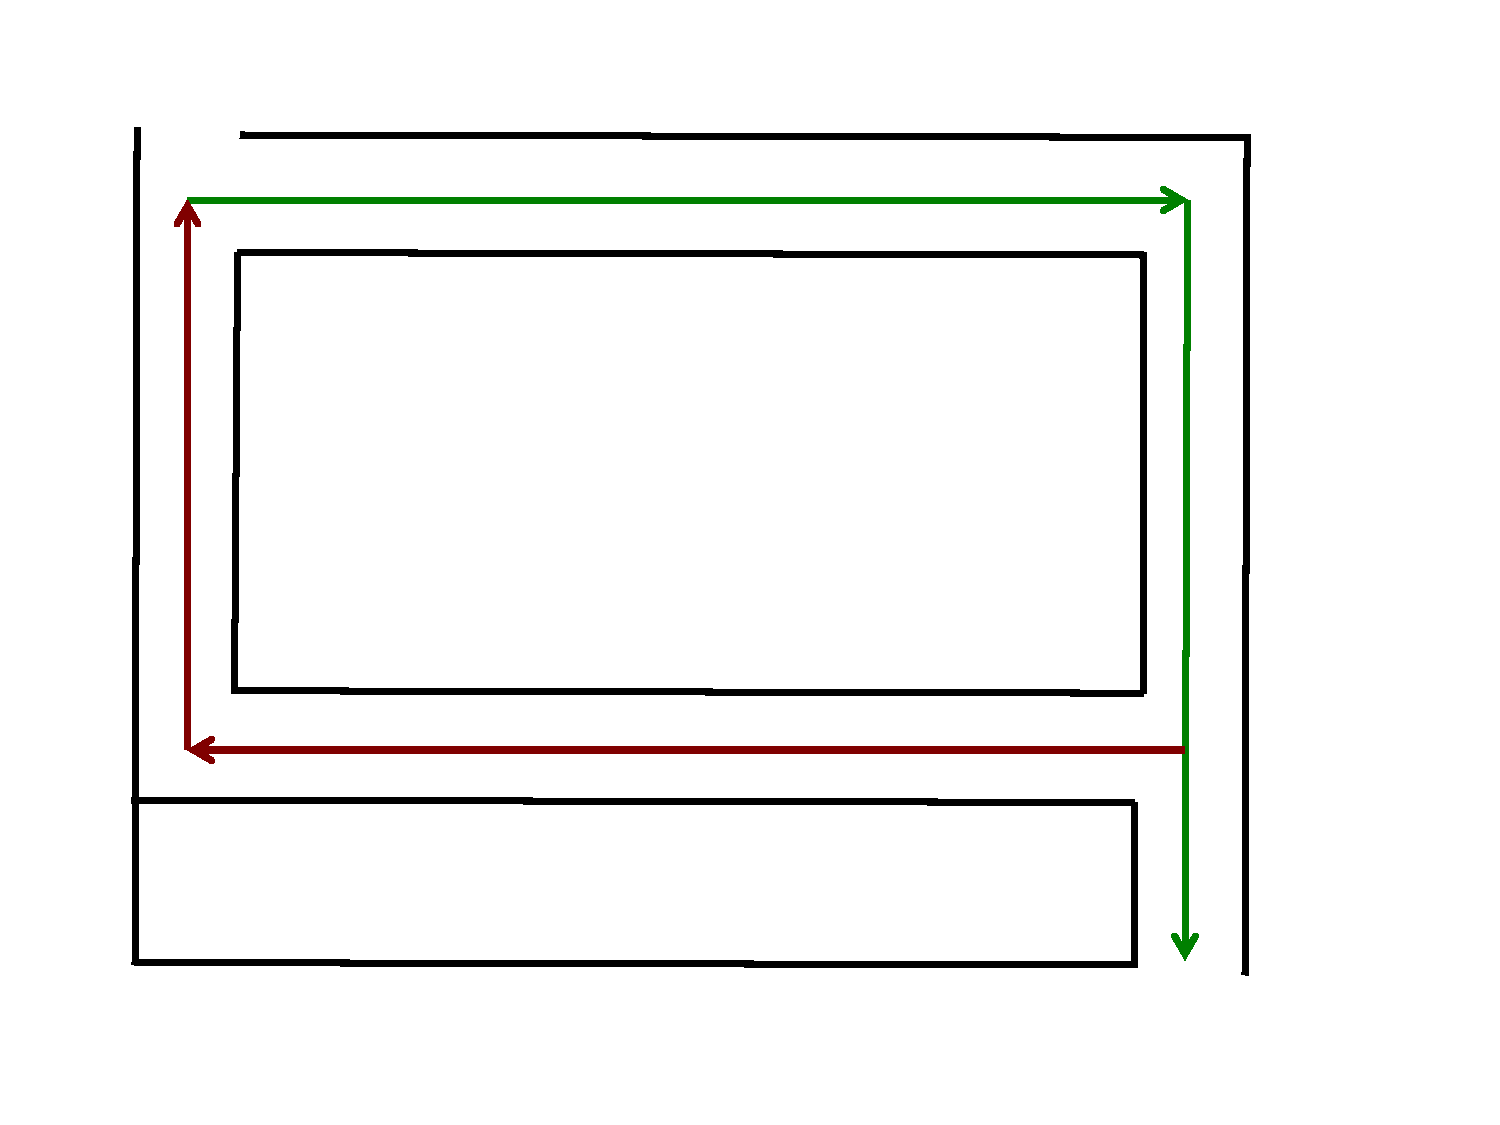
\includegraphics[scale=0.6]{img/maze-loop}}
 \caption{迷宫}
 \label{fig:maze-loop}
\end{figure}

\[
M = \begin{matrix}
0 & 0 & 0 & 0 & 0 & 0 \\
0 & 1 & 1 & 1 & 1 & 0 \\
0 & 1 & 1 & 1 & 1 & 0 \\
0 & 1 & 1 & 1 & 1 & 0 \\
0 & 1 & 1 & 1 & 1 & 0 \\
0 & 0 & 0 & 0 & 0 & 0 \\
1 & 1 & 1 & 1 & 1 & 0
\end{matrix}
\]

给定起点$s=(i, j)$、终点$e=(p, q)$,我们要找出所有从$s$到$e$的通路。我们先找出所有和$s$连通的相邻点,对每个邻点$k$,递归找出从$k$到$e$所有路径。然后将通路$s$-$k$连接到每个从$k$到$e$的路径前。我们需要留下一些“面包屑”标记以避免重复。我们用一个列表$P$记录走过的所有位置。每次检查此列表,只尝试新路径。

\be
\textit{solveMaze}\ M\ s\ e = \textit{solve}\ s\ [[\ ]]
\label{eq:solve-maze-reversed}
\ee

其中:

\be
\textit{solve}\ s\ P = \begin{cases}
  s = e: & map\ (\textit{reverse} \circ (s:))\ P \\
  \text{否则}: & \textit{concat}\ [\textit{solve}\ k\ (map\ (s:)\ P) | k \gets adj\ s, k \notin P] \\
  \end{cases}
\ee

$P$中保存的路径是逆序的,我们需要最终通过\textit{reverse}将其反转。$adj\ p$找出$p$相连通的邻点:水平、垂直方向上相邻为0的点:

\be
\begin{array}{ll}
adj\ (x, y) = [(x', y') | & (x', y') \gets [(x-1, y), (x+1, y), (x, y-1), (x, y+1)], \\
 & 1 \leq x' \leq m, 1 \leq y' \leq n, M_{x' y'} = 0\} \\
\end{array}
\ee

这是一种穷举解法,搜索所有路径。为了走出迷宫,只需要找到一条路径。我们需要某种数据结构保存“面包屑”,记录此前做出的决策。我们总在最新决策基础上搜索通路,这是后进先出的顺序。可以用一个栈来实现。开始时,栈中只有起点$[s]$。将其弹出,找出和$s$连通的点,例如$a$、$b$……将可能的路径$[a, s]$、$[b, s]$入栈。接下来将路径$[a, s]$弹出,检查和$a$连通的点。然后把所有3步可达的路径入栈。重复这一过程。栈中记录了一条条逆序路径:从可达的最远位置反向到起点,如\cref{fig:dfs-stack}所示。当栈变为空时,我们已尝试了所有的可能,搜索结束;否则弹出栈顶的候选路径,扩展未曾走过的连通邻点,然后入栈。

\begin{figure}[htbp]
 \centering
 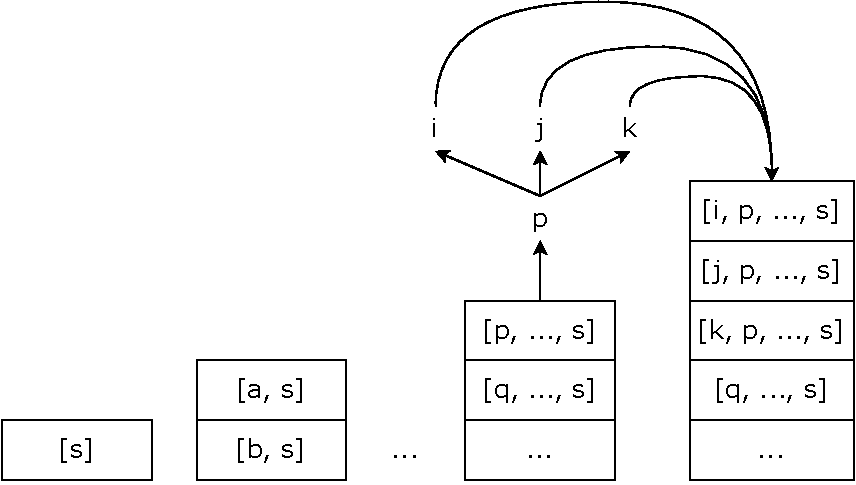
\includegraphics[scale=0.5]{img/dfs-stack}
 \caption{用栈记录路径}
 \label{fig:dfs-stack}
\end{figure}

\be
\textit{solveMaze}\ M\ s\ e = \textit{solve}\ [[s]]
\ee

其中:

\be
\begin{array}{rcl}
\textit{solve}\ [\ ] & = & [\ ] \\
\textit{solve}\ ((p \cons ps) \cons cs) & = & \begin{cases}
  c = e: & \textit{reverse}\ (p \cons ps) \\
  ks = [\ ]: & \textit{solve}\ cs, \text{其中}\ ks = filter\ (\notin ps)\ (adj\ p) \\
  ks \neq [\ ]: & \textit{solve}\ ((map\ (:p \cons ps)\ ks) \doubleplus cs)
  \end{cases}
\end{array}
\ee

对应的迭代实现如下:

\begin{algorithmic}[1]
\Function{Solve-Maze}{$M, s, e$}
  \State $S \gets [s], L = [\ ]$
  \While{$S \neq [\ ]$}
    \State $P \gets$ \Call{Pop}{$S$}
    \State $p \gets$ \Call{Last}{$P$}
    \If{$e = p$ }
      \State \Call{Add}{$L, P$}   \Comment{找到一个解}
    \Else
      \For{each $k$ in \Call{Adjacent}{$M, p$}}
        \If{$k \notin P$}
          \State \Call{Push}{$S, P \doubleplus [k]$}
        \EndIf
      \EndFor
    \EndIf
  \EndWhile
  \State \Return $L$
\EndFunction
\end{algorithmic}

每步有上下左右4个选项可能入栈,并且都在回溯时检查。复杂度看似是$O(4^n)$,其中$n$是路径长度。实际复杂度不会这样大,我们跳过了已走的位置。最坏情况下,所有可达点都恰好被访问过一次,复杂度为$O(n)$,其中$n$是连通点的数量。由于使用了栈来保存路径,空间复杂度为$O(n^2)$。

\begin{Exercise}\label{ex:dfs-maze}
\Question{使用栈来找出迷宫问题的所有解。}
\end{Exercise}

\begin{Answer}[ref = {ex:dfs-maze}]
\Question{使用栈来找出迷宫问题的所有解。

\begin{Haskell}
dfsSolveAll m from to = map reverse $ solve [[from]] [] where
    solve [] ss = ss
    solve (c@(p:path):cs) ss
        | p == to = solve cs (c:ss) -- find a solution, go on search
        | otherwise = let os = filter (`notElem` path) (adjacent p) in
                          if os == [] then solve cs ss
                          else solve ((map (:c) os) ++ cs) ss
    adjacent (x, y) = [(x', y') |
           (x', y') <- [(x-1, y), (x+1, y), (x, y-1), (x, y+1)],
           inRange (bounds m) (x', y'), m ! (x', y') == 0]
\end{Haskell}

对应的命令式程序
\begin{Bourbaki}
[[(Int, Int)]] solve([[Int]] m, (Int, Int) src, (Int, Int) dst) {
    [[(Int, Int)]] stack = [[src]]
    [[(Int, Int)]] s = []
    while stack != [] {
        path = stack.pop()
        if last(path) == dst {
            s.append(path)
        } else {
            for p in adjacent(m, last(path)) {
                if not p in path then stack.append(path + [p])
            }
        }
    }
    return s
}

[(Int, Int)] adjacent([[(Int, Int)]] m, (Int x, Int y)) {
    [(Int, Int)] ps = []
    for (dx, dy) in [(0, 1), (0, -1), (1, 0), (-1, 0)] {
        Int x1 = x + dx, y1 = y + dy
        if 0 <= x1 < len(m[0]) and 0 <= y1 < len(m)
           and m[y][x] == 0 then ps.append((x1, y1))
    }
    return ps
}
\end{Bourbaki}
}
\end{Answer}

\subsubsection{八皇后问题}
\index{八皇后问题}

虽然国际象棋历史悠久,但直到1848年贝策尔(Max Bezzel)才提出八皇后趣题\cite{wiki-8-queens}。皇后威力巨大,可以攻击同一行、列、斜线上的任意棋子。如何在棋盘上摆下八个皇后,而她们之间不互相攻击。\cref{fig:8-queens-puzzle} (a)描述了皇后可以攻击到的范围。\cref{fig:8-queens-puzzle} (b)给出了八皇后问题的某一种解。

\begin{figure}[htbp]
 \centering
 \subcaptionbox{国际象棋中的皇后}{\includegraphics[scale=1]{img/queen}}
 \subcaptionbox{一种解}{\includegraphics[scale=1]{img/queens-example}}
 \caption{八皇后问题}
 \label{fig:8-queens-puzzle}
\end{figure}

在64个格子中放入8个皇后,共有$P^8_{64}$种排列,约为$4 \times 10^{10}$。每行、列只能摆放1个皇后,一个解的布局必然是$[1,2,3,4,5,6,7,8]$的某种排列。例如布局$[6,2,7,1,3,5,8,4]$表示第一行的皇后放在第6列;第二行的皇后摆在第2列上……第8行的皇后摆在第4列。这样我们只需要检查$8! = 40320$种布局。从第一行开始逐一摆放皇后。第一个皇后有8种摆法(八列中的某一列)。摆放第二行的皇后时,由于可能和第一个皇后相互攻击,需要避开某些列。对于第$i$行的皇后,找到8列中不被前$i-1$个皇后攻击的位置。如果8个位置都不能摆放,我们就回退调整以前$i-1$个皇后。全部8个皇后都成功放入棋盘后,就找到了一个解。为了找出所有解,我们记录下这一布局,然后继续检查其它可能的列并进行必要的回溯。我们用一个栈和一个列表启动搜索:$solve\ [[\ ]]\ [\ ]$

\be
\begin{array}{rcl}
solve\ [\ ]\ s & = & s \\
solve\ (c \cons cs)\ s & = & \begin{cases}
  |c| = 8: & solve\ cs\ (c \cons s) \\
  \text{否则}: & solve\ ( [ x \cons c | x \gets [1..8], x \notin c, \textit{safe}\ x\ c] \doubleplus cs)\ s
  \end{cases}
\end{array}
\ee

若栈为空,我们已经尝试所有可能,$s$记录了所有找到的解;若栈顶布局$c$长度为8,我们找到了一个解。将其记录到$s$中,然后继续查找;若$|c| < 8$,我们从8列中找出尚未被占的列($x \notin c$),同时不能被斜线上的其它皇后攻击(通过\textit{safe} $x\ c$)。可行的布局入栈用于此后的搜索。

\be
\textit{safe}\ x\ c = \forall (i, j) \gets zip\ (\textit{reverse}\ c)\ [1, 2, ...]\ \text{有}: |x - i| \neq |y - j|, \text{其中}: y = 1 + |c|
\ee

\textit{safe}检查第$y = 1 + |c|$行,$x$列的皇后是否和$c$中任何皇后成对角线。若$c = [i_{y-1}, i_{y-2}, ..., i_1]$是前$y-1$个皇后所在的列,我们将$c$反转,并和1, 2, ...组成每个皇后的坐标:$[(i_1, 1), (i_2, 2), ..., (i_{y-1}, y-1)]$。然后判断每个$(i, j)$是否和位置$(x, y)$构成对角线:$|x - i| \neq |y - j|$。这一实现是尾递归的,可以消除递归优化为迭代实现:

\begin{algorithmic}[1]
\Function{Solve-Queens}{}
  \State $S \gets [[\ ]]$
  \State $L \gets [\ ]$ \Comment{保存解}
  \While{$S \neq [\ ]$}
    \State $A \gets$ \Call{Pop}{$S$} \Comment{$A$是某一中间布局}
    \If{$|A|=8$}
      \State \Call{Add}{$L, A$}
    \Else
      \For{$i \gets 1$ to $8$}
        \If{\Call{Valid}{$i, A$}}
          \State \Call{Push}{$S, A \doubleplus [i]$}
        \EndIf
      \EndFor
    \EndIf
  \EndWhile
  \State \Return $L$
\EndFunction
\Statex
\Function{Valid}{$x, A$}
  \State $y \gets 1 + |A|$
  \For{$i \gets 1$ to $|A|$}
    \If{$x = A[i]$ 或 $|y-i| = |x - A[i]|$}
      \State \Return False
    \EndIf
  \EndFor
  \State \Return True
\EndFunction
\end{algorithmic}

虽然每个皇后有8列选择,但只尝试尚未被占的列。总共检查15720种情况,远远小于$8^8 = 16777216$种可能\cite{wiki-8-queens}。由于正方形棋盘水平、垂直都对称,找到一个解后,通过旋转、翻转可以得到其它对称解。我们可以扩展到$n$皇后问题,其中$n \geq 4$。但随着$n$增大所用时间急速增加。回溯算法仅比枚举8的全排列稍快(枚举全排列的时间是$O(n!)$)。

\begin{Exercise}\label{ex:queens-puzzle}
\Question{改进八皇后的算法,使得它可以解决$n$皇后问题。}
\Question{八皇后问题存在92个不同的解。对于任何一个解,将其旋转$90^{\circ}$、$180^{\circ}$、$270^{\circ}$也都是八皇后问题的解。并且在水平和垂直方向翻转也能产生解。有些解是对称的,因此旋转或者翻转后的解是同一个。在这个意义上说,真正不同的解只有12个。修改八皇后的程序,找出这12个不同的解。改进程序,使用较少的搜索步骤找出92个解。}
\end{Exercise}

\begin{Answer}[ref = {ex:queens-puzzle}]
\Question{改进八皇后的算法,使得它可以解决$n$皇后问题。

所谓$n$皇后问题,是在$n \times n$棋盘上摆放$n$个皇后,我们可以将例子程序中的8换成$n$传入即可。下表列出了前几个皇后数目和解:
\btab{c|l}
$n$ & 解 \\
\hline
1 & [1] \\
2 & 无解 \\
3 & 无解 \\
4 & [2,4,1,3],[3,1,4,2] \\
5 & [2,4,1,3,5],[3,1,4,2,5],[1,3,5,2,4], ... 共10个解 \\
\etab
}
\Question{八皇后问题存在92个不同的解。对于任何一个解,将其旋转$\pm 90^{\circ}$、也都是八皇后问题的解。并且翻转也是解。真正不同的解只有12个。修改八皇后的程序,找出这12个不同的解。

八皇后解的对称性,本质上是正方形棋盘的对称性。群是解决对称的有力武器。正方形的对称性被二面体群$D_4$定义,包括如下8个置换:恒等置换$id$,围绕中心旋转90$\degree$、180$\degree$、270$\degree$。水平、垂直翻转,沿两个对角线翻转。位于位置$(i, j)$的皇后在这8个置换下变为:

\btab{c|l}
$置换$ & 位置 \\
\hline
$id$ & $(i, j)$ \\
$Y$翻转,$X$翻转 & $(9-i, j)$、$(i, 9 - j)$ \\
2个对角线翻转 & $(j, i)$、$(9 - j, 9 - i)$ \\
90$\degree$、180$\degree$、270$\degree$ & $(9 - j, i)$、$(9 - i, 9 - j)$、$(j, 9 - i)$
\etab

每找到一个解,我们就用这8种置换产生8个解,并认为它们是等价的。我们用一个集合来维护12个本质不同的解:

\begin{Haskell}
import Data.List ((\\), sortOn)
import Data.Set (Set, empty, insert, notMember, size)
import Data.Tuple (swap)

d4 = [id,
      reverse, map (9 - ),                           -- reflect Y, X
      trans swap, trans (\(i, j) -> (9 - j, 9 - i)), -- reflect AC, BD
      trans (\(i, j) -> (9 - j, i)),                 -- 90
      trans (\(i, j) -> (9 - i, 9 - j)),             -- 180
      trans (\(i, j) -> (j, 9 - i))]                 -- 270
  where
    trans f xs = snd $ unzip $ sortOn fst $ map f $ zip [1..8] xs

uniqueSolve = dfs [[]] (empty :: Set [Int]) where
  dfs [] s = s
  dfs (c:cs) s
    | length c == 8 = dfs cs (uniqueAdd c s)
    | otherwise = dfs ([(x:c) | x <- [1..8] \\ c,
                           not (attack x c)] ++ cs) s
  uniqueAdd c s = if all (`notMember` s) [f c | f <- d4]
                  then insert c s else s
  attack x cs = let y = 1 + length cs in
      any (\(c, r) -> abs(x - c) == abs(y - r)) $ zip (reverse cs) [1..]
\end{Haskell}

这12个解为:
\begin{Verbatim}[fontsize=\footnotesize]
[3,6,4,1,8,5,7,2],[3,6,8,1,4,7,5,2],[4,1,5,8,6,3,7,2],[4,2,7,3,6,8,5,1]
[4,6,8,3,1,7,5,2],[4,7,1,8,5,2,6,3],[5,2,4,7,3,8,6,1],[5,3,8,4,7,1,6,2]
[5,7,1,3,8,6,4,2],[5,7,4,1,3,8,6,2],[6,2,7,1,4,8,5,3],[6,4,7,1,8,2,5,3]
\end{Verbatim}
}
\end{Answer}

\subsubsection{跳棋趣题}
\index{跳棋趣题}

如\cref{fig:leapfrog},在一排7块石头上有6只青蛙。一块石头只够一只青蛙停在上面。青蛙可以跳到它前方的石头上,或越过一只青蛙跳到更前方的石头上。青蛙只能前进或停止,不能后退,如\cref{fig:pegrules}。这些青蛙如何移动、跳跃,使得左右3只位置互换?标记左侧青蛙为-1,右侧为1,没有青蛙的石头为0,我们要找到从$s = [-1, -1, -1, 0, 1, 1, 1]$转换到$e = [1, 1, 1, 0, -1, -1, -1]$的解。

\begin{figure}[htbp]
 \centering
 \includegraphics[scale=0.4]{img/leapfrogs}
 \caption{跳跃的青蛙}
 \label{fig:leapfrog}
\end{figure}

\begin{figure}[htbp]
 \centering
 \subcaptionbox{跳到相邻的石头上}{\includegraphics[scale=0.3]{img/leapfrog1}} \hspace{0.02\textwidth}
 \subcaptionbox{向右越过一只}{\includegraphics[scale=0.3]{img/leapfrog2}} \hspace{0.02\textwidth}
 \subcaptionbox{向左越过一只}{\includegraphics[scale=0.3]{img/leapfrog3}}
 \caption{移动规则}
 \label{fig:pegrules}
\end{figure}

这是跳棋的一种特殊形式。并不一定限制为6颗棋子,也可以是8或者更大的偶数。\cref{fig:pegpuzzles}是这类问题的变化形式\footnote{图片来源:\url{http://www.robspuzzlepage.com/jumping.htm}}。

\begin{figure}[htbp]
 \centering
 \subcaptionbox{}{\includegraphics[scale=0.5]{img/solitaire}} \hspace{0.02\textwidth}
 \subcaptionbox{}{\includegraphics[scale=0.7]{img/hop-over}} \hspace{0.02\textwidth}
 \subcaptionbox{}{\includegraphics[scale=0.3]{img/draught-board}}
 \caption{三种跳棋趣题}
 \label{fig:pegpuzzles}
\end{figure}

从左向右的石头位置为1, 2, ..., 7。每次有4种移动可能。例如开始时,第3块石头上的青蛙可以移动到空石头上。对称地,第5块石头上的青蛙也可以左移一步。第2块石头上的青蛙可以向右越过一只青蛙跳到空石头上,对称地,第6块石头上的青蛙,也可以向左越过一只。每次记录下7块石头和青蛙的状态,尝试4种方案。如果走不下去了,就回溯尝试其它方案。由于左侧的青蛙只能向右,右侧的只能向左,所有移动都是不可逆的。和走迷宫不同,这里不存在重复情况。我们记录移动的步骤用于最后输出结果。状态$L$是$s$的某种排列。$L[i]$的值是$\pm 1, 0$表示第$i$个石头是空的、有一只向左、向右的青蛙。令空石头的位置为$p$,4种移动方案为:

\begin{enumerate}
\item 向左跳跃:$p < 6$,且$L[p+2] > 0$,交换$L[p] \leftrightarrow L[p+2]$;
\item 向左移动:$p < 7$,且$L[p+1] > 0$,交换$L[p] \leftrightarrow L[p+1]$;
\item 向右跳跃:$p > 2$,且$L[p-2] < 0$,交换$L[p-2] \leftrightarrow L[p]$;
\item 向右移动:$p > 1$,且$L[p-1] < 0$,交换$L[p-1] \leftrightarrow L[p]$。
\end{enumerate}

定义4个函数$leap_l$、$hop_l$、$leap_r$、和$hop_r$,变化状态$L \mapsto L'$。若不能移动,则返回同样的$L$不变。使用栈$S$记录已做过的尝试。开始的时候,栈中只有一个列表,列表中只有开始状态。列表$M$记录所有找到的解。我们不断取出栈顶。如果状态$L = e$则找到了一个解。我们将移动步骤记录到$M$中。否则我们在$L$上尝试4种移动,如果可行就入栈以备继续搜索。

\be
solve\ [[-1, -1, -1, 0, 1, 1, 1]]\ [\ ]
\ee

其中:

\be
\begin{array}{rcl}
solve\ [\ ]\ s & = & s \\
solve\ (c \cons cs)\ s & = & \begin{cases}
  L = e: & solve\ cs (\textit{reverse}\ c : s), \text{其中} L = head\ c\\
  \text{否则}: & solve\ ((map\ (:c)\ (moves\ L)) \doubleplus cs)\ s \\
  \end{cases}
\end{array}
\ee

$moves$在状态$L$之上尝试4中可能的移动:

\be
moves\ L = filter (\neq L)\ [leap_l\ L, hop_l\ L, leap_r\ L, hop_r\ L]
\ee

对应的迭代实现如下:

\begin{algorithmic}[1]
\Function{Solve}{$s, e$}
  \State $S \gets [[s]]$
  \State $M \gets [\ ]$
  \While{$S \neq [\ ]$}
    \State $s \gets$ \Call{Pop}{$S$}
    \If{$s[1] = e$}
      \State \textproc{Add}($M$, \Call{Reverse}{$s$})
    \Else
      \For{each $m$ in \Call{Moves}{$s[1]$}}
        \State \textproc{Push}($S$, $m \cons s$)
      \EndFor
    \EndIf
  \EndWhile
  \State \Return $M$
\EndFunction
\end{algorithmic}

这一方法找出两个左右对称解(各15步),下表列出了一个:

\btab{|c||c|c|c|c|c|c|c|}
\hline
步骤 & -1 & -1 & -1 & 0 & 1 & 1 & 1 \\
\hline
1 & -1 & -1 & 0 & -1 & 1 & 1 & 1 \\
2 & -1 & -1 & 1 & -1 & 0 & 1 & 1 \\
3 & -1 & -1 & 1 & -1 & 1 & 0 & 1 \\
4 & -1 & -1 & 1 & 0 & 1 & -1 & 1 \\
5 & -1 & 0 & 1 & -1 & 1 & -1 & 1 \\
6 & 0 & -1 & 1 & -1 & 1 & -1 & 1 \\
7 & 1 & -1 & 0 & -1 & 1 & -1 & 1 \\
8 & 1 & -1 & 1 & -1 & 0 & -1 & 1 \\
9 & 1 & -1 & 1 & -1 & 1 & -1 & 0 \\
10 & 1 & -1 & 1 & -1 & 1 & 0 & -1 \\
11 & 1 & -1 & 1 & 0 & 1 & -1 & -1 \\
12 & 1 & 0 & 1 & -1 & 1 & -1 & -1 \\
13 & 1 & 1 & 0 & -1 & 1 & -1 & -1 \\
14 & 1 & 1 & 1 & -1 & 0 & -1 & -1 \\
15 & 1 & 1 & 1 & 0 & -1 & -1 & -1 \\
\hline
\etab

每侧有3只青蛙时需要15步左右互换。扩展上述解法可以得到步数和青蛙数目的一个关系表:

\btab{c|c|c|c|c|c|c}
每侧青蛙数$n$ & 1 & 2 & 3  & 4  & 5 & ... \\
\hline
解法步数 & 3 & 8 & 15 & 24 & 35 & ...
\etab

步数恰好是完全平方数减一:$(n+1)^2 - 1$。我们可以证明这一结论:
\begin{proof}
比较最终和起始状态,每只青蛙都向另一侧移动了$n+1$块石头。$2n$只青蛙总共移动了$2n(n+1)$块石头。左侧的每只青蛙必然和右侧的所有青蛙相遇一次。一旦相遇,必然发生跳跃。由于一共有$n^2$次相遇,因此共导致了所有青蛙前进了$2n^2$块石头。剩下的移动不是跳跃,而是跳到相邻的石头上,总共有$2n(n+1) - 2n^2 = 2n$次。将$n^2$次跳跃,和$2n$次跳到相邻石头上相加。得到最终解的步数为:$n^2 + 2n = (n+1)^2 -1$。
\end{proof}

观察上面3个趣题,它们的解法有着类似的结构。它们都从某种状态开始。走迷宫从入口开始,八皇后问题从空棋盘开始,跳跃青蛙问题从[-1, -1, -1, 0, 1, 1, 1]开始。解的过程是一种搜索。每次尝试都有若干种可能的选项。走迷宫时,每步有上下左右四个方向选择;八皇后问题中,每次摆放都有八列选择;跳跃青蛙趣题中,每次有4种不同的跳跃方式选择。虽然每次选择都不知道能继续走多远。但我们始终清楚地知道最终状态是什么。走迷宫的最终状态是出口;八皇后问题的最终状态是八个皇后都摆在棋盘上;跳跃青蛙趣题的最终状态是左右青蛙位置互换。

我们使用相同的策略来解决这些问题:不断尝试可能的选项,记录已经达到的状态,如果无法继续就回溯并尝试其它选项。通过这样的方法,我们或者找到解,或者穷尽所有可能而发现问题无解。当然,这类解法存在一些变化,当找到一个解后,我们可以停下结束或者继续寻找所有可能的解。如果以起始状态为根,画出一棵树,每个树枝代表不同的选择。搜索过程是一个不断深入的过程。只要能继续,我们先不考虑同一深度上的其它选项。直到失败后回溯到树的上一层。如\cref{fig:dfs-tree}中的搜索顺序。箭头描述了如何先向下,在向上回溯的过程。节点上的数字是访问顺序。

\begin{figure}[htbp]
 \centering
 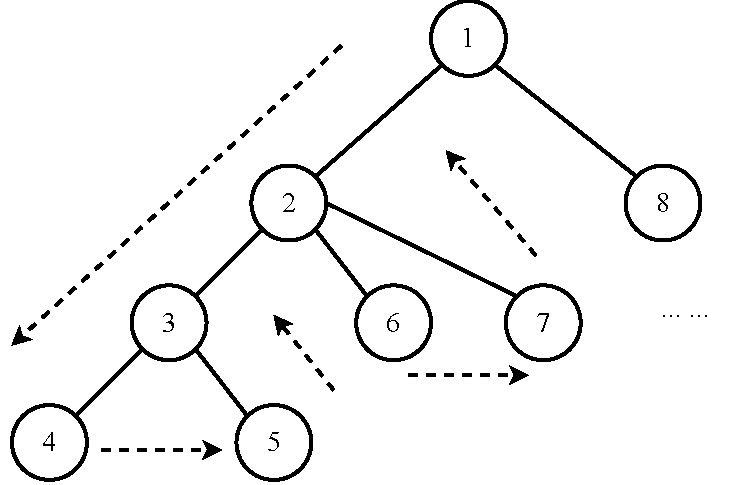
\includegraphics[scale=0.2]{img/dfs-tree-order}
 \caption{深度优先搜索的顺序}
 \label{fig:dfs-tree}
\end{figure}

这样的搜索策略称为深度优先搜索。现实中我们在不经意间广泛使用它。某些编程环境,例如Prolog,使用深度优先作为默认的求值模型。例如一个迷宫可以被一组规则描述:

\lstset{language=Prolog}
\begin{lstlisting}
c(a, b). c(a, e).
c(b, c). c(b, f).
c(e, d), c(e, f).
c(f, c).
c(g, d). c(g, h).
c(h, f).
\end{lstlisting}

其中,断言$c(X, Y)$表示位置$X$和$Y$连通。这一断言是有方向性的。如果要让$Y$和$X$连通,我们可以增加一条对称的断言,或者建立一条无方向性的断言。\cref{fig:directed-graph}给出了一个有向图。任给位置$X$和$Y$,Prolog可以通过下面的程序判定它们之间是否有通路。

\begin{figure}[htbp]
 \centering
 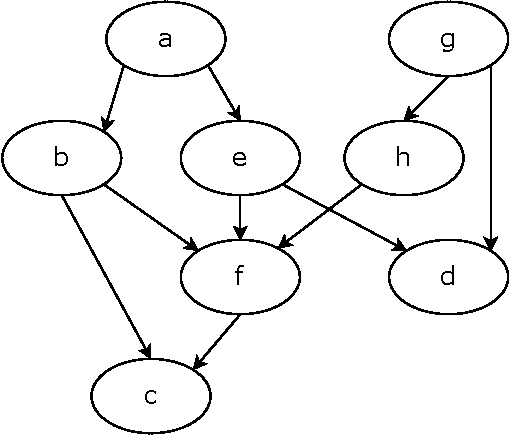
\includegraphics[scale=0.5]{img/directed-graph}
 \caption{一个有向图}
 \label{fig:directed-graph}
\end{figure}

\lstset{language=Prolog}
\begin{lstlisting}
go(X, X).
go(X, Y) :- c(X, Z), go(Z, Y)
\end{lstlisting}

这一程序说:一个位置$X$和自己相通。任意两个不同位置$X$、$Y$,若$X$和$Z$相连,且$Z$和$Y$之间有通路,则$X$和$Y$之间存在通路。显然,$Z$的选择可能不唯一。Prolog选择一个,然后继续搜索。只有当递归搜索失败时才会尝试其它选择。回溯并更换到下一个选项上。这恰好就是深度优先的搜索策略。当只需要找到解,而并不关心步数时,深度优先搜索是很有效的方法。例如,走迷宫中找出的第一个解并不一定是最短路径。

\begin{Exercise}\label{ex:leap-frog}
\Question{修改跳跃青蛙问题的函数式解法,使得它可以解决每侧$n$只青蛙的情况。}
\end{Exercise}

\begin{Answer}[ref = {ex:leap-frog}]
\Question{修改跳跃青蛙问题的函数式解法,使得它可以解决每侧$n$只青蛙的情况。

我们只要利用$n$产生起始、结束状态即可:
\begin{Haskell}
solve n = dfs [[start]] [] where
    dfs [] s = s
    dfs (c:cs) s
        | head c == end = dfs cs (reverse c:s)
        | otherwise = dfs ((map (:c) $ moves $ head c) ++ cs) s
    start = replicate n (-1) ++ [0] ++ replicate n 1
    end = reverse start
\end{Haskell}
}
\end{Answer}

\subsubsection{狼、羊、白菜过河问题}
\index{狼、羊、白菜趣题}

这是一道传统趣题。农夫带着一只狼、一只羊、一筐白菜过河。有一条小船,只有农夫会划船。小船只能装下农夫和另外一样东西。农夫每次只能在狼、羊、白菜中任选一样和他一起过河。但是如果农夫不在,狼会吃掉羊,而羊会吃掉白菜。如何用最快的方法让所有东西都渡过河?

%% \begin{figure}[htbp]
%%  \centering
%%  \includegraphics[scale=0.3]{img/wgc-puzzle}
%%  \caption{狼、羊、白菜过河问题}
%%  \label{fig:wgc-puzzle}
%% \end{figure}

由于狼不会吃掉白菜,农夫可以安全地将羊运到河对岸并返回。接下来无论将狼或白菜中的任何一样运过河,他必须将某一样运回以避免有东西被吃掉。为了寻找最快的渡河方法,我们并发检查所有的选项,比较哪个更快。不考虑渡河的方向,每渡过一次算做一步,往返算两步。我们检查渡河一次后的所有可能、两次后所有可能、三次后的所有可能……直到某次后,所有的东西都到达了对岸结束。并且这一渡河方法在所有可能中胜出,是最快的解法。

如何“并发”检查所有可能的解法?考虑一个抽奖游戏。参与者闭着眼睛从箱子里摸出一个球。箱子里只有一个黑球,其余的球都是白色的。摸到黑球获胜,摸到白球则放回箱子,然后等待下次摸球。为了使游戏公平,可以制定这样一个规则:必须等所有人都摸过之后才能再摸第二次。参与游戏的人站成一队。每次站在队伍前面的人摸球,如果他没有摸到黑球获胜,就站到队尾等待下次摸球。这一队列可以保证游戏的公平。

\begin{figure}[htbp]
 \centering
 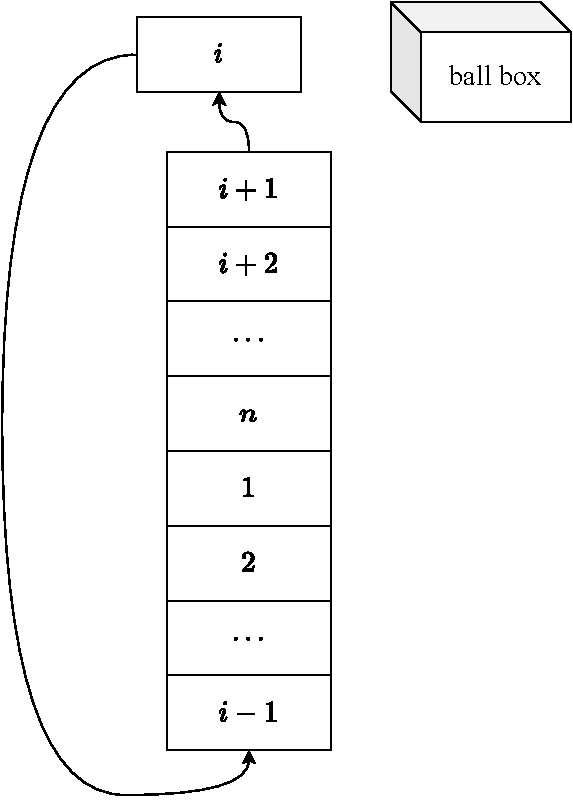
\includegraphics[scale=0.2]{img/luckydraw-queue}
 \caption{第$i$个人出队摸球。如果没有摸到黑球就站到队尾}
 \label{fig:luck-draw}
\end{figure}

用类似的思路来解决渡河问题。用集合$A$、$B$代表河两岸。开始时,集合$A = \{w, g, c, p\}$包含狼、羊、白菜、农夫,集合$B = \nil$。每次将农夫和另外一个元素在集合间移动。如果集合中不存在农夫,则不能含相互冲突的东西。目标是用最少的次数交换$A$、$B$的内容。使用一个队列$Q$包含起始状态$A = \{w, g, c, p\}$、$B=\nil$。只要队列不空,我们就取出头部元素,扩展所有可能的选择。然后将扩展后的状态放回队尾。如果队列头部等于$A=\nil$、$B=\{w, g, c, p\}$,我们就找到了解。\cref{fig:bfs-tree}描述了搜索顺序。同一深度上的所有可能都被检查了,无需进行回溯。

\begin{figure}[htbp]
 \centering
 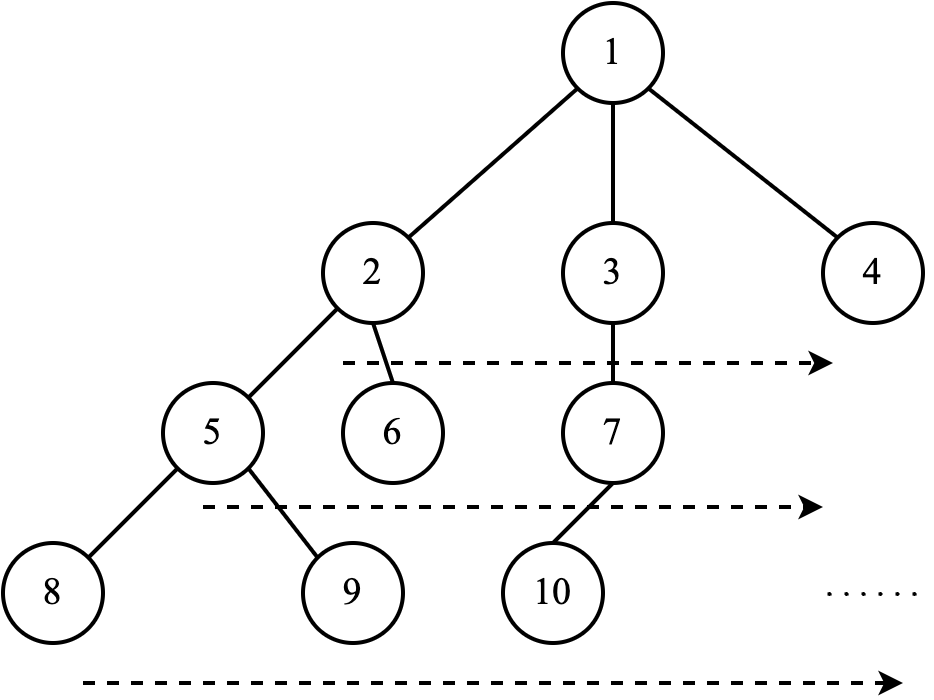
\includegraphics[scale=0.2]{img/bfs-tree-order}
 \caption{从第一个状态开始,检查第二步的所有选项2、3、4;然后检查第3层上的所有选项……}
 \label{fig:bfs-tree}
\end{figure}

可以用4位二进制数来表示集合,每一位表示一种事物,狼$w=1$、羊$g=2$、白菜$c=4$、农夫$p=8$。0表示空集,15表示包含所有事物的集合。值3表示只有狼和羊,此时狼会吃掉羊。同样,值6表示另一种冲突情况。每次我们将最高位(8)和另外一位(4、2、1)从一个数字移动到另一个数字上。可行的移动方法为:

\be
mv\ A\ B = \begin{cases}
  B < 8: & [(A - 8 - i, B + 8 + i) | i \gets [0, 1, 2, 4], i = 0 \text{或} A \overline{\land} i \neq 0]\\
  \text{否则}: & [(A + 8 + i, B - 8 - i) | i \gets [0, 1, 2, 4], i = 0 \text{或} B \overline{\land} i \neq 0]
  \end{cases}
\ee

其中$\overline{\land}$表示按位与运算。我们用队列$Q = \{[(15, 0)]\}$启动搜索:$solve\ Q$。

\be
\begin{array}{rcl}
solve\ \nil & = & \nil \\
solve\ Q & = & \begin{cases}
  A = 0: & reverse\ c, \text{其中} (A, B) = c, (c, Q') = pop\ Q \\
  \text{否则}: & solve\ (pushAll\ (map\ (:c)\ (filter\ (valid\ c)\ (mv\ A\ B)))\ Q')
  \end{cases}
\end{array}
\ee

其中函数$valid\ c$检查新的移动结果$(A, B)$是存在冲突。不能是3、6,并且尚未尝试过,不存在于$c$中:

\be
A, B \neq 3 \text{或} 6, (A, B) \notin c
\ee

下面是对应的迭代实现:

\begin{algorithmic}[1]
\Function{Solve}{}
  \State $S \gets []$
  \State $Q \gets \{[(15, 0)]\}$
  \While{$Q \neq \nil$}
    \State $C \gets $ \Call{DeQ}{$Q$}
    \If{$C[1] = (0, 15)$}
      \State \textproc{Add}($S$, \Call{Reverse}{$C$})
    \Else
      \For{each $m$ in \Call{Moves}{$C$}}
        \If{\Call{Valid}{$m, C$}}
          \State \Call{EnQ}{$Q, m \cons C$}
        \EndIf
      \EndFor
    \EndIf
  \EndWhile
  \State \Return $S$
\EndFunction
\end{algorithmic}

下面列出了两个最优解。

\btab{l|c|l}
左 & 河 & 右 \\
\hline
狼、羊、白菜、农夫 &   & \\
狼、白菜 &   & 羊、农夫 \\
狼、白菜、农夫 &   & 羊 \\
白菜 &   & 狼、羊、农夫 \\
羊、百次、农夫 &   & 狼 \\
羊 &   & 狼、白菜、农夫 \\
羊、农夫 &   & 狼、白菜 \\
 &  & 狼、羊、白菜、农夫
\etab

\btab{l|c|l}
左 & 河 & 右 \\
\hline
狼、羊、白菜、农夫 & & \\
狼、白菜 & & 羊、农夫 \\
狼、白菜、农夫 & & 羊 \\
狼 & & 羊、白菜、农夫 \\
狼、羊、农夫 & & 白菜 \\
羊 & & 狼、白菜、农夫 \\
羊、农夫 & & 狼、白菜 \\
 & & 狼、羊、白菜、农夫
\etab

\subsubsection{倒水问题}
\index{倒水问题}

有两个水瓶,一个9升、一个4升。如何才能从河中取出6升水?这个题目可以追溯到古希腊。有一个故事说法国数学家泊松在孩童时代就解决了这个问题。在好莱坞电影《虎胆龙威3》中也出现了这个问题。数学家波利亚在《如何解题》中用倒推法给出了一个解\cite{how-to-solve-it}。最终状态大瓶子中盛有6升水。倒数第二步时,从9升的瓶子中倒出3升水。为了达成这一点,小瓶子中需要盛有1升水。如\cref{fig:jugs-r1}所示。

%% \begin{figure}[htbp]
%%  \centering
%%  \includegraphics[scale=0.5]{img/jugs-start}
%%  \caption{9升、4升的瓶子}
%%  \label{fig:jugs-start}
%% \end{figure}

\begin{figure}[htbp]
 \centering
 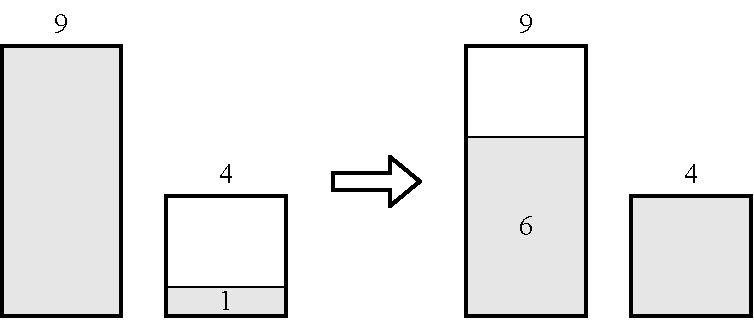
\includegraphics[scale=0.2]{img/jugs-last}
 \caption{最后两步}
 \label{fig:jugs-r1}
\end{figure}

只要倒满9升的瓶子,然后连续两次倒入4升的瓶子,并将4升的瓶子倒空,就可以得到1升水。如\cref{fig:jugs-r2}所示。倒推法是一种策略,而不是具体的算法。它无法回答如何从899升和1147升的瓶子得到2升水。

\begin{figure}[htbp]
 \centering
 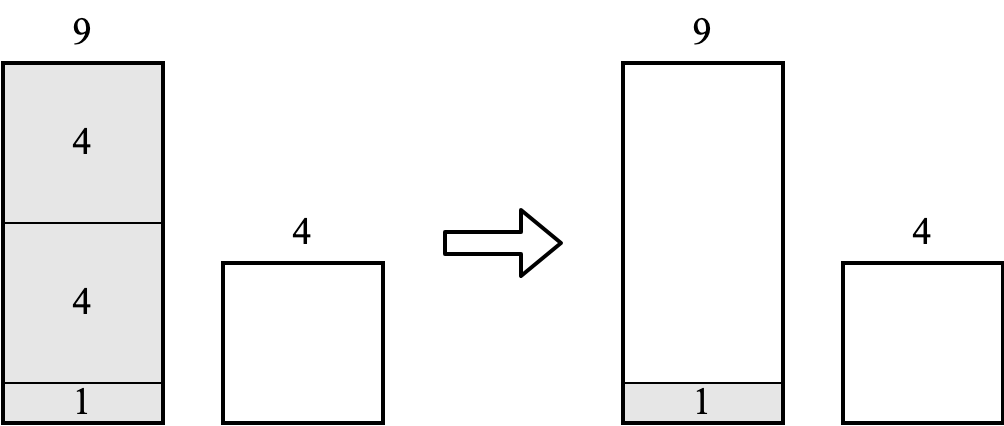
\includegraphics[scale=0.2]{img/jugs-last-two}
 \caption{将大瓶倒满,然后倒入小瓶两次}
 \label{fig:jugs-r2}
\end{figure}

大小两个瓶子$B, A$,每次有6种操作:(1) 小瓶子$A$装满水;(2) $B$装满水;(3) 倒空$A$;(4) 倒空$B$;(5) 将$A$中的水倒入$B$;(6) 将$B$倒入$A$。下表是一系列倒水动作,假设容积$a < b < 2a$。

\btab{l|l|l}
$A$ & $B$ & 操作 \\
\hline
0 & 0 & 开始 \\
a & 0 & 倒满$A$ \\
0 & a & 将$A$倒入$B$ \\
a & a & 倒满$A$ \\
2a - b & b & 将$A$倒入$B$ \\
2a - b & 0 & 倒光$B$ \\
0 & 2a - b & 将$A$倒入$B$ \\
a & 2a - b & 倒满$A$ \\
3a - 2b & b & 将$A$倒入$B$ \\
... & ... & ... \\
\etab

无论何种操作,每个瓶中水的容量总可以表示为$xa + yb$的形式,其中$a$、$b$是容量,$x$、$y$是整数。根据数论中的结论,我们可以判断是否能得到$g$升水:当且仅当$g$能够被$a$、$b$的最大公约数整除时。即:$gcd(a, b) | g$。如果$gcd(a, b) = 1$($a$、$b$互素),可以得到任意自然数$g$升水。虽然可以判定是否有解,但我们并不知道具体的倒水步骤。解出丢番图方程$g = xa + yb$中的$x$、$y$,可以得到一组操作。设$x > 0, y < 0$,我们倒满瓶$A$共$x$次、倒空瓶$B$共$y$次。例如小瓶容积$a=3$、大瓶容积$b=5$,要取得$g=4$升水。因为$4 = 3 \times 3 - 5$,可以设计下列步骤:

\btab{l|l|l}
$A$ & $B$ & 操作 \\
\hline
0 & 0 & 开始 \\
3 & 0 & 倒满$A$ \\
0 & 3 & 将$A$倒入$B$ \\
3 & 3 & 倒满$A$ \\
1 & 5 & 将$A$倒入$B$ \\
1 & 0 & 将$B$倒空 \\
0 & 1 & 将$A$倒入$B$ \\
3 & 1 & 倒满$A$ \\
0 & 4 & 将$A$倒入$B$ \\
\etab

共倒满$A$瓶3次、倒空$B$瓶1次。我们可以利用数论中\textbf{扩展欧几里得算法}找出整数解$x$和$y$:

\be
(d, x, y) = gcd_{ext}(a, b)
\ee

其中$d = gcd(a, b)$,$ax + by = d$。设$a < b$,商$q$和余数$r$,满足关系$b = a q + r$。公约数$d$整除$a$、$b$,因此$d$也整除$r$。由于$r < a$,可以通过寻找$a$和$r$的最大公约数减小问题的规模。

\be
(d, x', y') = gcd_{ext}(r, a)
\label{eq:recursive-ext-gcd}
\ee

其中$d = x' r + y' a$。将$r = b - a q$代入:

\be
\begin{array}{rcl}
d & = & x' (b - a q) + y' a \\
  & = & (y' - x' q) a + x' b
\end{array}
\ee

与$d = ax + by$对比,有下面递归关系:

\be
\begin{cases}
  x & = y' - x' \dfrac{b}{a} \\
  y & = x'
\end{cases}
\ee

递归的边界条件发生在$a=0$时:$gcd(0, b) = b = 0 a + 1 b$。这样扩展欧几里得算法定义为:

\be
\begin{array}{rcl}
gcd_{ext}(0, b) & = & (b, 0, 1) \\
gcd_{ext}(a, b) & = & (d, y' - x' \dfrac{b}{a}, x')
\end{array}
\ee

其中$d$、$x'$、$y'$的定义如\cref{eq:recursive-ext-gcd}。如果$g = md$,则$mx$和$my$就是倒水问题的一个解;如果$x < 0$,例如$gcd_{ext}(4, 9) = (1, -2, 1)$。由于$d = x a + y b$,我们不断将$x$加$b$,同时将$y$减$a$,直到$x$大于0。这样得到的解并不一定最优。例如用3升、5升的瓶子,获取4升水,扩展欧几里得算法给出23步:

\begin{Verbatim}[fontsize=\footnotesize]
[(0,0),(3,0),(0,3),(3,3),(1,5),(1,0),(0,1),(3,1),
(0,4),(3,4),(2,5),(2,0),(0,2),(3,2),(0,5),(3,5),
(3,0),(0,3),(3,3),(1,5),(1,0),(0,1),(3,1),(0,4)]
\end{Verbatim}

而最优解只需要6步:

\begin{Verbatim}[fontsize=\footnotesize]
[(0,0),(0,5),(3,2),(0,2),(2,0),(2,5),(3,4)]
\end{Verbatim}

丢番图方程$g = x a + b y$有无穷多个解,$|x| + |y|$越小,所需步骤越少。我们可以采用类似“过河问题”的思路。在6种操作中(倒满$A$、倒满$B$、将$A$倒入$B$……)“并行”尝试出最优解。使用一个队列来安排所有的尝试。队列中的元素是一系列值对$(p, q)$,$p$、$q$分别是两瓶中水的体积,记录了从开始到最后的倒水操作。开始时队列内容为:$\{[(0, 0)]\}$。

\be
solve\ a\ b\ g = bfs \{ [(0, 0)] \}
\ee

只要队列不空,我们从头部取出一操作序列。如果序列中的最后状态包含$g$升水,我们就找到了一个解。我们将序列逆序输出;否则我们扩展最后的状态,尝试6种可能,去掉重复的并入队。

\be
\begin{array}{rcl}
bfs\ \nil & = & [\ ] \\
bfs\ Q & = & \begin{cases}
  p \text{或} q = g: & \textit{reverse}\ s, \text{其中} (p, q) = head\ s, (s, Q') = pop\ Q \\
  \text{否则}: & bfs\ (pushAll\ (map\ (:s)\ (try\ s))\ Q')
    \end{cases}
\end{array}
\ee

\be
try\ s = filter\ (\notin s)\ [f\ (p, q) | f \gets \{fl_A, fl_B, pr_A, pr_B, em_A, em_B\}]
\ee

其中:

\be
\begin{cases}
fl_A\ (p, q) = (a, q) \\
fl_B\ (p, q) = (p, b) \\
em_A\ (p, q) = (0, q) \\
em_B\ (p, q) = (p, 0) \\
pr_A\ (p, q) = (\max(0, p + q - b), \min(x + y, b)) \\
pr_B\ (p, q) = (\min(x + y, a), \max(0, x + y - a)) \\
\end{cases}
\ee

这一方法总返回最快的步骤。我们无需在队列的每个元素中保存操作步骤,可以利用一个全局历史记录,如\cref{fig:water-jugs}。初始状态为(0, 0)。只有fill A和fill B可行。接下来在记录(3, 0)的基础上尝试fill B,记录新结果(3, 5)。在(3, 0)的基础上尝试empty A将回到初始状态(0, 0)。我们跳过这一选项。图中灰色状态是重复的。我们可以给\cref{fig:water-jugs}中的每个节点增加一个父引用,利用它回溯到初始状态。

\begin{figure}[htbp]
  \centering
  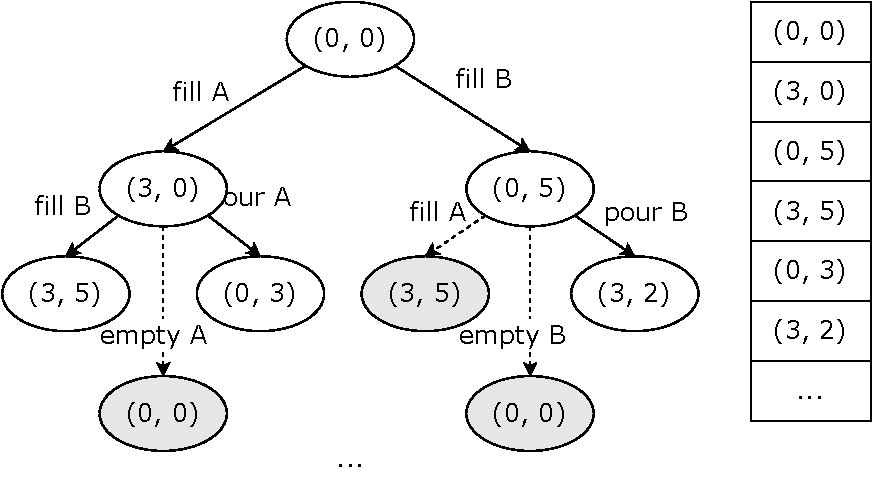
\includegraphics[scale=0.5]{img/water-jugs}
  \caption{全局记录}
  \label{fig:water-jugs}
\end{figure}

\begin{algorithmic}[1]
\Function{Solve}{$a, b, g$}
  \State $Q \gets \{(0, 0, \text{NIL})\}$
  \State $V \gets \{(0, 0, \text{NIL})\}$  \Comment{全局记录集合}
  \While{$Q \neq \nil$}
    \State $s \gets$ \Call{Pop}{$Q$}
    \If{$p(s) = g$ 或 $q(s) = g$}
      \State \Return \Call{Back-track}{$s$}
    \Else
      \For{each $c$ in \Call{Expand}{$s, a, b$}}
        \If{$c \neq s$ 且 $c \notin V$}
          \State \Call{Push}{$Q, c$}
          \State \Call{Add}{$V, c$}
        \EndIf
      \EndFor
    \EndIf
  \EndWhile
  \State \Return NIL
\EndFunction
\Statex
\Function{Expand}{$s, a, b$}
  \State $p \gets p(s), q \gets q(s)$
  \State \Return $[(a, q, s), (p, b, s), (0, q, s), (p, 0, s), (\max(0, p + q - b), \min(p + q, b), s), (\min(p + q, a), \max(0, p + q - a), s)]$
\EndFunction
\Statex
\Function{Back-track}{$s$}
  \State $r \gets [\ ]$
  \While{$s \neq$ NIL}
    \State $(p, q, s') = s$
    \State $r \gets (p, q) \cons r$
    \State $s \gets s'$
  \EndWhile
  \State \Return $r$
\EndFunction
\end{algorithmic}

\begin{Exercise}\label{ex:water-jugs-puzzle}
\Question{改进扩展欧几里得算法,寻找线性组合使得$|x| + |y|$最小,以解决倒水问题。}
\end{Exercise}

\begin{Answer}[ref = {ex:water-jugs-puzzle}]
\Question{改进扩展欧几里得算法,寻找线性组合使得$|x| + |y|$最小,以解决倒水问题。

\begin{Haskell}
import Data.List
import Data.Function (on)

-- Extended Euclidean Algorithm
gcmex a 0 = (a, 1, 0)
gcmex a b = (g, y', x' - y' * (a `div` b)) where
  (g, x', y') = gcmex b (a `mod` b)

-- Solve the linear Diophantine equation ax + by = c
solve a b c | c `mod` g /= 0 = (0, 0, 0, 0) -- no solution
            | otherwise = (x1, u, y1, v)
  where
    (g, x0, y0) = gcmex a b
    (x1, y1) = (x0 * c `div` g, y0 * c `div` g)
    (u, v) = (b `div` g, a `div` g)

-- Minimize |x| + |y|
jars a b c = (x, y) where
  (x1, u, y1, v) = solve a b c
  x = x1 - k * u
  y = y1 + k * v
  k = minimumBy (compare `on` (\i -> abs (x1 - i * u) +
                                     abs (y1 + i * v))) [-m..m]
  m = max (abs x1 `div` u) (abs y1 `div` v)

-- Populate the steps
water a b c = if x > 0 then pour a x b y
              else map swap $ pour b y a x
  where
    (x, y) = jars a b c

-- Pour from a to b, fill a for x times, and empty b for y times.
pour a x b y = steps x y [(0, 0)]
  where
    steps 0 0 ps = reverse ps
    steps x y ps@((a', b'):_)
      | a' == 0 = steps (x - 1) y ((a, b'):ps)  -- fill a
      | b' == b = steps x (y + 1) ((a', 0):ps)  -- empty b
      | otherwise = steps x y ((max (a' + b' - b) 0,
                                min (a' + b') b):ps) -- a to b
\end{Haskell}

更多内容,请参见《同构——编程中的数学》第二章,2.2.3节。
}
\end{Answer}

\subsubsection{华容道}
\index{华容道}

传统玩具华容道是滑块类游戏,如\cref{fig:klotski-cn}。国外称Klotski。滑块大小、布局会有不同。华容道有10个滑块,上面标有数字或者图案。最小的滑块大小为一个单位的正方形,最大的一块为$2 \times 2$单位。在棋盘下方的中间,有一个宽度为2个单位长的缺口。最大的一块代表曹操,其他的为刘备手下的五虎上将和士兵。游戏的目标是要通过滑动,将曹操移动到棋盘最下方逃走。\cref{fig:klotski-jp}是日本游戏“箱子中的女儿”,最大的一块代表女儿,剩余滑块代表其他家庭成员。

\begin{figure}[htbp]
 \centering
 \subcaptionbox{起始布局}{\includegraphics[scale=0.5]{img/klotski-cn1}} \hspace{.01\textwidth}
 \subcaptionbox{移动若干步后的样子}{\includegraphics[scale=0.5]{img/klotski-cn2}}
 \caption{华容道游戏}
 \label{fig:klotski-cn}
\end{figure}

\begin{figure}[htbp]
 \centering
 \includegraphics[scale=0.5]{img/klotski-jp}
 \caption{日本的“箱子中的女儿”游戏}
 \label{fig:klotski-jp}
\end{figure}

我们用$5 \times 4$矩阵来代表棋盘,行列从0开始。1到10个数字代表棋子。0代表空位置。矩阵$M$给出了华容道的初始状态。值为$i$的格子表示有棋子占据。布局用字典$L$代表。$L[i]$棋子$i$覆盖的位置集合。例如$L[4] = \{(2, 1), (2, 2)\}$表示第4个棋子覆盖了位置$(2, 1)$、$(2, 2)$。我们可以把棋盘上的20个位置编号为0到19,把行列转化为编号:$c = 4y + x$。这样第四个棋子占据$L[4] = \{9, 10\}$。

\[
\begin{array}{cc}
M = \left [
  \begin{array}{cccc}
  1 & 10 & 10 & 2 \\
  1 & 10 & 10 & 2 \\
  3 & 4 & 4 & 5 \\
  3 & 7 & 8 & 5 \\
  6 & 0 & 0 & 9
  \end{array}
\right ] &
L = \left \{
  \begin{array}{l}
  1 \mapsto \{0, 4\}, 2 \mapsto \{3, 7\}, 3 \mapsto \{8, 12\}, \\
  4 \mapsto \{9, 10\}, 5 \mapsto \{11, 15\}, \\
  6 \mapsto \{16\}, 7 \mapsto \{ 13 \}, 8 \mapsto \{ 14 \}, \\
  9 \mapsto \{ 19 \}, 10 \mapsto \{1, 2, 5, 6\}
  \end{array}
\right \}
\end{array}
\]

我们可以定义映射$\varphi(M) \mapsto L$和逆映射$\varphi^{-1}(L) \mapsto M$在棋盘和布局间转换:

\begin{algorithmic}[1]
\Function{$\varphi$}{$M$}
  \State $L \gets \{ \}$
  \For{$y \gets 0 \sim 4$}
    \For{$x \gets 0 \sim 3$}
      \State $k \gets M[y][x]$
      \State $L[k] \gets$ \Call{Add}{$L[k], 4y + x$}
    \EndFor
  \EndFor
  \State \Return $L$
\EndFunction
\Statex
\Function{$\varphi^{-1}$}{$L$}
  \State $M \gets [[0] \times 4] \times 5$
  \For{each $(k \mapsto S)$ in $L$}
    \For{each $c$ in $S$}
      \State $x \gets c \bmod 4, y \gets \lfloor c / 4\rfloor$
      \State $M[y][x] \gets k$
    \EndFor
  \EndFor
  \State \Return $M$
\EndFunction
\end{algorithmic}

我们检查全部10个棋子,看看能否在上下左右4个方向移动1格。在矩阵棋盘上,移动表示为$(\Delta y, \Delta x) = (0, \pm 1), (\pm 1, 0)$,在布局上,四个方向分别表示为位移$d = \pm 1, \pm 4$,例如棋子$L[i] = \{c_1, c_2\}$向左移动变为$\{c_1 -1, c_2 -1\}$。这里要排除两个特殊情况:$d = 1, c \bmod 4 = 3$和$d = -1, c \bmod 4 = 0$,防止棋子从一侧边界跳到另一侧。考虑两个空位四周最多有8种移动可能。例如第一步只有4种可能:第6块向右;第7或第8块向下;第9块向左。\cref{fig:klotski-valid-move}描述列如何检查移动可行。

\begin{figure}[htbp]
 \centering
 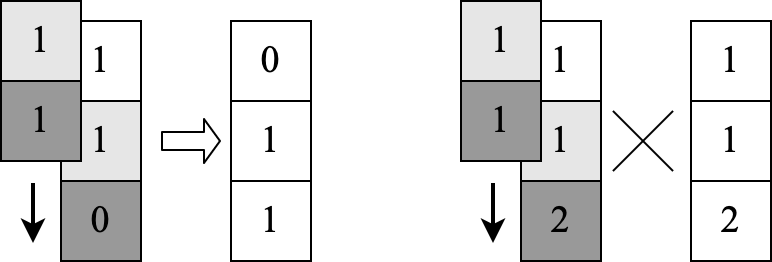
\includegraphics[scale=0.3]{img/klotski-valid-mv}
 \caption{左侧:两个标1的格子都可移动;右侧:下方标1的格子和标2的格子冲突。}
 \label{fig:klotski-valid-move}
\end{figure}

为了确定可否移动,我们检查棋子$k$移动到的目标格子,如果为0或者$k$则可移动:

\be
\begin{array}{rl}
valid\ L[k]\ d: & \\
\forall c \in L[k] \Rightarrow & y = \lfloor c / 4 \rfloor + \lfloor d / 4 \rfloor, x = (c \bmod 4) + (d \bmod 4), \\
& (0, 0) \leq (y, x) \leq (4, 3), M[y][x] \in \{k, 0\}
\end{array}
\ee

经过一系列移动可能回到某个布局。仅避免棋盘矩阵相同是不够的,虽然下面的$M_1 \neq M_2$,但它们本质上是相同的布局。

\[
\begin{array}{cc}
M_1 = \left [
  \begin{array}{cccc}
  1 & 10 & 10 & 2 \\
  1 & 10 & 10 & 2 \\
  3 & 4 & 4 & 5 \\
  3 & 7 & 8 & 5 \\
  6 & 0 & 0 & 9
  \end{array}
\right ] &
M_2 = \left [
  \begin{array}{cccc}
  2 & 10 & 10 & 1 \\
  2 & 10 & 10 & 1 \\
  3 & 4 & 4 & 5 \\
  3 & 7 & 6 & 5 \\
  8 & 0 & 0 & 9
  \end{array}
\right ]
\end{array}
\]

我们需要比较布局来避免重复。忽略具体棋子,定义归一化布局为集合:$\|L\| = \{ p | (k \mapsto p) \in L\}$,也就是字典$L$中所有值的集合。上面两个矩阵的归一化布局都等于\{\{1, 2, 5, 6\}, \{0, 4\}, \{3, 7\}, \{8, 12\}, \{9, 10\}, \{11, 15\}, \{16\}, \{13\}, \{14\}, \{19\}\}。左右对称的布局也是一种重复,需要避免。例如下面的$M_1$和$M_2$对称。

\[
\begin{array}{cc}
M_1 = \left [
  \begin{array}{cccc}
  10 & 10 & 1 & 2 \\
  10 & 10 & 1 & 2 \\
  3 & 5 & 4 & 4 \\
  3 & 5 & 8 & 9 \\
  6 & 7 & 0 & 0
  \end{array}
\right ] &
M_2 = \left [
  \begin{array}{cccc}
  3 & 1 & 10 & 10 \\
  3 & 1 & 10 & 10 \\
  4 & 4 & 2 & 5 \\
  7 & 6 & 2 & 5 \\
  0 & 0 & 9 & 8
  \end{array}
\right ]
\end{array}
\]

它们的归一化布局也是对称的。我们定义归一化布局的对称变换:

\be
mirror(\|L\|) = \{\{ f(c) | c \in s \} | s \in \|L\|\}
\ee

其中$f(c) = 4y' + x', y' = \lfloor c / 4 \rfloor, x' = 3 - (c \bmod 4)$。我们使用一个队列进行搜索,队列中每个元素包含两部分:一系列移动和这些移动导致的布局。每次移动为$(k, d)$,表示在棋盘上移动棋子$k$,方向为$d$(值为$\pm 1, \pm 4$)。队列初始化为$Q = \{(s, [\ ])\}$,其中$s$是起始布局。只要$Q \neq \nil$,我们就从头部取出一个元素,检查最大的棋子(编号10)是否到达目标位置$t = \{13, 14, 17, 18\}$,即$L[10] = t$。如到达则结束;否则,我们尝试上下左右移动每块棋子,把所有可行的、不重复布的局移动方案$(k, d)$入队。在搜索过程中,我们用集合$H$记录归一化布局以避免重复。

\be
\begin{array}{rcl}
solve\ \nil\ H\ & = & [\ ] \\
solve\ Q\ H\ & = & \begin{cases}
  L[10] = t: & \textit{reverse}\ ms, \text{其中} ((L, ms), Q') = pop\ Q \\
  \text{否则}: & solve\ (pushAll\ cs\ Q')\ H' \\
  \end{cases}
\end{array}
\ee

其中$cs = [(move\ L\ e, e \cons ms) | e \gets expand\ L]$是新产生的移动方案。

\be
\begin{array}{rl}
expand\ L = \{(k, d) | & k \gets [1, 2, ..., 10], d \gets [\pm 1, \pm 4], \\
  &  valid\ k\ d, unique\ k\ d \} \\
\end{array}
\ee

$move$把棋子$L[k]$移动$d$成为:$move\ L\ (k, d) = map\ (+ d)\ L[k]$。$unique$判断新归一化布局$\|L'\| \notin H$,镜像$mirror(\|L'\|) \notin H$不在历史记录中。如果没有重复,更新它们到新记录$H'$用于后继搜索。下面是对应的迭代式实现。“横刀立马”布局的最少步数解共116步(每步移动1格),最后3步如下:

\begin{algorithmic}[1]
\Function{Solve}{$s, e$}
  \State $H \gets \{\|s\|\}$
  \State $Q \gets \{(s, \nil)\}$
  \While{$Q \neq \nil$}
    \State $(L, p) \gets$ \Call{Pop}{$Q$}
    \If{$L[10] = e$}
      \State \Return $(L, p)$
    \Else
      \For{each $L'$ in \Call{Expand}{$L, H$}}
        \State \Call{Push}{$Q, (L', L)$}
        \State \Call{Add}{$H, \|L'\|$}
      \EndFor
    \EndIf
  \EndWhile
  \State \Return $\nil$
\EndFunction
\end{algorithmic}

\begin{Verbatim}[fontsize=\footnotesize]
['5', '3', '2', '1']
['5', '3', '2', '1']
['7', '9', '4', '4']
['A', 'A', '6', '0']
['A', 'A', '0', '8']

['5', '3', '2', '1']
['5', '3', '2', '1']
['7', '9', '4', '4']
['A', 'A', '0', '6']
['A', 'A', '0', '8']

['5', '3', '2', '1']
['5', '3', '2', '1']
['7', '9', '4', '4']
['0', 'A', 'A', '6']
['0', 'A', 'A', '8']
\end{Verbatim}

\index{BFS} \index{广度优先搜索}
过河问题、倒水问题、华容道游戏的解法有共同的结构。和深度优先类似,它们都有起始、终止状态。在过河问题中,起始状态是农夫、狼、羊、白菜在河的一岸,对岸为空;终止状态是全部渡河到了对岸。倒水问题的起始状态是两个空瓶子,而终止状态是某个瓶子盛有指定容量的水。华容道问题的起始状态是某种布局(“横刀立马”),终止状态是另外一个布局,其中最大的棋子移动到了指定的位置。每个问题都有相应的规则,可以从一个状态转移到另外一个状态。我们“并行”尝试可能选项。在同一步内的选项未尝试完之前,我们不会进一步深入搜索。这就保证了最小步骤解在其它解之前出现。由于向水平方向扩展,这种方法称为广度优先搜索。\cref{fig:dfs-bfs-tree}给出了广度、深度优先搜索的对比。

\begin{figure}[htbp]
 \centering
 \subcaptionbox{深度优先搜索}{ 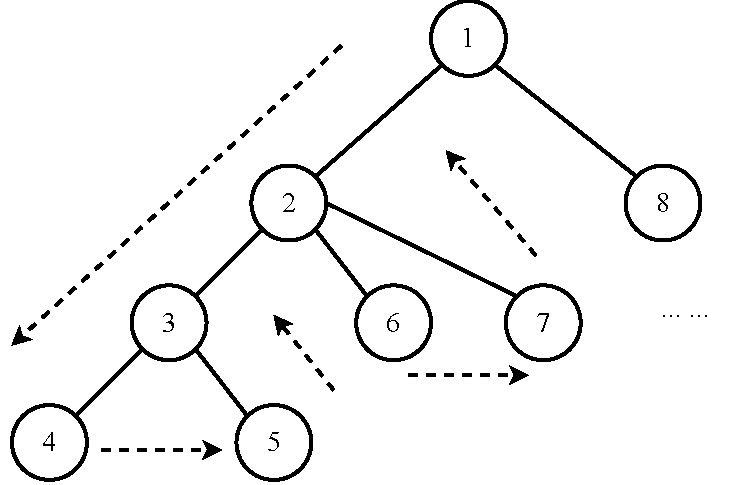
\includegraphics[scale=0.15]{img/dfs-tree-order}}
 \subcaptionbox{广度优先搜索}{ \includegraphics[scale=0.15]{img/bfs-tree-order}}
 \caption{深度和广度优先搜索的顺序}
 \label{fig:dfs-bfs-tree}
\end{figure}

由于我们无法真正的“并行”搜索,广度优先搜索使用队列来记录尝试。从队列头部不断取出步骤较少的候选项,从队列尾部不断加入步骤较多的新候选项。广度优先搜索提供了一种简单的方法寻找最少步骤解,但它不能直接搜索其它最优解。考虑如\cref{fig:weighted-dag}的有向图,每段路径长度不同,我们无法用广度优先搜索找出两个城市之间的最短路径。注意从城市$a$到城市$c$之间的最短路径并非经过最少城市的$a \to b \to c$。这条路径的总长度为22;而是经过更多城市的路径$a \to e \to f \to c$,他的总长度只有20。

\begin{figure}[htbp]
 \centering
 \includegraphics[scale=0.5]{img/weighted-dag}
 \caption{带权重的有向图}
 \label{fig:weighted-dag}
\end{figure}

\begin{Exercise}\label{ex:conway-slide-puzzle}
\Question{康威\footnote{约翰$\cdot$康威(1937-2020),英国数学家。}提出了一种滑动趣题。\cref{fig:conway7}给出的是一种简化的版本。8个圆圈中的7个已经放入了棋子,每个棋子上标有编号1到7。如果和棋子相邻的圆圈是空的,则棋子可以滑动过去。圆圈间如果有连线,则表示它们是相连的。目标是将棋子从顺序1、2、3、4、5、6、7通过滑动反转成7、6、5、4、3、2、1。编写一个程序解决康威滑动问题。
\begin{center}
 \centering
 %\input{img/conway7.tex}
 \includegraphics[scale=0.5]{img/conway-7-slide}
 \captionof{figure}{康威滑动趣题}
 \label{fig:conway7}
\end{center}
}
\end{Exercise}

\begin{Answer}[ref = {ex:conway-slide-puzzle}]
\Question{康威滑动趣题。

我们用0到7这8个数字的排列代表棋子的分步,其中0代表空位。空位前、后的棋子可以滑入空位。我们将其表示为0在排列中左右移动。向右移动到尾部时,继续向右则回到头部,向左到头部时,继续向左回到尾部。特别地,如果空位0在排列头部,它可以和第5位置上的棋子交换,反之亦可。康威滑动游戏的解很长,需要12948步移动才能反转棋子。人类玩家会失去耐心。其中最后几步如下:

\begin{Haskell}
start = [0..7]
end = 0:[7,6..1]

solve1 = dfs [[start]] where
  dfs [] = []
  dfs (c:cs)
    | head c == end = reverse c
    | otherwise = dfs ((map (:c) $ moves c) ++ cs)

moves (s:visited) = filter (`notElem` visited) [fwd s, bk s, cut s]
  where
    fwd xs = case break (0 ==) xs of
      (as, 0:b:bs) -> as ++ (b:0:bs)
      (a:as, [0]) -> 0:as ++ [a]
    bk xs = case break (0 ==) xs of
      ([], 0:bs) -> bs ++ [0]
      (as, 0:bs) -> (init as) ++ (0 : last as : bs)
    cut xs = case splitAt 4 xs of
      ((0:as), (x:bs)) -> (x:as) ++ (0:bs)
      ((x:as), (0:bs)) -> (0:as) ++ (x:bs)
      _ -> xs
\end{Haskell}

\begin{Verbatim}[fontsize=\footnotesize]
...
[1,0,7,6,5,4,3,2],[1,7,0,6,5,4,3,2],[1,7,6,0,5,4,3,2],[1,7,6,5,0,4,3,2],
[1,7,6,5,4,0,3,2],[1,7,6,5,4,3,0,2],[1,7,6,5,4,3,2,0],[0,7,6,5,4,3,2,1]
\end{Verbatim}
}
\end{Answer}


\subsection{贪心算法}
\index{贪心算法}

人们需要“最好”的解来节省时间、空间、成本、能量。使用有限的资源搜索最优解并不容易。有很多问题不存在多项式时间的解法。仅对一些特定问题存在简单方法找到最优解。

\subsubsection{哈夫曼编码} \index{哈夫曼编码}
哈夫曼编码是一种用最小长度对信息编码的方法。早期的ASCII码使用7位二进制数对字母、数字、符号编码,可以表达$2^7 = 128$个字符。只用0、1,我们至少需要$\log_2 n$位分辨$n$个不同字符。下面是大写英文字母的码表,将字母A到Z映射为0到25。每个编码5位。零被扩充到5位00000而非0。这样的编码方式称为定长编码。

\btab{l|l||l|l}
字符 & 编码 & 字符 & 编码 \\
\hline
A & 00000 & N & 01101 \\
B & 00001 & O & 01110 \\
C & 00010 & P & 01111 \\
D & 00011 & Q & 10000 \\
E & 00100 & R & 10001 \\
F & 00101 & S & 10010 \\
G & 00110 & T & 10011 \\
H & 00111 & U & 10100 \\
I & 01000 & V & 10101 \\
J & 01001 & W & 10110 \\
K & 01010 & X & 10111 \\
L & 01011 & Y & 11000 \\
M & 01100 & Z & 11001 \\
\hline
\etab

文本“INTERNATIONAL”可以编码为65位的二进制数:

\begin{Verbatim}[fontsize=\footnotesize]
00010101101100100100100011011000000110010001001110101100000011010
\end{Verbatim}

另一种方式是变长编码。用一位二进制数0代表A,用两位二进制数10代表C,用5位二进制数11001代表Z。虽然可以显著缩短编码长度。但在解码时会造成歧义。例如二进制数1101,我们不知道它是1,后面跟着101(表示“BF”),还是110,后面跟着1(表示“GB”),或是1101(表示N)。摩尔斯电码是变长编码。最常用的字符E编码为“.”,字符Z编码为“- -..”。使用特殊终止符分割编码,所以不会发生歧义。下面是一个特殊的无歧义码表:

\btab{l|l||l|l}
字符 & 编码 & 字符 & 编码 \\
\hline
A & 110 & E & 1110 \\
I & 101 & L & 1111 \\
N & 01 & O & 000 \\
R & 001 & T & 100 \\
\hline
\etab

文本“INTERNATIONAL”编码为38位的二进制数:

\begin{Verbatim}[fontsize=\footnotesize]
10101100111000101110100101000011101111
\end{Verbatim}

按上表解码不会遇到有歧义的字符。这是因为没有任何编码是其它编码的前缀。这样的编码称为\textbf{前缀码}\footnote{英文叫做prefix-code,而不是无前缀码.}。前缀码不需要分隔符,编码长度可进一步缩短。这自然引发了一个问题:给定文本,能否找到码表使得编码长度最短?1951年,麻省理工学院的学生大卫$\cdot$哈夫曼\cite{Huffman}的老师罗伯特$\cdot$费诺在课上宣布:谁解出了这个问题就不用参加期末考试了。哈夫曼尝试了很久。他几乎放弃了,开始准备考试。恰在此时,他灵光乍现找到了解法。哈夫曼根据文本中字符出现的频率构造码表。最“常见”的字符编码最短。首先处理文本获得每个字符出现的次数。定义字符的权重是它出现的次数或概率。哈夫曼用二叉树产生前缀码。字符保存于叶子节点。从根节点遍历产生编码。向左前进时添加0,向右前进时添加1,如\cref{fig:huffman-tr}。例如,从根节点遍历到N的路径是,向左然后向右到达N。因此N编码为01;字符A的路径是:右、右,左,编码是110。

\begin{figure}[htbp]
 \centering
 \includegraphics[scale=0.5]{img/huffman-tr}
 \caption{哈夫曼树}
 \label{fig:huffman-tr}
\end{figure}

这棵树还可以解码。扫描二进制数,0向左、1向右。到达叶子时,节点上的字符就是解码内容。然后重新返回根节点继续扫描。哈夫曼用自底向上的方法构造树。开始时,每个字符都放入一个叶子节点中。每次选出两个权重最小的节点合并成一个分支。分支权重为两个子树的权重和。不断选择权重最小的两棵树合并,最后得到一棵树,如\cref{fig:huffman-build}。

\captionsetup[subfigure]{labelformat=empty, margin=10pt}
\begin{figure}[htbp]
 \centering
 \subcaptionbox{第一步}{ \includegraphics[scale=0.4]{img/huffman-tr1}}
 \subcaptionbox{第二步}{ \includegraphics[scale=0.4]{img/huffman-tr2}}
 \subcaptionbox{第三步}{ \includegraphics[scale=0.4]{img/huffman-tr3}} \\
 \subcaptionbox{第四步}{ \includegraphics[scale=0.4]{img/huffman-tr4}}
 \subcaptionbox{第五步}{ \includegraphics[scale=0.4]{img/huffman-tr5}} \\
 \subcaptionbox{第六步}{ \includegraphics[scale=0.3]{img/huffman-tr6}} \\
 \subcaptionbox{第七步}{ \includegraphics[scale=0.3]{img/huffman-tr}}
 \caption{构造哈夫曼树}
 \label{fig:huffman-build}
\end{figure}
\captionsetup[subfigure]{labelformat=parens}

我们重用二叉树的定义实现哈夫曼树。节点中增加了权重,只有叶子节点保存字符。分枝节点表示为$(w, l, r)$,其中$w$是权重,$l, r$是左右子树。叶子节点表示为$(w, c)$其中$c$是字符。合并子树时,权重相加$merge\ a\ b\ = (weight\ a + weight\ b, a, b)$,其中:

\be
\begin{array}{rcl}
weight\ (w, a) & = & w \\
weight\ (w, l, r) & = & w \\
\end{array}
\ee

下面算法不断选出两棵权重最小的子树合并:

\be
\begin{array}{rcl}
build\ [t] & = & t \\
build\ ts & = & build\ (merge\ t_1 t_2)\ ts', \text{其中} (t_1, t_2, ts') = extract\ ts
\end{array}
\ee

函数$extract$从子树列表中选出权重最小的两棵树,若$weight\ t_1 < weight\ t_2$,定义$t_1 < t_2$。

\be
extract (t_1 \cons t_2 \cons ts) = foldr\ min_2\ (\min t_1\ t_2, \max t_1\ t_2, [\ ])\ ts
\ee

其中:

\be
min_2\ t\ (t_1, t_2, ts) = \begin{cases}
  t < t_2: & (\min\ t\ t_1, \max\ t\ t_1, t_2 \cons ts) \\
  \text{否则}: & (t_1, t_2, t \cons ts) \\
\end{cases}
\ee

为了迭代构造哈夫曼树,我们用数组$A$存储$n$棵子树。从右向左扫描$A$,如果$A[i]$的权重小于$A[n-1]$或$A[n]$,就交换$A[i]$和\textproc{MAX}($A[n-1], A[n]$)。扫描后合并$A[n]$到$A[n-1]$。这样数组缩小一。重复此过程得到最终的哈夫曼树:

\begin{algorithmic}[1]
\Function{Huffman}{$A$}
  \While{$|A|>1$}
    \State $n \gets |A|$
    \For{$i \gets n - 2 $ down to $1$}
      \State $T \gets$ \Call{Max}{$A[n], A[n-1]$}
      \If{$A[i] < T$}
        \State \textproc{Exchange} $A[i]$ $\leftrightarrow T$
      \EndIf
    \EndFor
    \State $A[n-1] \gets$ \Call{Merge}{$A[n], A[n-1]$}
    \State \Call{Drop}{$A[n]$}
  \EndWhile
  \State \Return $A[1]$
\EndFunction
\end{algorithmic}

我们可以从哈夫曼树$T$构造码表。令$p = [\ ]$。从根节点遍历树。左转时$p \gets 0 \cons p$,右转时$p \gets 1 \cons p$。到达叶节点字符$c$时,记录$c \mapsto reverse\ p$到码表。定义(柯里化)$code\ = \textit{traverse}\ [\ ]$,其中:

\be
\begin{array}{rcl}
\textit{traverse}\ p\ (w, c)\ & = & [c \mapsto reverse\ p] \\
\textit{traverse}\ p\ (w, l, r)\ & = & \textit{traverse}\ (0 \cons p)\ l \doubleplus \textit{traverse}\ (1 \cons p)\ l \\
\end{array}
\ee

编码过程一边扫描文本$w$一边查询码表$dict$产生二进制序列:

\be
encode\ dict\ w = \textit{concatMap}\ (c \mapsto dict[c])\ w, \text{其中} dict = code\ T
\ee

解码过程相反,一边扫描二进制序列$bs$一边查询哈夫曼树。从根节点开始,0向左、1向右,到达叶子节点时输出字符$c$,然后回到根节点继续解码。$\textit{decode}\ T\ bs = lookup\ T\ bs$,其中:

\be
\begin{array}{rcl}
lookup\ (w, c)\ [\ ] & = & [c] \\
lookup\ (w, c)\ bs & = & c : lookup\ T\ bs \\
lookup\ (w, l, r)\ (b \cons bs) & = & lookup\ (\text{if}\ b = 0\ \text{then}\ l\ \text{else}\ r)\ bs
\end{array}
\ee

哈夫曼树的构造过程采取了一种特殊策略:每次合并有若干选项,总是选取权重最小的两棵树合并。这一系列\textbf{局部}最优选择,产生了全局最优的前缀编码。局部最优一般不产生全局最优解。哈夫曼编码是个例外。我们称这种每次选择局部最优选项的方法为\textbf{贪心}策略。贪心算法可以解决、简化很多问题。但判断贪心策略能否产生全局最优解并不容易。通用的形式化证明仍然是一个活跃的研究领域\cite{CLRS}。

\begin{Exercise}\label{ex:huffman-code}
\Question{实现命令式的Huffman码表生成算法。}
\end{Exercise}

\begin{Answer}[ref = {ex:huffman-code}]
\Question{实现命令式的哈夫曼码表生成算法。

\begin{Bourbaki}
data Node<T> {
    Optional<T> c = Nothing
    Int w
    Node<T> left = null, right = null

    Bool isLeaf() = (left == null and right == null)
}

Node<T> merge(Node<T> a, Node<T> b) = Node(Nothing, a.w + b.w, a, b)

Bool (<)(Node<T> a, Node<T> b) = (a.w < b.w)

Node<T> huffman([Node<T>] ts) {
    while length(ts) > 1 {
        Int n = length(ts)
        for Int i = n - 3 down to i 0 {
            if ts[i] < max(ts[n-1], ts[n-2]) {
                Int j = if ts[n-1] < ts[n-2] then n - 2 else n - 1
                swap(ts[i], ts[j])
            }
        }
        ts[n-2] = merge(ts[n-1], ts[n-2])
        ts.popLast()
    }
    return ts[0]
}

Map<T, [T]> codeTab(Node<T> t, [T] bits = [], Map<T, [T]> codes = {}) {
    if t.isLeaf() {
        codes[t.c] = bits
    } else {
        codeTab(t.left,  bits + [0], codes)
        codeTab(t.right, bits + [1], codes)
    }
    return codes
}
\end{Bourbaki}
}
\end{Answer}

\subsubsection{换零钱问题}
\index{换零钱问题}

如果用现金购物,如何用最少的硬皮找零钱?假设有5种面额的硬币:1分、5分、2.5角、5角、1元。1角合10分,1元合10角,记为:$C = \{1, 5, 25, 50, 100\}$。需要找零$x$分。使用贪心策略,每次总挑选最大面值硬币:

\be
\begin{array}{rcl}
change\ 0 & = & [\ ] \\
change\ x & = & c_m : change\ (x - c_m), \text{其中}: c_m = \max\ \{c \in C, c \leq x\} \\
\end{array}
\ee

例如兑换1.42元,函数$change$生成硬币列表:[100, 25, 5, 5, 5, 1, 1]。我们可以将其转换为[(100, 1), (25, 1), (5, 3), (1, 2)],表示一枚1元、一枚2.5角、三枚5分、两枚1分硬币。对于例子$C$这些面额,贪心策略可找出最优解。贪心算法对大多数国家的硬币系统都有效。但也有例外:如$C = \{1, 3, 4 \}$。兑换$x = 6$分钱,最优解是2枚3分硬币。但贪心策略给出是6 = 4 + 1 + 1,共3枚硬币。

尽管不是最优解,贪心策略通常实现简单,效果差强人意,因而应用广泛。例如英文折行功能,如果文本$T$长度超过页面宽度$W$,需要拆成若干行。令单词间隔为$s$,贪心算法可以给出接近最优的折行方案:在一行中尽可能多放入单词。

\begin{algorithmic}[1]
\State $L \gets W$
\For{$w \in T$}
  \If{$|w| + s > L$}
    \State Insert line break
    \State $L \gets W - |w|$
  \Else
    \State $L \gets L - |w| - s$
  \EndIf
\EndFor
\end{algorithmic}

\begin{Exercise}\label{ex:huffman-build-tree}
\Question{使用堆来构造哈夫曼树:不断从堆顶取出两颗子树,合并后放回堆中。}
\Question{如果字符已按权重排序成列表$A$,存在一个线性时间的构造哈夫曼树的方法:用队列$Q$保存合并结果。不断从$Q$和$A$头部取出较小的树,合并后入队。处理完列表中所有树后,队列中将只剩下一棵树。即最终的哈夫曼树。请实现这一方法。}
\Question{给定哈夫曼树$T$,用左侧叠加实现哈夫曼解码。}
\end{Exercise}

\begin{Answer}[ref = {ex:huffman-build-tree}]
\Question{使用堆来构造哈夫曼树:不断从堆顶取出两颗子树,合并后放回堆中。

\[
\textit{Huffman}\ H = \begin{cases}
  H = \nil: & \nil \\
  |H| = 1: & pop\ H \\
  \text{否则}: & \textit{Huffman}\ (push\ (merge\ t_a\ t_b)\ H'') \\
\end{cases}
\]

其中:$(t_a, H') = pop\ H, (t_b, H'') = pop\ H'$

\begin{algorithmic}[1]
\Function{Huffman}{$H$}
  \While{$|H| > 1$}
    \State $t_a \gets$ \Call{Pop}{$H$}
    \State $t_b \gets$ \Call{Pop}{$H$}
    \State \textproc{Push}($H$, \Call{Merge}{$t_a, t_b$})
  \EndWhile
  \State \Return \Call{Pop}{$H$}
\EndFunction
\end{algorithmic}
}
\Question{如果字符已按权重排序成列表$A$,存在一个线性时间的构造哈夫曼树的方法:用队列$Q$保存合并结果。不断从$Q$和$A$头部取出较小的树,合并后入队。处理完列表中所有树后,队列中将只剩下一棵树。即最终的哈夫曼树。请实现这一方法。

$\textit{Huffman}\ (t \cons ts) = build\ (t, (ts, \nil))$,其中:

\[
\begin{array}{rcl}
build\ (t, ([\ ], \nil)) & = & t \\
build\ (t, h) & = & build\ (extract\ (ts, push\ (merge\ t\ t')\ q)) \\
\end{array}
\]

其中:$(t', (ts, q)) = extract\ h$

\[
\begin{array}{rcl}
extract\ (t \cons ts, \nil)) & = & (t, (ts, \nil)) \\
extract\ ([\ ], q) & = & (t, ([\ ], q'), \text{其中}: (t, q') = pop\ q \\
extract\ (t \cons ts, q) & = & \begin{cases}
  t' < t: & (t', (t \cons ts, q')), \text{其中}: (t', q') = pop\ q \\
  t < t': & (t, (ts, q)) \\
  \end{cases}
\end{array}
\]

}
\Question{给定哈夫曼树$T$,用左侧叠加实现哈夫曼解码。

$decode = snd \circ (foldl\ lookup\ (T, [\ ]))$, 其中:

\[
\begin{array}{rcl}
lookup\ ((w, c), cs)\ b & = & (T, c \cons cs) \\
lookup\ ((w, l, r), cs)\ b & = & \text{if}\ b = 0\ \text{then}\ (l, cs)\ \text{else}\ (r, cs) \\
\end{array}
\]
}
\end{Answer}

\subsection{动态规划}
\index{动态规划}

考虑在任何币值系统下寻找换零钱的最优解(使用最少的硬币)。假设已找到兑换零钱$x$的最优解:硬币列表$C_m$。将$C_m$中的硬币分成两组:$C_1$、$C_2$。分别等价于$x_1$、$x_2$。即$C_m = C_1 \doubleplus C_2$、$x = x_1 + x_2$。则$C_1$是兑换$x_1$的最优解,且$C_2$是兑换$x_2$的最优解。

\begin{proof}
用反证法。对$x_1$,假设存在另一个更好的兑换方法$C_1'$,比$C_1$的硬币更少。则兑换方法$C_1' \doubleplus C_2$的硬币要少于$C_m$。这和$C_m$是兑换$x$的最优解矛盾。同样,我们也可以证明$C_2$是兑换$x_2$的最优解。
\end{proof}

注意相反命题不成立。任选整数$y < x$,将原问题分解为两个子问题:分别兑换$y$和$x - y$的最优解。将这两个最优解合并不一定是兑换$x$的最优解。作为反例:用三种硬币$C = \{1, 2, 4\}$兑换$x = 6$。最优解需要两枚硬币:2 + 4。但由$6 = 3 + 3$分解为兑换$3$的两个子问题,每个子问题的最优解为$3 = 1 + 2$,但组合方案$(1 + 2) + (1 + 2)$共需4枚硬币。如果最优化问题可分解为若干最优化子问题,我们称它具备“最优化子结构”。换零钱问题须根据币值分解出最优化子结构:

\be
\begin{array}{rcl}
change\ 0 & = & [\ ] \\
change\ x & = & \min\ [c : change\ (x -c) | c \in C, c < x] \\
\end{array}
\ee

其中$\min$选出长度最短的列表。但这一定义不能直接转化为可用的程序。自顶向下递归中有大量重复计算。若$C = \{1, 2, 25, 50, 100\}$,兑换$change(142)$时,需要计算$change(141)$、$change(137)$、$change(117)$、$change(92)$、$change(42)$。在计算$change(141)$时,将141分别减去1、2、25、50、100。这样就会再次计算137、117、92、42。搜索空间以$5^n$指数膨胀。参考计算斐波那契数列的方法,我们用表格$T$记录最优兑换子问题的解。$T$初始时空白。兑换$y$时先查询$T[y]$获取子问题最优解,如果$T[y] = \nil$,则递归计算子问题。子问题计算好后存入$T[y]$。

\begin{algorithmic}[1]
\State $T \gets [[\ ], \nil, \nil, ...]$ \Comment{$T[0] = [\ ]$}
\Function{Change}{$x$}
  \If{$x > 0$ 且 $T[x] = \nil$}
    \For{each $c$ in $C$ 且 $c \leq x$}
      \State $C_m \gets c :$ \Call{Change}{$x-c$}
      \If{$T[x] = \nil$或 $|C_m| < |T[x]|$}
        \State $T[x] \gets C_m$
      \EndIf
    \EndFor
  \EndIf
  \State \Return $T[x]$
\EndFunction
\end{algorithmic}

我们还可以自底向上产生、记录兑换子问题的最优解。从$T[0] = [\ ]$开始,依次产生$T[1] = [1]$, $T[2] = [1, 1]$, $T[3] = [1, 1, 1]$, $T[4] = [1, 1, 1, 1]$,如\cref{tab:change-money}(a)所示。兑换$T[5]$有两个选择:5个1分或1枚5分硬币。显然后者更优。最优解表格更新为\cref{tab:change-money}(b),$T[5] = [5]$。接下来兑换$x = 6$,1分、5分都小于6,有两个选择:(1) 1分加$T[5]$得$[1, 5]$;(2) 5分加$T[1]$得$[5, 1]$。这两个解等价,任选$T[6] = [1, 5]$。每次迭代产生$T[i]$,其中$i \leq x$时,逐一检查所有$c \leq i$的币值。查询表格获取子问题$T[i-c]$的最优解,再加上$c$得到一个兑换方案。选择硬币最少的一个作为$T[i]$。

\begin{table}[htbp]
\centering
\begin{tabular}{|c||c|c|c|c|c|}
\hline
$x$ & 0 & 1 & 2 & 3 & 4 \\
\hline
最优解 & $[\ ]$ & $[1]$ & $[1, 1]$ & $[1, 1, 1]$ & $[1, 1, 1, 1]$ \\
\hline
\end{tabular} \\
(a) 兑换4分以内的最优解列表 \\
\vspace{10pt}
\begin{tabular}{|c||c|c|c|c|c|c|}
\hline
$x$ & 0 & 1 & 2 & 3 & 4 & 5 \\
\hline
最优解 & $[\ ]$ & $[1]$ & $[1, 1]$ & $[1, 1, 1]$ & $[1, 1, 1, 1]$ & $[5]$ \\
\hline
\end{tabular} \\
(b) 兑换5分以内的最优解列表 \\
\caption{兑换零钱的最优解列表}
\label{tab:change-money}
\end{table}

\begin{algorithmic}[1]
\Function{Change}{$x$}
  \State $T \gets [[\ ], \nil, ... ]$
  \For{$i \gets 1$ to $x$}
    \For{each $c$ in $C$ 且 $c \leq i$}
      \If{$T[i] = \nil$ 或 $1 + |T[i - c]| < |T[i]|$}
        \State $T[i] \gets  c : T[i-c]$
      \EndIf
    \EndFor
  \EndFor
  \State \Return $T[x]$
\EndFunction
\end{algorithmic}

最优解表格(如下)中有大量重复内容。父问题的解包含着子问题的解。可以只记录相对子问题的变化部分:兑换$T[i]$所选择的硬币$c$以及需要的硬币数量$n$。即$T[i] = (n, c)$。为了获得兑换$x$的硬币列表,我们从表格$T[x]$中找到$c$, 然后再从$T[x -c]$中找到$c'$……直到$T[0]$。

\btab{|c||c|c|c|c|c|c|}
\hline
价值 & 6 & 7 & 8 & 9 & 10 & ... \\
\hline
最优解 & $[1, 5]$ & $[1, 1, 5]$ & $[1, 1, 1, 5]$ & $[1, 1, 1, 1, 5]$ & $[5, 5]$ & ... \\
\hline
\etab

\begin{algorithmic}[1]
\Function{Change}{$x$}
  \State $T \gets [(0, \nil), (\infty, \nil), (\infty, \nil), ... ]$
  \For{$i \gets 1$ to $x$}
    \For{each $c$ in $C$ 且 $c \leq i$}
      \State $(n, \_) \gets T[i - c], (m, \_) \gets T[i]$
      \If{$1 + n < m$}
        \State $T[i] \gets (1 + n, c)$
      \EndIf
    \EndFor
  \EndFor
  \State $s \gets [\ ]$
  \While{$x > 0$}
    \State $(\_, c) \gets T[x]$
    \State $s \gets c : s$
    \State $x \gets x - c$
  \EndWhile
  \State \Return $s$
\EndFunction
\end{algorithmic}

最优解表格$T$也可以用左侧叠加构建:$\textit{foldl}\ fill\ [(0, 0)]\ [1, 2, ...]$,其中:

\be
fill\ T\ x = T \rhd \min\ \{(\textit{fst}\ T[x - c], c) | c \in C, c \leq x\}
\ee

其中$s \rhd a$把元素$a$加入到序列$s$右侧(见第12章手指树)。然后利用$T$反演出最优解列表:

\be
\begin{array}{rcl}
change\ 0\ T & = & [\ ] \\
change\ x\ T & = & c : change\ (x - c)\ T, \text{其中}: c = \textit{snd}\ T[x] \\
\end{array}
\ee

若兑换值$x = n$,算法循环$n$次。每次最多检查$k = |C|$个币值。复杂度为$\Theta(nk)$\footnote{上界},并需要$O(n)$的空间保存$T$。不管是自底向上还是自顶向下的方法,都需要记录最优化子问题的解。在计算整体的最优解时,反复多次使用子问题的结果。这一特性称为重叠子问题。解决换零钱问题的方法叫做动态规划,是贝尔曼于1940年提出的。动态规划问题具备两个性质:

\begin{enumerate}
\item 最优化子结构。问题可以被分解为若干规模较小的子问题,最优解可以从子问题解中构造出;
\item 重叠子问题。子问题的解可被反复使用以寻找整体上的解。
\end{enumerate}

\subsubsection{最长公共子序列}
\index{LCS} \index{最长公共子序列}

和子串不同,子序列无需连续。例如,Mississippi和Missunderstanding的最长公共子串为Miss,而最长公共子序列为Misssi,如\cref{fig:lcs}所示。如果这是两段代码,旋转90度就是代码对比(diff)的结果。搜索最长公共子序列是版本控制工具的常见功能。两个字符串$xs$、$ys$的最长公共子序列定义如下:

\begin{figure}[htbp]
 \centering
 \includegraphics[scale=0.3]{img/lcs}
 \caption{最长公共子序列}
 \label{fig:lcs}
\end{figure}

\be
\begin{array}{rcl}
LCS([\ ], ys) & = & [\ ] \\
LCS(xs, [\ ]) & = & [\ ] \\
LCS(x \cons xs, y \cons ys) & = & \begin{cases}
  x = y: & x : LCS(xs, ys) \\
  \text{否则}: & \max\ LCS(x \cons xs, ys)\ LCS(xs, y \cons ys)
  \end{cases}
\end{array}
\ee

其中$\max$选出较长的序列。$LCS$的定义含有最优化子结构,可以分解为规模较小的子问题。序列长度每次至少有一个减1。这一定义也含有重叠子问题。子串间的最长公共子序列多次被用于搜索全局最优解。我们使用二维表格$T$记录子问题最优解。行、列分别代表$xs$、$ys$。序列元素的索引从0开始,第0行、0列代表空序列。$T[i][j]$表示$LCS(xs[0..j], ys[0..i])$的长度,最终从$T$反演出最长公共子序列。因为$LCS([\ ], ys) = LCS(xs, [\ ]) = [\ ]$,表格第0行、0列都是0。以antenna和banana为例。我们从$T[1][1]$开始填充第1行。b和antenna中的任何一个都不同,所以第一行都为0。考虑$T[2][1]$,行列都对应a,$T[2][1] = T[1][0] + 1 = 1$,即$LCS(\text{a}, \text{ba}) = \text{a}$。接下来移动到$T[2][2]$,a $\neq$ n,选择上方($LCS(\text{an}, \text{b})$)和左侧($LCS(\text{a}, \text{ba})$的较大值填充$T[2][2]$,结果是1,即$LCS(\text{ba}, \text{an}) = \text{a}$。这样我们逐步将表格填充完毕。填充规则归纳为:对$T[i][j]$,如果$xs[i-1] = ys[i-1]$,则$T[i][j] = T[i-1][j-1] + 1$,否则从上方$T[i-1][j]$和左侧$T[i][j-1]$中选择较大的。

\btab{|c|c|c|c|c|c|c|c|c|c|}
\hline
    &     & 0  & 1 & 2 & 3 & 4 & 5 & 6 & 7 \\
\hline
   &    & [\ ] & a & n & t & e & n & n & a \\
\hline
0 & [\ ] & 0   & 0 & 0 & 0 & 0 & 0 & 0 & 0 \\
\hline
1 &  b   & 0   & 0 & 0 & 0 & 0 & 0 & 0 & 0 \\
\hline
2 &  a   & 0   & 1 & 1 & 1 & 1 & 1 & 1 & 1 \\
\hline
3 &  n   & 0   & 1 & 2 & 2 & 2 & 2 & 2 & 2 \\
\hline
4 &  a   & 0   & 1 & 2 & 2 & 2 & 2 & 2 & 3 \\
\hline
5 &  n   & 0   & 1 & 2 & 2 & 2 & 3 & 3 & 3 \\
\hline
6 &  a   & 0   & 1 & 2 & 2 & 2 & 3 & 3 & 4 \\
\hline
\etab

\begin{algorithmic}[1]
\Function{LCS}{$xs, ys$}
  \State $m \gets |xs|, n \gets |ys|$
  \State $T \gets [[0, 0, ...], [0, 0, ...], ...]$ \Comment{$(m+1) \times (n+1)$}
  \For{$i \gets 1$ to $m$}
    \For{$j \gets 1$ to $n$}
      \If{$xs[i] = ys[j]$}
        \State $T[i+1][j+1] \gets T[i][j] + 1$
      \Else
        \State $T[i+1][j+1] \gets$ \Call{Max}{$T[i][j+1], T[i+1][j]$}
      \EndIf
    \EndFor
  \EndFor
  \State \Return \Call{Fetch}{$T, xs, ys$}  \Comment{反演结果}
\EndFunction
\end{algorithmic}

接下来从$T$反演最长公共子序列。从右下方开始,如果末尾$xs[m] = ys[n]$,则$xs[m]$就是LCS的末尾,接下来检查$xs[m-1], ys[n-1]$,否则我们选择$T[m-1][n]$和$T[m][n-1]$较大的继续反演。

\begin{algorithmic}[1]
\Function{Fetch}{$T, xs, ys$}
  \State $m \gets |xs|, n \gets |ys|$
  \State $r \gets [\ ]$
  \While{$m > 0$ 且 $n > 0$}
    \If{$xs[m - 1] = ys[n - 1]$}
      \State $r \gets xs[m - 1] : r$
      \State $m \gets m - 1$
      \State $n \gets n - 1$
    \ElsIf{$T[m - 1][n] > T[m][n - 1]$}
      \State $m \gets m - 1$
    \Else
      \State $n \gets n - 1$
    \EndIf
  \EndWhile
  \State \Return $r$
\EndFunction
\end{algorithmic}

\begin{Exercise}\label{ex:lcs}
\Question{使用叠加操作构造最长公共子序列的最优解表格}
\end{Exercise}

\begin{Answer}[ref={ex:lcs}]
\Question{使用叠加操作构造最长公共子序列的最优解表格

\begin{Haskell}
import Data.Sequence (Seq, singleton, fromList, index, (|>))

lcs xs ys = construct $ foldl f (singleton $ fromList $ replicate (n+1) 0)
                               (zip [1..] xs) where
  (m, n) = (length xs, length ys)
  f tab (i, x) = tab |> (foldl longer (singleton 0) (zip [1..] ys)) where
    longer r (j, y) = r |> if x == y
                    then 1 + (tab `index` (i-1) `index` (j-1))
                    else max (tab `index` (i-1) `index` j) (r `index` (j-1))
  construct tab = get (reverse xs, m) (reverse ys, n) where
    get ([], 0) ([], 0) = []
    get ((x:xs), i) ((y:ys), j)
      | x == y = get (xs, i-1) (ys, j-1) ++ [x]
      | (tab `index` (i-1) `index` j) > (tab `index` i `index` (j-1)) =
                 get (xs, i-1) ((y:ys), j)
      | otherwise = get ((x:xs), i) (ys, j-1)
\end{Haskell}
}
\end{Answer}

\subsubsection{子集和问题}
\index{子集和问题}

给定整数集合$X$,如何找到所有子集$S \subseteq X$,使得$S$中整数相加之和为$s$,即:$\sum S = \sum\limits_{i \in S} i = s$?例如$X$ = \{11, 64, -82, -68, 86, 55, -88, -21, 51\}, $s = 0$有三个解:$S = \varnothing$、\{64, -82, 55, -88, 51\}、\{64, -82, -68, 86\}。如果穷举,总共检查$2^n$个子集之和,其中$n = |X|$。复杂度为$O(n 2^n)$。

\be
\begin{array}{rcl}
sets\ s\ \nil & = & [\nil] \\
sets\ s\ (x \cons xs) & = & \begin{cases}
  s = x: & \{ x \} : sets\ s\ xs \\
  \text{否则}: & (sets\ s\ xs) \doubleplus [x \cons S | S \in sets\ (s - x)\ xs] \\
  \end{cases}
\end{array}
\ee

穷举定义中有子结构和重叠子问题,可以用动态规划求解。我们自底向上构建表格$T$,记录子问题解,并最终得出子集之和的解。首先考虑解的存在性问题:判断是否存在某个子集$S$,使得$\sum S = s$。通过一轮遍历可以确定子集之和的上下限$l \leq s \leq u$。如果$s < l$或$s > u$则无解。

\be
  l = \sum \{x \in X, x < 0\}, u = \sum \{x \in X, x > 0\}
\ee

集合元素是整数。表格$T$有$m = u - l + 1$列,每列代表一个值:$l \leq j \leq u$。表格有$n = |X| + 1$行,每行对应集合中某个元素$x_i$,$T[i][j]$表示是否存在子集$S \subseteq \{x_1, x_2, ..., x_i\}$使得$\sum S = j$。第0行特殊,代表空集$\varnothing$的子集之和。$T$中所有项初始化为假F,只有$T[0][0] =$ T,表示$\sum \varnothing = 0$。我们从$x_1$开始,构造表格第1行。除$\sum \varnothing = 0$外,显然$\sum \{x_1\} = x_1$,因此$T[1][0] = $T、$T[1][x_1] = $T。

\btab{|c|c|c|c|c|c|c|c|c|}
\hline
 & $l$ & $l+1$ & ... & 0 & ... &$x_1$ & ... & $u$ \\
\hline
$\varnothing$ & F & F & ... & T & ... & F & ... & F \\
\hline
$x_1$ & F & F & ... & T & ... &T & ... & F \\
\hline
... & F & F & ... & T & ... & T & ... & F \\
\etab

加入$x_2$可以得到4种可能的子集之和:$\sum \varnothing = 0$、$\sum \{x_1\} = x_1$、$\sum \{x_2\} = x_2$、$\sum \{x_1, x_2\} = x_1 + x_2$。

\btab{|c|c|c|c|c|c|c|c|c|c|c|c|c|}
\hline
 & $l$ & $l+1$ & ... & 0 & ... & $x_1$ & ... & $x_2$ & ... & $x_1 + x_2$ & ... & $u$ \\
\hline
$\varnothing$ & F & F & ... & T & ... & T & ... & F & ... & F & ... & F \\
\hline
$x_1$ & F & F & ... & T & ... & T & ... & F & ... & F & ... & F \\
\hline
$x_2$ & F & F & ... & T & ... & T & ... & T & ... & T & ... & F \\
\hline
... & F & F & ... & T & ... & T & ... & T & ... & T & ... & F \\
\etab

构造第$i$行时,加入元素$x_i$。仍可得到此前由$\{x_1, x_2, ..., x_{i-1}\}$获得的所有子集之和。上一行中为真的项仍然为真。因为$\sum \{x_i\} = x_i$,所以$T[i][x_i] =$ T。我们将$x_i$加到已知的所有和之上得到一些新值,它们对应的项也为真。处理完全部$n$个元素后,表格中$T[n][s]$的真假值表示子集和$s$是否存在。

\begin{algorithmic}[1]
\Function{Subset-Sum}{$X, s$}
  \State $l \gets \sum \{x \in X, x < 0\}, u \gets \sum \{x \in X, x > 0\}$
  \State $n \gets |X|$
  \State $T \gets \{\{\text{F}, \text{F}, ...\}, \{\text{F}, \text{F}, ...\}, ...\}$ \Comment{$(n+1) \times (u - l + 1)$}
  \State $T[0][0] \gets$ T   \Comment{$\sum \varnothing = 0$}
  \For{$i \gets 1$ to $n$}
    \State $T[i][X[i]] \gets $T
    \For{$j \gets l$ to $u$}
      \State $T[i][j] \gets T[i][j] \lor T[i-1][j]$
      \State $j' \gets j - X[i]$
      \If{$l \leq j' \leq u$}
        \State $T[i][j] \gets T[i][j] \lor T[i-1][j']$
      \EndIf
    \EndFor
  \EndFor
  \State \Return $T[n][s]$
\EndFunction
\end{algorithmic}

表格的列索引$j$不从0开始,而是从$l$到$u$。在实际编程环境中可以用$j - l$转换。接下来要利用$T$反演出所有$S$满足$\sum S = s$。若$T[n][s] = $F则无解;否则有两种情况:(1)如果$x_n = s$,则子集$\{x_n\}$是一个解。我们接下来检查$T[n - 1][s]$的真假,如果为$T$,就递归从$\{x_1, x_2, x_3, ..., x_{n-1}\}$中反演和为$s$的所有子集。(2)令$s' = s - x_n$,如果$l \leq s' \leq u$,并且$T[n - 1][s']$为真,我们递归从$\{x_1, x_2, x_3, ..., x_{n-1}\}$反演和$s'$,然后将$x_n$加入到每个子集中。

\begin{algorithmic}[1]
\Function{Get}{$X, s, T, n$}
  \State $r \gets [\ ]$
  \If{$X[n] = s$}
    \State $r \gets \{X[n]\} : r$
  \EndIf
  \If{$n > 1$}
    \If{$T[n-1][s]$}
      \State $r \gets r \doubleplus $ \Call{Get}{$X, s, T, n-1$}
    \EndIf
    \State $s' \gets s - X[n]$
    \If{$l \leq s' \leq u$ 且 $T[n-1][s']$}
      \State $r \gets r \doubleplus [(X[n] \cons r') | r' \gets $ \Call{Get}{$X, s', T, n-1$} $]$
    \EndIf
  \EndIf
  \State \Return $r$
\EndFunction
\end{algorithmic}

动态规划法循环了$O(n(u - l + 1))$次以构建表格$T$,然后递归$O(n)$层反演解。二维表格需要$O(n(u - l + 1))$的空间。我们可以用一维$u - l + 1$元列表$V$代替二维表格。每一项$V[j] = \{S_1, S_2, ...\}$存储不同的子集,满足$\sum S_1 = \sum S_2 = ... = j$。$V$中所有项初始为空。对每个$x_i$更新一轮$V$,记录加入$x_i$后能得到的子集之和。最终答案在$V[s]$中。

\begin{algorithmic}[1]
\Function{Subset-Sum}{$X, s$}
  \State $l \gets \sum \{x \in X, x < 0\}, u \gets \sum \{x \in X, x > 0\}$
  \State $V \gets [\nil, \nil, ...]$   \Comment{$u - l + 1$}
  \For{each $x$ in $X$}
    \State $U \gets$ \Call{Copy}{$V$}
    \For{$j \gets l$ to $u$}
      \If{$x = j$}
        \State $U[j] \gets \{\{x\}\} \cup U[j]$
      \EndIf
      \State $j' \gets j - x$
      \If{$l \leq j' \leq u$ 且 $V[j'] \neq \nil$}
        \State $U[j] \gets U[j] \cup \{(\{x\} \cup S) | S \in V[j']\}$
      \EndIf
    \EndFor
    \State $V \gets U$
  \EndFor
  \State \Return $V[s]$
\EndFunction
\end{algorithmic}

我们可以用左侧叠加构建解列表$V = foldl\ bld\ (replicate (u - l + 1)\ \nil)\ X$,其中$\textit{replicate}\ n\ a$产生长度为$n$的列表:$[a, a, ..., a]$。$bld$用$X$中每个元素更新$V$。

\be
bld\ V\ x = foldl\ f\ V\ [l, l + 1..., u]
\ee

其中:

\be
f\ V\ j = \begin{cases}
  j = x: & V[j] \cup \{\{x\}\} \\
  l \leq j' \leq u \text{且} T[j'] \neq \nil: & V[j] \cup \{ \{x\} S | S \in T[j']\}, \text{其中} j' = j - x \\
  \text{否则}: & V
  \end{cases}
\ee

\begin{Exercise}\label{ex:dynamic-programming}
\Question{对最长公共子序列问题,另一种自底向上的解法是子表格中记录“方向”,而不是序列的长度。有三个值:‘N’代表向北,‘W’代表向西,‘NW’代表向西北。这些方向指示我们如何构建最终的结果。我们从表格的右下角开始,如果值为‘NW’,我们就沿着对角线移动到左上方的格子;如果值为‘N’,就垂直移动到上方的格子;如果为‘W’,就水平移动到左侧的格子。编程实现这一算法。}
\Question{对于子集和的上下限,一定有$l \leq 0 \leq u$成立么?上下限能进一步缩小么?}
\Question{编辑距离(又称莱文斯坦编辑距离)是一种度量字符串相似程度的量。它定义为从字符串$s$转换到$t$所需成本。广泛用于拼写检查、手写识别中。编辑距离包含三种字符操作:增加、删除、替换,每次一个字符,如下:kitten $\mapsto$ sitting,编辑距离为3。
  \begin{enumerate}
  \item \textbf{k}itten $\rightarrow$ \textbf{s}itten (k $\mapsto$ s);
  \item sitt\textbf{e}n $\rightarrow$ sitt\textbf{i}n (e $\mapsto$ i);
  \item sittin $\rightarrow$ sittin\textbf{g} (+ g)。
  \end{enumerate}
% https://en.wikipedia.org/wiki/Levenshtein_distance
使用动态规划,求两个字符串间编辑距离。}
\end{Exercise}

\begin{Answer}[ref = {ex:dynamic-programming}]
\Question{对最长公共子序列问题,另一种自底向上的解法是子表格中记录“方向”,而不是序列的长度。有三个值:‘N’代表向北,‘W’代表向西,‘NW’代表向西北。这些方向指示我们如何构建最终的结果。我们从表格的右下角开始,如果值为‘NW’,我们就沿着对角线移动到左上方的格子;如果值为‘N’,就垂直移动到上方的格子;如果为‘W’,就水平移动到左侧的格子。编程实现这一算法。}
\Question{对于子集和的上下限,一定有$l \leq 0 \leq u$成立么?上下限能进一步缩小么?

若要求非空子集(空集的和为0),则不等式$l \leq 0 \leq u$不一定成立。考虑全部是正数的集合$X$,下限不可能小于0,并且$l = \min(X)$。反之全部是负数的集合上限不可能大于0,且$u = \max(X)$。
}
\Question{求两个字符串间的编辑距离。

\begin{Bourbaki}
Int lev([K] s, [K] t) {
    [[Int]] d = [[0]*n]*m   //d[i][j]: distance between s[:i] and t[:j]
    for Int i = 0 to length(s) {
        d[i][0] = i  //drop all chars of source prefix gives []
    }
    for Int j = 0 to length(t) {
        d[0][j] = j  //insert all chars of target prefix to []
    }
    for Int j = 1 to length(t) {
        for i = 1 to length(m) {
            c = if s[i-1] == t[j-1] then 0 else 1
            d[i][j] = min([d[i-1][j] + 1,    //deletion
                           d[i][j-1] + 1,    //insertion
                           d[i-1][j-1] + c]) //substitution
        }
    }
    return d[length(s)][length(t)]
}
\end{Bourbaki}
}
\end{Answer}

\section{附录:例子程序}

查找前$k$小元素:

\begin{Bourbaki}
Optional<K> top(Int k, [K] xs, Int l, Int u) {
    if l < u {
        swap(xs, l, rand(l, u))
        var p = partition(xs, l, u)
        if p - l + 1 == k
            return Optional.of(xs[p])
        return if k < p - l + 1 then top(k, xs, l, p)
               else top(k- p + l - 1, xs, p + 1, u)
    }
    return Optional.Nothing
}

Int partition([K] xs, Int l, Int u) {
    var p = l
    for var r = l + 1 to u {
        if not xs[p] < xs[r] {
            l = l + 1
            swap(xs, l, r)
        }
    }
    swap(xs, p, l)
    return l
}
\end{Bourbaki}

马鞍搜索:

\begin{Haskell}
solve f z = search 0 m where
  search p q | p > n || q < 0 = []
             | z' < z = search (p + 1) q
             | z' > z = search p (q - 1)
             | otherwise = (p, q) : search (p + 1) (q - 1)
    where z' = f p q
  m = bsearch (f 0) z (0, z)
  n = bsearch (\x->f x 0) z (0, z)

bsearch f y (l, u) | u <= l = l
                   | f m <= y = if f (m + 1) <= y then bsearch f y (m + 1, u) else m
                   | otherwise = bsearch f y (l, m-1)
  where m = (l + u) `div` 2
\end{Haskell}

众数查找:

\begin{Bourbaki}
Optional<T> majority([T] xs) {
    var (m, c) = (Optional<T>.Nothing, 0)
    for var x in xs {
        if c == 0 then (m, c) = (Optional.of(x), 0)
        if x == m then c++ else c--
    }
    c = 0
    for var x in xs {
        if x == m then c++
    }
    return if c > length(xs)/2 then m else Optional<T>.Nothing
}
\end{Bourbaki}

用叠加实现的众数查找:

\begin{Haskell}
majority xs = verify $ foldr maj (Nothing, 0) xs where
  maj x (Nothing, 0) = (Just x, 1)
  maj x (Just y, v) | x == y = (Just y, v + 1)
                    | v == 0 = (Just x, 1)
                    | otherwise = (Just y, v - 1)
  verify (Nothing, _) = Nothing
  verify (Just m, _)  = if 2 * (length $ filter (==m) xs) > length xs
                        then Just m else Nothing
\end{Haskell} %$

最大子序列和:

\begin{Haskell}
maxSum :: (Ord a, Num a) => [a] -> a
maxSum = fst . foldr f (0, 0) where
  f x (m, mSofar) = (m', mSofar') where
    mSofar' = max 0 (mSofar + x)
    m' = max mSofar' m
\end{Haskell}

KMP字符串匹配算法:

\begin{Bourbaki}
[Int] match([T] w, [T]p) {
    n = length(w), m = length(p)
    [Int] fallback = prefixes(p)
    [Int] r = []
    Int k = 0
    for i = 0 to n {
        while k > 0 and p[k] != w[i] {
            k = fallback[k]
        }
        if p[k] == w[i] then k = k + 1
        if k == m {
            add(r, i + 1 - m)
            k = fallback[k - 1]
        }
    }
    return r
}

[Int] prefixes([T] p) {
    m = length(p)
    [Int] t = [0] * m  //fallback table
    Int k = 0
    for i = 2 to m {
        while k > 0 and p[i-1] != p[k] {
            k = t[k-1] #fallback
        }
        if p[i-1] == p[k] then k = k + 1
        t[i] = k
    }
    return t
}
\end{Bourbaki}

深度优先走迷宫:

\begin{Haskell}
dfsSolve m from to = solve [[from]] where
  solve [] = []
  solve (c@(p:path):cs)
      | p == to = reverse c
      | otherwise = let os = filter (`notElem` path) (adj p) in
                      if os == [] then solve cs
                      else solve ((map (:c) os) ++ cs)
  adj (x, y) = [(x', y') | (x', y') <- [(x-1, y), (x+1, y), (x, y-1), (x, y+1)],
                           inRange (bounds m) (x', y'), m ! (x', y') == 0]
\end{Haskell}

八皇后问题:

\begin{Haskell}
solve = dfsSolve [[]] [] where
  dfsSolve [] s = s
  dfsSolve (c:cs) s
           | length c == 8 = dfsSolve cs (c:s)
           | otherwise = dfsSolve ([(x:c) | x <- [1..8] \\ c,
                             not $ attack x c] ++ cs) s
  attack x c = let y = 1 + length c in
                any (\(i, j) -> abs(x - i) == abs(y - j)) $
                    zip (reverse c) [1..]
\end{Haskell}

跳跃的青蛙:

\begin{Haskell}
solve = dfsSolve [[[-1, -1, -1, 0, 1, 1, 1]]] [] where
    dfsSolve [] s = s
    dfsSolve (c:cs) s
             | head c == [1, 1, 1, 0, -1, -1, -1] = dfsSolve cs (reverse c:s)
             | otherwise = dfsSolve ((map (:c) $ moves $ head c) ++ cs) s

moves s = filter (/=s) [leapLeft s, hopLeft s, leapRight s, hopRight s] where
    leapLeft [] = []
    leapLeft (0:y:1:ys) = 1:y:0:ys
    leapLeft (y:ys) = y:leapLeft ys
    hopLeft [] = []
    hopLeft (0:1:ys) = 1:0:ys
    hopLeft (y:ys) = y:hopLeft ys
    leapRight [] = []
    leapRight (-1:y:0:ys) = 0:y:(-1):ys
    leapRight (y:ys) = y:leapRight ys
    hopRight [] = []
    hopRight (-1:0:ys) = 0:(-1):ys
    hopRight (y:ys) = y:hopRight ys
\end{Haskell}

跳跃青蛙问题的命令式实现:

\begin{Bourbaki}
[Int] solve([Int] start, [Int] end) {
    stack = [[start]]
    s = []
    while stack != [] {
        c = pop(stack)
        if c[0] == end {
            s += reverse(c)
        } else {
            for [Int] m in moves(c[0]) {
                stack += (m:c)
            }
        }
    }
    return s
}

[[Int]] moves([Int] s) {
    [[Int]] ms = []
    n = length(s)
    p = find(s, 0)
    if p < n - 2 and s[p+2] > 0 then ms += swap(s, p, p+2)
    if p < n - 1 and s[p+1] > 0 then ms += swap(s, p, p+1)
    if p > 1 and s[p-2] < 0 then ms += swap(s, p, p-2)
    if p > 0 and s[p-1] < 0 then ms += swap(s, p, p-1)
    return ms
}

[Int] swap([Int] s, Int i, Int j) {
    a = copy(s)
    (a[i], a[j]) = (a[j], a[i])
    return a
}
\end{Bourbaki}

过河问题:

\begin{Haskell}
import Data.Bits
import qualified Data.Sequence as Queue
import Data.Sequence (Seq((:<|)), (><))

solve = bfsSolve $ Queue.singleton [(15, 0)] where
  bfsSolve Queue.Empty = [] -- no solution
  bfsSolve (c@(p:_) :<| cs)
    | fst p == 0 = reverse c
    | otherwise = bfsSolve (cs >< (Queue.fromList $ map (:c)
                                    (filter (`valid` c) $ moves p)))

valid (a, b) r = not $ or [ a `elem` [3, 6], b `elem` [3, 6], (a, b) `elem` r]

moves (a, b) = if b < 8 then trans a b else map swap (trans b a) where
    trans x y = [(x - 8 - i, y + 8 + i)
                     | i <-[0, 1, 2, 4], i == 0 || (x .&. i) /= 0]
    swap (x, y) = (y, x)
\end{Haskell}

利用扩展欧几里得算法求解倒水问题:

\begin{Haskell}
extGcd 0 b = (b, 0, 1)
extGcd a b = let (d, x', y') = extGcd (b `mod` a) a in
               (d, y' - x' * (b `div` a), x')

solve a b g | g `mod` d /= 0 = []
            | otherwise = solve' (x * g `div` d)
    where
      (d, x, y) = extGcd a b
      solve' x | x < 0 = solve' (x + b)
               | otherwise = pour x [(0, 0)]
      pour 0 ps = reverse ((0, g):ps)
      pour x ps@((a', b'):_) | a' == 0 = pour (x - 1) ((a, b'):ps)
                             | b' == b = pour x ((a', 0):ps)
                             | otherwise = pour x ((max 0 (a' + b' - b),
                                                    min (a' + b') b):ps)
\end{Haskell}

倒水问题的广度优先解法:

\begin{Haskell}
import qualified Data.Sequence as Queue
import Data.Sequence (Seq((:<|)), (><))

solve' a b g = bfs $ Queue.singleton [(0, 0)] where
  bfs Queue.Empty = []
  bfs (c@(p:_) :<| cs)
    | fst p == g || snd p == g = reverse c
    | otherwise = bfs (cs >< (Queue.fromList $ map (:c) $ expand c))
  expand ((x, y):ps) = filter (`notElem` ps) $ map (\f -> f x y)
                           [fillA, fillB, pourA, pourB, emptyA, emptyB]
  fillA _ y = (a, y)
  fillB x _ = (x, b)
  emptyA _ y = (0, y)
  emptyB x _ = (x, 0)
  pourA x y = (max 0 (x + y - b), min (x + y) b)
  pourB x y = (min (x + y) a, max 0 (x + y - a))
\end{Haskell} %$

倒水问题的迭代式广度优先实现:

\begin{Bourbaki}
data Step {
    Pair<Int> (p, q)
    Step parent
    Step(Pair<Int>(x, y), Step p = null) {
      (p, q) = (x, y), parent = p
    }
}

Bool (==) (Step a, Step b) = {a.(p, q) == b.(p, q)}
Bool (!=) (Step a, Step b) = not . (==)

[Step] expand(Step s, Int a, Int b) {
    var (p, q) = s.(p, q)
    return [Step(a, q, s), /*fill A*/
            Step(p, b, s), /*fill B*/
            Step(0, q, s), /*empty A*/
            Step(p, 0, s), /*empty B*/
            Step(max(0, p + q - b), min(p + q, b), s), /*pour A into B*/
            Step(min(p + q, a), max(0, p + q - a), s)] /*pour B into A*/
}

Optional<[Step]> solve(Int a, Int b, Int g) {
    q = Queue<Step>(Step(0, 0))
    Set<Step> visited = {head(q)}
    while not empty(q) {
        var cur = pop(q)
        if cur.p == g || cur.q == g {
            return Optional.of(backtrack(cur))
        } else {
            for s in expand(cur, a, b) {
                if cur != s and s not in visited {
                    push(q, s)
                    visited += s
                }
            }
        }
    }
    return Optional.Nothing
}

[Step] backtrack(Step s) {
    [Step] seq
    while s != null {
        seq = s : seq
        s = s.parent
    }
    return seq
}
\end{Bourbaki}

华容道:

\begin{Haskell}
import qualified Data.Map as Map
import qualified Data.Set as Set
import qualified Data.Sequence as Queue
import Data.Sequence (Seq((:<|)), (><))

cellOf (y, x) = y * 4 + x
posOf c = (c `div` 4, c `mod` 4)

cellSet = Set.fromList . (map cellOf)

type Layout = Map.Map Integer (Set.Set Integer)
type NormLayout = Set.Set (Set.Set Integer)
type Move = (Integer, Integer)

start = Map.map cellSet $ Map.fromList
        [(1, [(0, 0), (1, 0)]),
         (2, [(0, 3), (1, 3)]),
         (3, [(2, 0), (3, 0)]),
         (4, [(2, 1), (2, 2)]),
         (5, [(2, 3), (3, 3)]),
         (6, [(4, 0)]), (7, [(3, 1)]), (8, [(3, 2)]), (9, [(4, 3)]),
         (10, [(0, 1), (0, 2), (1, 1), (1, 2)])]

end = cellSet [(3, 1), (3, 2), (4, 1), (4, 2)]

normalize = Set.fromList . Map.elems

mirror = Map.map (Set.map f) where
  f c = let (y, x) = posOf c in cellOf (y, 3 - x)

klotski = solve q visited where
  q = Queue.singleton (start, [])
  visited = Set.singleton (normalize start)

solve Queue.Empty _ = []
solve ((x, ms) :<| cs) visited | Map.lookup 10 x == Just end = reverse ms
                               | otherwise = solve q visited'
  where
    q = cs >< (Queue.fromList [(move x op, op:ms) | op <- ops ])
    visited' = foldr Set.insert visited (map (normalize . move x) ops)
    ops = expand x visited

expand x visited = [(i, d) | i <-[1..10], d <- [-1, 1, -4, 4],
                             valid i d, unique i d]
  where
    valid i d = let p = trans d (maybe Set.empty id $ Map.lookup i x) in
                  (not $ any (outside d) p) &&
                  (Map.keysSet $ Map.filter (overlapped p) x)
                      `Set.isSubsetOf` Set.singleton i
    outside d c = c < 0 || c >= 20 ||
                  (d == 1 && c `mod` 4 == 0) || (d == -1 && c `mod` 4 == 3)
    unique i d = let ly = move x (i, d) in all (`Set.notMember` visited)
                   [normalize ly, normalize (mirror ly)]

move x (i, d) = Map.update (Just . trans d) i x

trans d = Set.map (d+)

overlapped :: (Set.Set Integer) -> (Set.Set Integer) -> Bool
overlapped a b = (not . Set.null) $ Set.intersection a b
\end{Haskell}

华容道的迭代式解:

\begin{Bourbaki}
type Layout = [Set<Int>]

Layout START = [{0, 4}, {3, 7}, {8, 12}, {9, 10},
    {11, 15},{16},{13}, {14}, {19}, {1, 2, 5, 6}]

Set<Int> END = {13, 14, 17, 18}

(Int, Int) pos(Int c) = (y = c / 4, x = c mod 4)

[[Int]] matrix(Layout layout) {
    [[Int]] m = replicate(replicate(0, 4), 5)
    for Int i, var p in (zip([1, 2, ...], layout)) {
        for var c in p {
            y, x = pos(c)
            m[y][x] = i
        }
    }
    return m
}

data Node {
    Node parent
    Layout layout

    Node(Layout l, Node p = null) {
        layout = l, parent = p
    }
}

//usage: solve(START, END)
Optional<Node> solve(Layout start, Set<Int> end) {
    var visit = {Set(start)}
    var queue = Queue.of(Node(start))
    while not empty(queue) {
        cur = pop(queue)
        if last(cur.layout) == end {
            return Optional.of(cur)
        } else {
            for ly in expand(cur.layout, visit) {
                push(queue, Node(ly, cur))
                add(visit, Set(ly))
            }
        }
    }
    return Optional.None
}

[Layout] expand(Layout layout, Set<Set<Layout>> visit):
    Bool bound(Set<Int> piece, Int d) {
        for c in piece {
            if c + d < 0 or c + d >= 20 then return False
            if d == 1 and c mod 4 == 3 then return False
            if d == -1 and c mod 4 == 0 then return False
        }
        return True
    }

    var m = matrix(layout)
    Bool valid(Set<Int> piece, Int d, Int i) {
        for c in piece {
            y, x = pos(c + d)
            if m[y][x] not in [0, i] then return False
        }
        return True
    }

    Bool unique(Layout ly) {
        n = Set(ly)
        Set<Set<Int>> m = map(map(c -> 4 * (c / 4) + 3 - (c mod 4), p), n)
        return (n not in visit) and (m not in visit)
    }

    [Layout] s = []
    for i, p in zip([1, 2, ...], layout) {
        for d in [-1, 1, -4, 4] {
            if bound(p, d) and valid(p, d, i) {
                ly = move(layout, i - 1, d)
                if unique(ly) then s.append(ly)
            }
        }
    }
    return
}

Layout move(Layout layout, Int i, Int d) {
    ly = clone(layout)
    ly[i] = map((d+), layout[i])
    return ly
}
\end{Bourbaki}

从哈夫曼树构造码表,编解码:

\begin{Haskell}
code = Map.fromList . (traverse []) where
  traverse bits (Leaf _ c) = [(c, reverse bits)]
  traverse bits (Branch _ l r) = traverse (0:bits) l ++ traverse (1:bits) r

encode dict = concatMap (dict !)

decode tr cs = find tr cs where
  find (Leaf _ c) [] = [c]
  find (Leaf _ c) bs = c : find tr bs
  find (Branch _ l r) (b:bs) = find (if b == 0 then l else r) bs
\end{Haskell} %$

使用贪心策略兑换硬币:

\begin{Haskell}
import qualified Data.Set as Set
import Data.List (group)

solve x = assoc . change x where
  change 0 _ = []
  change x cs = let c = Set.findMax $ Set.filter (<= x) cs in c : change (x - c) cs
  assoc = (map (\cs -> (head cs, length cs))) . group

example = solve 142 $ Set.fromList [1, 5, 25, 50, 100]
\end{Haskell} %$

动态规划法求换零钱问题最优解:

\begin{Bourbaki}
[Int] change(Int x, Set<Int> cs) {
    t = [(0, None)] ++ [(x + 1, None)] * x
    for i = 1 to x {
        for c in cs {
            if c <= i {
                (n, _) = t[i - c]
                (m, _) = t[i]
                if 1 + n < m then t[i] = (1 + n, c)
    s = []
    while x > 0:
        (_, c) = t[x]
        s += c
        x = x - c
    return s
}
\end{Bourbaki}

叠加构建换零钱问题最优解:

\begin{Haskell}
import qualified Data.Set as Set
import Data.Sequence ((|>), singleton, index)

changemk x cs = makeChange x $ foldl fill (singleton (0, 0)) [1..x] where
  fill tab i = tab |> (n, c) where
    (n, c) = minimum $ Set.map lookup $ Set.filter (<= i) cs
    lookup c  = (1 + fst (tab `index` (i - c)), c)
  makeChange 0 _ = []
  makeChange x tab = let c = snd $ tab `index` x in c : makeChange (x - c) tab
\end{Haskell} %$

最长公共子序列:

\begin{Bourbaki}
[K] lcs([K] xs, [K] ys) {
    Int m = length(xs), n = length(ys)
    [[Int]] c = [[0]*(n + 1)]*(m + 1)
    for i = 1 to m {
        for j = 1 to n {
            if xs[i-1] == ys[j-1] {
                c[i][j] = c[i-1][j-1] + 1
            } else {
                c[i][j] = max(c[i-1][j], c[i][j-1])
            }
        }
    }
    return fetch(c, xs, ys)
}

[K] fetch([[Int]] c, [K] xs, [K] ys) {
    [K] r = []
    var m = length(xs), n = length(ys)
    while m > 0 and n > 0 {
        if xs[m - 1] == ys[n - 1] {
            r += xs[m - 1]
            m = m - 1
            n = n - 1
        } else if c[m - 1][n] > c[m][n - 1] {
            m = m - 1
        } else {
            n = n - 1
        }
    }
    return reverse(r)
}
\end{Bourbaki}

子集和判定问题:

\begin{Bourbaki}
Bool subsetsum([Int] xs, Int s) {
    Int l = 0, u = 0, n = length(xs)
    for x in xs {
      if x > 0 then u++ else l++
    }
    tab = [[False]*(u - l + 1)] * (n + 1)
    tab = [0][0 - l] = True
    for i, x in zip([1, 2, ..., n], xs) {
        tab[i][x - l] = True
        for j = l to u {
            tab[i][j - l] or = tab[i-1][j - l]
            j1 = j - x
            if l <= j1 <= u then tab[i][j - l] or = tab[i-1][j1 - l]
        }
    }
    return tab[n][s - l]
}
\end{Bourbaki}

用一维列表求子集和问题的解:

\begin{Bourbaki}
{{Int}} subsetsum(xs, s) {
    Int l = 0, u = 0, n = length(xs)
    for x in xs {
      if x > 0 then u++ else l++
    }
    tab = {} * (u - l + 1)
    for x in xs {
        tab1 = copy(tab)
        for j = low to up {
            if x == j then add(tab1[j], {x})
            j1 = j - x
            if low <= j1 <= up and tab[j1] {
                tab1[j] |= {add(ys, x) for ys in tab[j1]}
            }
        }
        tab = tab1
    }
    return tab[s]
}
\end{Bourbaki}

\ifx\wholebook\relax\else
\section{参考答案}
\shipoutAnswer

\begin{thebibliography}{99}

\bibitem{TAOCP}
Donald E. Knuth. ``The Art of Computer Programming, Volume 3: Sorting and Searching (2nd Edition)''. Addison-Wesley Professional; 2 edition (May 4, 1998) ISBN-10: 0201896850 ISBN-13: 978-0201896855

\bibitem{CLRS}
Thomas H. Cormen, Charles E. Leiserson, Ronald L. Rivest and Clifford Stein.
``Introduction to Algorithms, Second Edition''. ISBN:0262032937. The MIT Press. 2001

\bibitem{median-of-median}
M. Blum, R.W. Floyd, V. Pratt, R. Rivest and R. Tarjan, "Time bounds for selection," J. Comput. System Sci. 7 (1973) 448-461.

\bibitem{Bentley}
Jon Bentley. ``Programming pearls, Second Edition''. Addison-Wesley Professional; 1999. ISBN-13: 978-0201657883

\bibitem{fp-pearls}
Richard Bird. ``Pearls of functional algorithm design''. Chapter 3. Cambridge University Press. 2010. ISBN, 1139490605, 9781139490603

\bibitem{saddle-back}
Edsger W. Dijkstra. ``The saddleback search''. EWD-934. 1985. \url{http://www.cs.utexas.edu/users/EWD/index09xx.html}.

\bibitem{boyer-moore-majority}
Robert Boyer, and Strother Moore. ``MJRTY - A Fast Majority Vote Algorithm''. Automated Reasoning: Essays in Honor of Woody Bledsoe, Automated Reasoning Series, Kluwer Academic Publishers, Dordrecht, The Netherlands, 1991, pp. 105-117.

\bibitem{count-min-sketch}
Cormode, Graham; S. Muthukrishnan (2004). ``An Improved Data Stream Summary: The Count-Min Sketch and its Applications''. J. Algorithms 55: 29-38.

\bibitem{kmp}
Knuth Donald, Morris James H., jr, Pratt Vaughan. ``Fast pattern matching in strings''. SIAM Journal on Computing 6 (2): 323-350. 1977.

\bibitem{boyer-moore}
Robert Boyer, Strother Moore. ``A Fast String Searching Algorithm''. Comm. ACM (New York, NY, USA: Association for Computing Machinery) 20 (10): 762-772. 1977

\bibitem{boyer-moore-horspool}
R. N. Horspool. ``Practical fast searching in strings''. Software - Practice \& Experience 10 (6): 501-506. 1980.

\bibitem{wiki-boyer-moore}
Wikipedia. ``Boyer-Moore string search algorithm''. \url{https://en.wikipedia.org/wiki/Boyer-Moore_string_search_algorithm}

\bibitem{wiki-8-queens}
Wikipedia. ``Eight queens puzzle''. \url{https://en.wikipedia.org/wiki/Eight_queens_puzzle}

\bibitem{how-to-solve-it}
George P\'{o}lya. ``How to solve it: A new aspect of mathematical method''. Princeton University Press(April 25, 2004). ISBN-13: 978-0691119663

\bibitem{Huffman}
Wikipedia. ``David A. Huffman''. \url{https://en.wikipedia.org/wiki/David_A._Huffman}

\bibitem{algo-fp}
Fethi Rabhi, Guy Lapalme ``Algorithms: a functional programming approach''. Second edition. Addison-Wesley.

\end{thebibliography}

\expandafter\enddocument
\fi
